\documentclass[draft]{article}
\usepackage[utf8]{inputenc}
\usepackage[spanish]{babel}
\usepackage{graphicx, graphics, float, fancyhdr, titling, caption, subcaption}
\usepackage{listings}
\usepackage[a4paper, total={6in, 9.5in}]{geometry}
\usepackage{fancyhdr}
\usepackage{hyperref}   %para que funcione addcontentsline debe ser la ultima que se cargue

\usepackage{blindtext}
\usepackage{mwe}

%\setcounter{secnumdepth}{-2}       %Poner solo esto si no se quieren numero delante de las secciones y niveles inferiores.

\renewcommand{\footrulewidth}{0.4pt}
\title{

\includegraphics[width=1.75in]{imagenes/UGR-Logo.png} \\
\vspace*{1in}
\textbf{Memoria de la Práctica 4} \\
Animación por Ordenador \\
\vspace*{0.5in}}
\author{Andrés Merlo Trujillo \\
andresmerlo@correo.ugr.es \\
77147239H \\ 
\vspace*{0.5in} \\
E.T.S. de Ingenierías Informática y de Telecomunicación \\
\textbf{Universidad de Granada}} \date{\today}

\hypersetup{
    colorlinks=true,
    linkcolor=black,
}

\renewcommand\maketitlehooka{\null\mbox{}\vfill}
\renewcommand\maketitlehookd{\vfill\null}

\newcommand{\rotFactor}{5000\xspace}

\begin{document}
\begin{titlingpage}
\maketitle
\end{titlingpage}

\tableofcontents

\newpage

\pagestyle{fancy}   %a partir de comienza el header (se salta el indice y portada)
\fancyhead[L]{Andrés Merlo Trujillo}
\fancyhead[R]{Animación por Ordenador}
%\section{Ejercicio 1}
%\begin{figure}[H]
%    \centering
%    \includegraphics[width=\textwidth]{imagenes/passwdfile.png}
%\end{figure}

\section{Introducción}

En esta práctica se pide animar una escena utilizando distintas restricciones, con el objetivo de simplificar el proceso de animación. 

\bigskip

Cada parte de la escena la dividiré en una sección a continuación:
% TODO: ARREGLAR JERARQUIA DE LAS MANOS

\section{Cambio de mano}

Antes de nada, voy a explicar la composición de las manos y de la espada en la escena:

\begin{itemize}
\item \textbf{Manos: }Están formadas por una esfera, que simula las manos, y un cilindro, que simula el antebrazo. Cabe destacar que para facilitar su animación, he realizado una jerarquía en la que las manos son el padre de los antebrazos.

En un modelo jerárquico tendría más sentido que el antebrazo fuese el padre, pero al estar animada nada más que la mano, he preferido que sea al revés para más facilidad a la hora de realizar ajustes en la animación.

\item \textbf{Espada: }La espada la he realizado utilizando como empuñadura un cilindro, un cubo achatado como guarda y para la hoja una pirámide de base rectangular y estirado en el eje Z para que sea más alto y puntiagudo.

\bigskip

Todas estas piezas las he agrupado para que sea más fácil trabajar con ellas. No obstante, al agrupar las piezas, el pivote se ha movido a la hoja, haciendo que cuando la agarre la mano no sea realista. Por tanto, es necesario mover el pivote de la espada de nuevo a la empuñadura.

\begin{figure}[H]
    \centering
    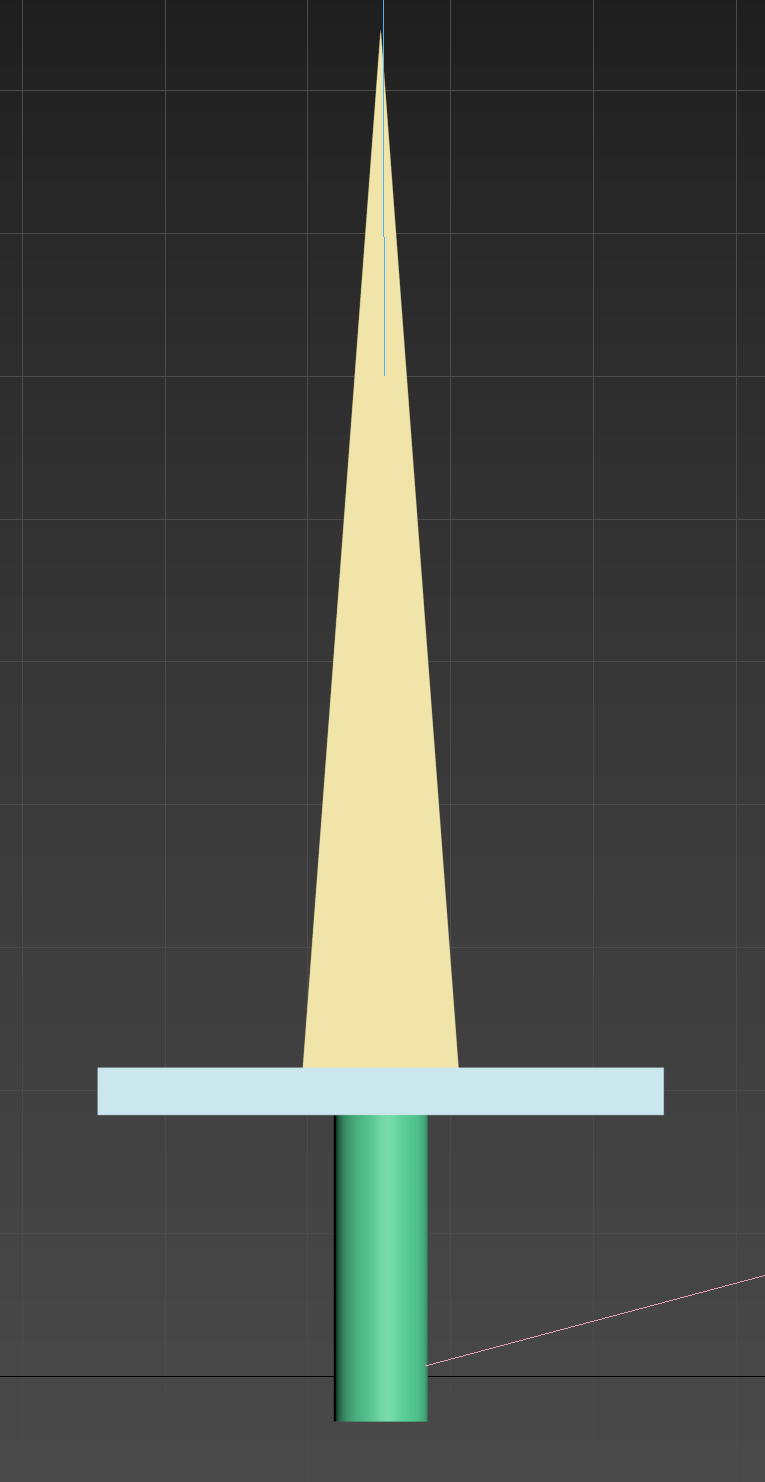
\includegraphics[width=0.2\textwidth]{imagenes/espada.png}
    \caption{Forma final de la espada.}
\end{figure}
\end{itemize}

\bigskip

Voy a dividir la configuración de las manos y de la espada en distintas subsecciones.

\subsection{Configuración de las manos}

Para la animación del cambio de mano, he utilizado los siguientes \textit{keyframes} para la mano más a la izquierda de la escena:

\begin{itemize}
    \item \textbf{Instante 0: }La mano se encuentra en su posición inicial, alejada de la otra mano.
    \item \textbf{Instante 20: }La mano se ha acercado a la otra para darle la espada.
\end{itemize}

Las curvas de la animación son:

% curvas
\begin{figure}[H]
   \centering
   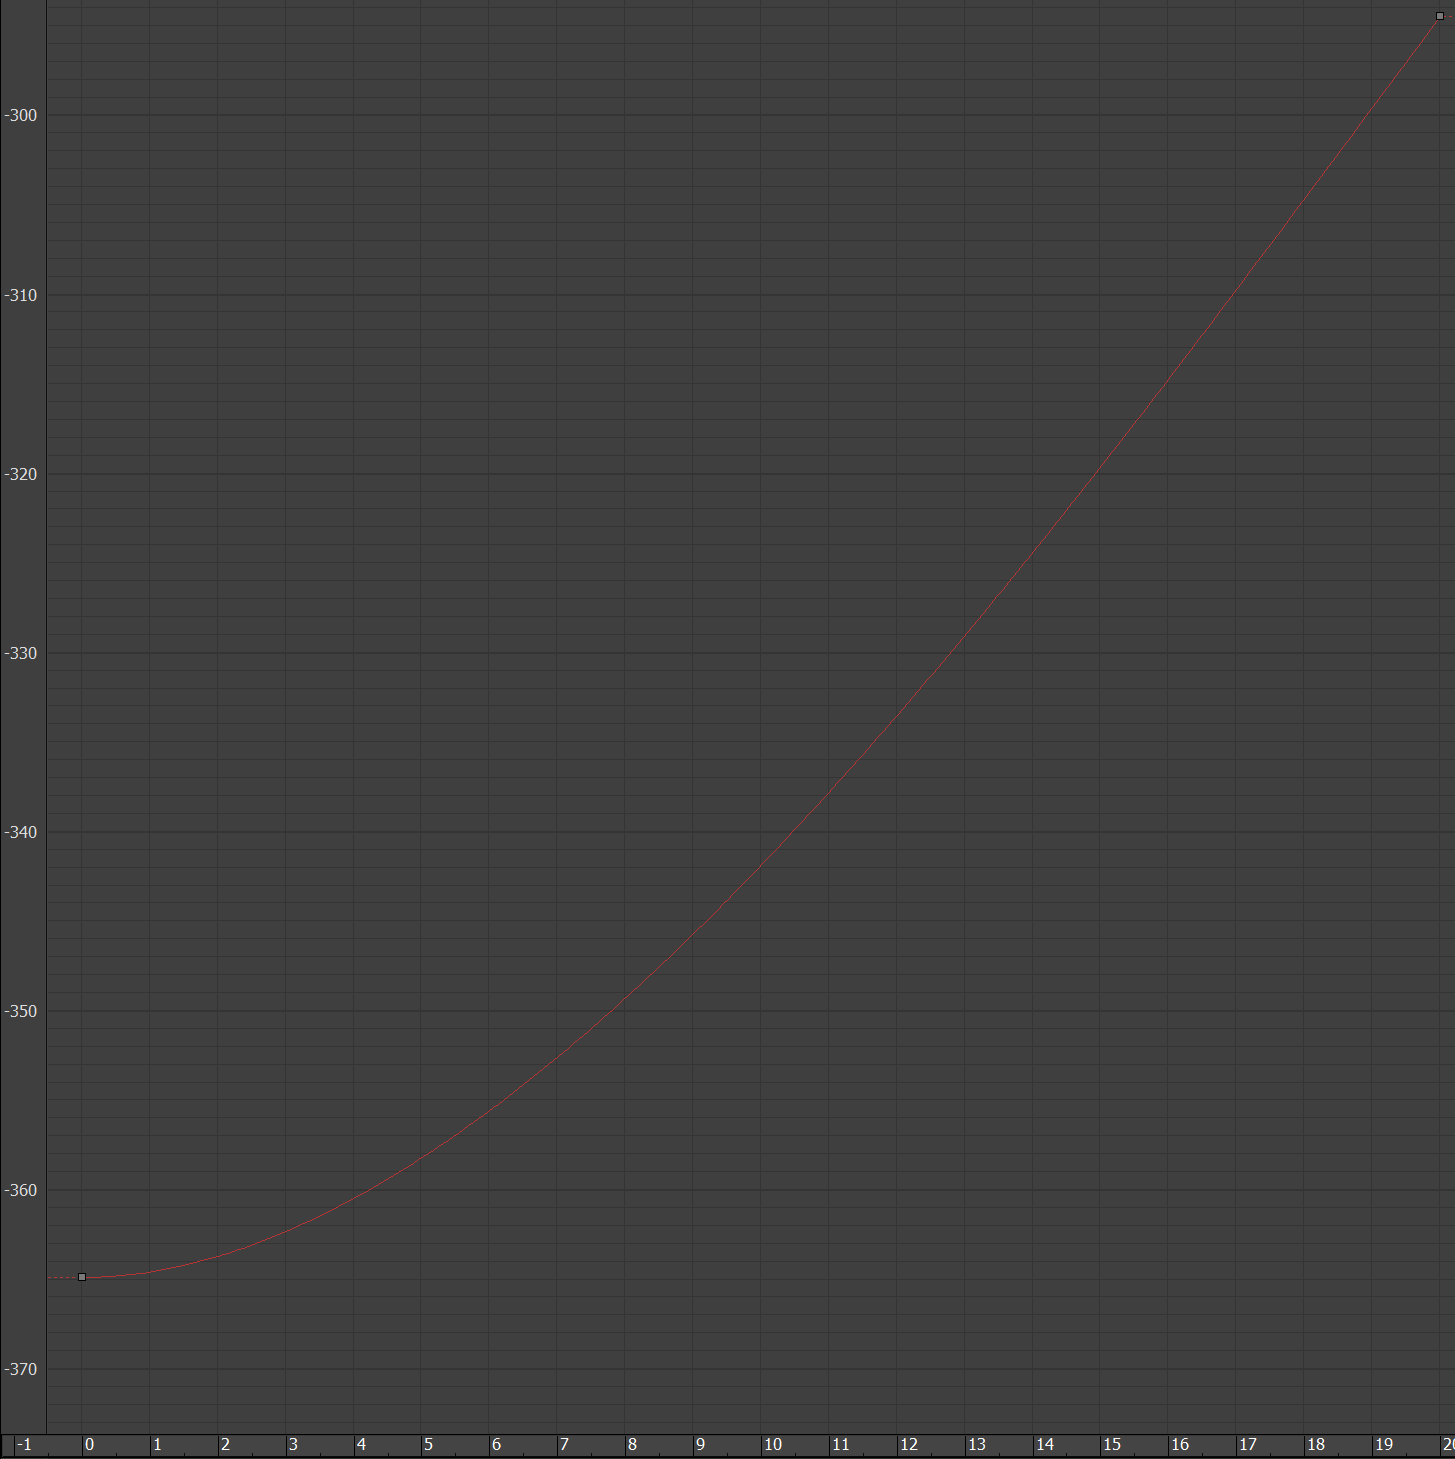
\includegraphics[width=0.6\textwidth]{imagenes/manos/izquierda/posX.png}
   \caption{Curva que representa la posición en el eje X de la mano izquierda.}
\end{figure}


% Como se puede ver, en todas las curvas he usado la forma por defecto \textit{Slow-in/Slow-out}, ya que genera unos resultados más orgánicos y acordes a estas extremidades.

Como se puede observar, he usado una curva de aceleración al principio, para simular la aceleración necesaria que requiere la mano y para intentar representar que la mano le ha lanzado la espada a la otra. Gracias a esta curva, se le puede transferir la velocidad a la espada de manera más o menos realista.

\bigskip


Mientras que la animación para la mano más a la derecha de la escena es: 

\begin{itemize}
    \item \textbf{Instante 30: }La mano se encuentra en su posición inicial y ha recibido la espada de la otra mano.
    \item \textbf{Instante 65: }Ahora la mano se ha dirigido a la plataforma de abajo de la grúa para dejar la espada.
    \item \textbf{Instante 70: }La mano se encuentra en la misma posición, encima de la plataforma. Esto lo he hecho así para simular la espera asociada a abrir la mano para dejar la espada.
    \item \textbf{Instante 90: }Finalmente la mano vuelve a la posición inicial.
\end{itemize}

Las curvas de animación para esta mano son:

\begin{figure}[H]
   \centering
   % curvas
   \begin{subfigure}[t]{0.32\textwidth}
       \centering
       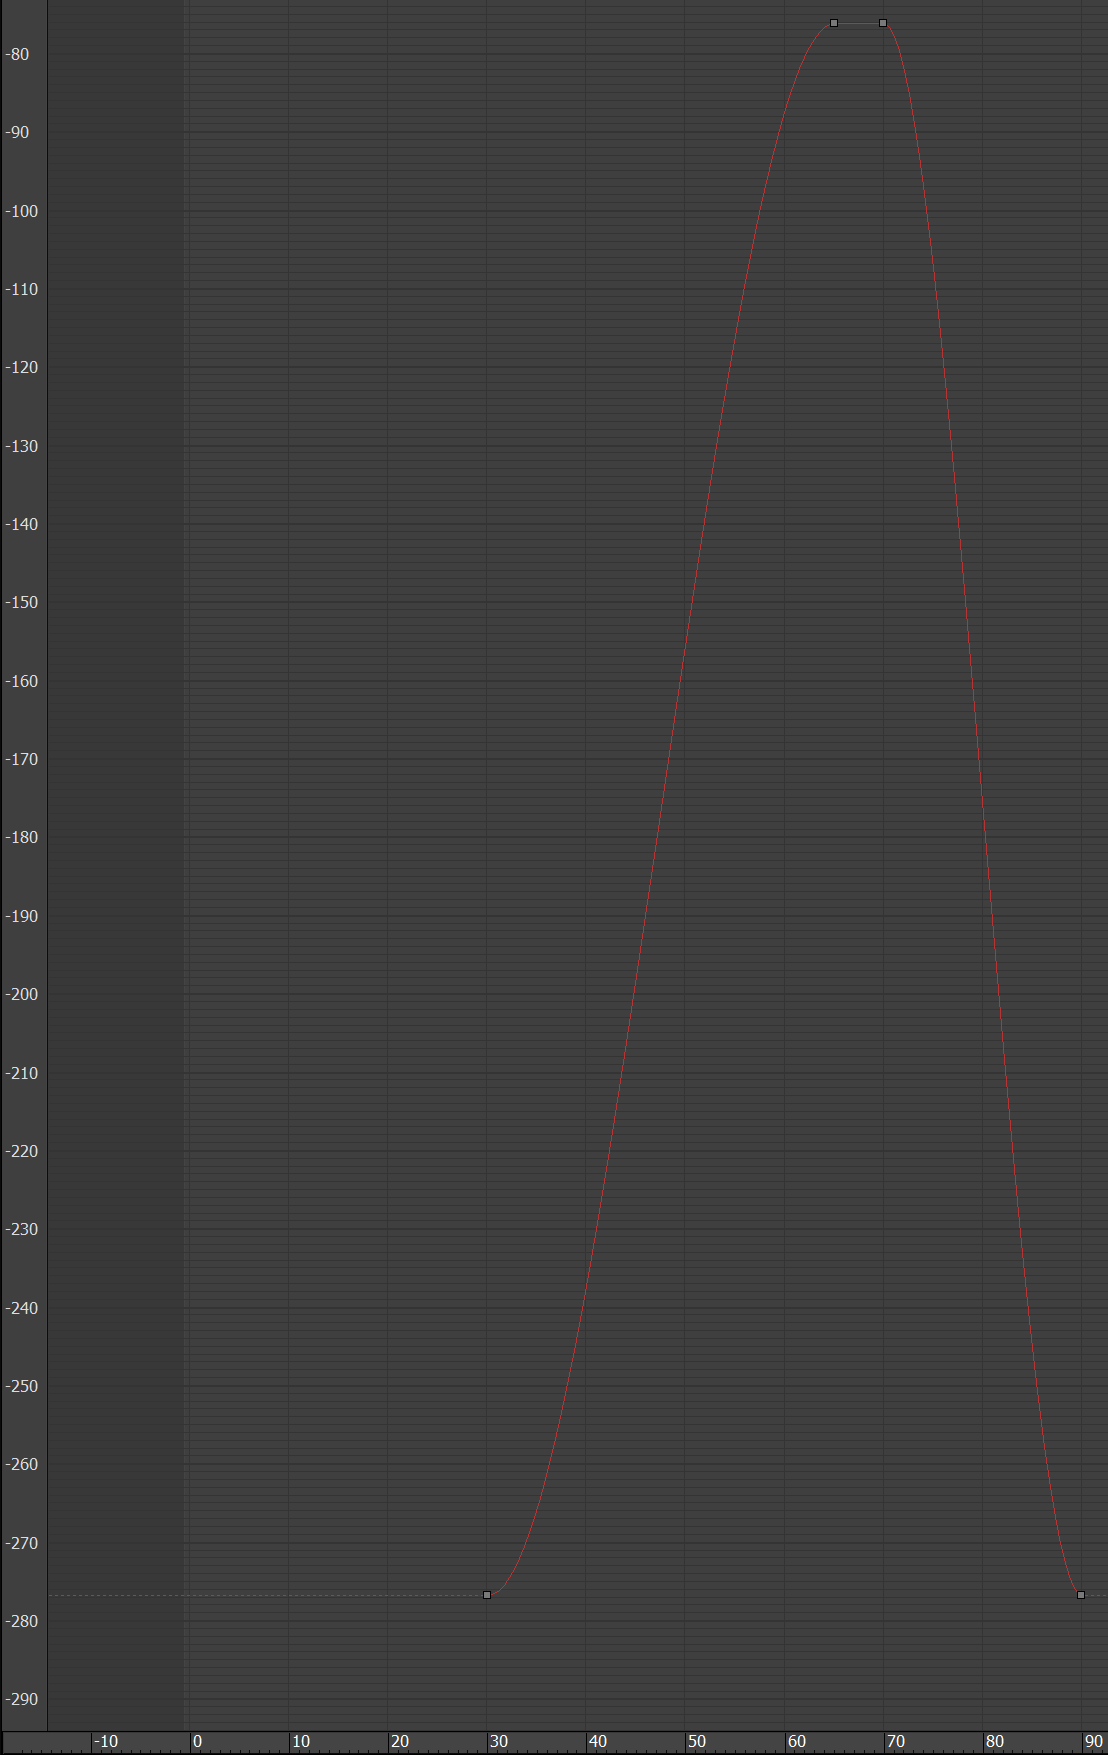
\includegraphics[width=\textwidth]{imagenes/manos/derecha/posX.png}
       \caption{Curva que representa la posición en el eje X de la mano derecha.}
    \end{subfigure}
   \hfill
    \begin{subfigure}[t]{0.32\textwidth}
       \centering
       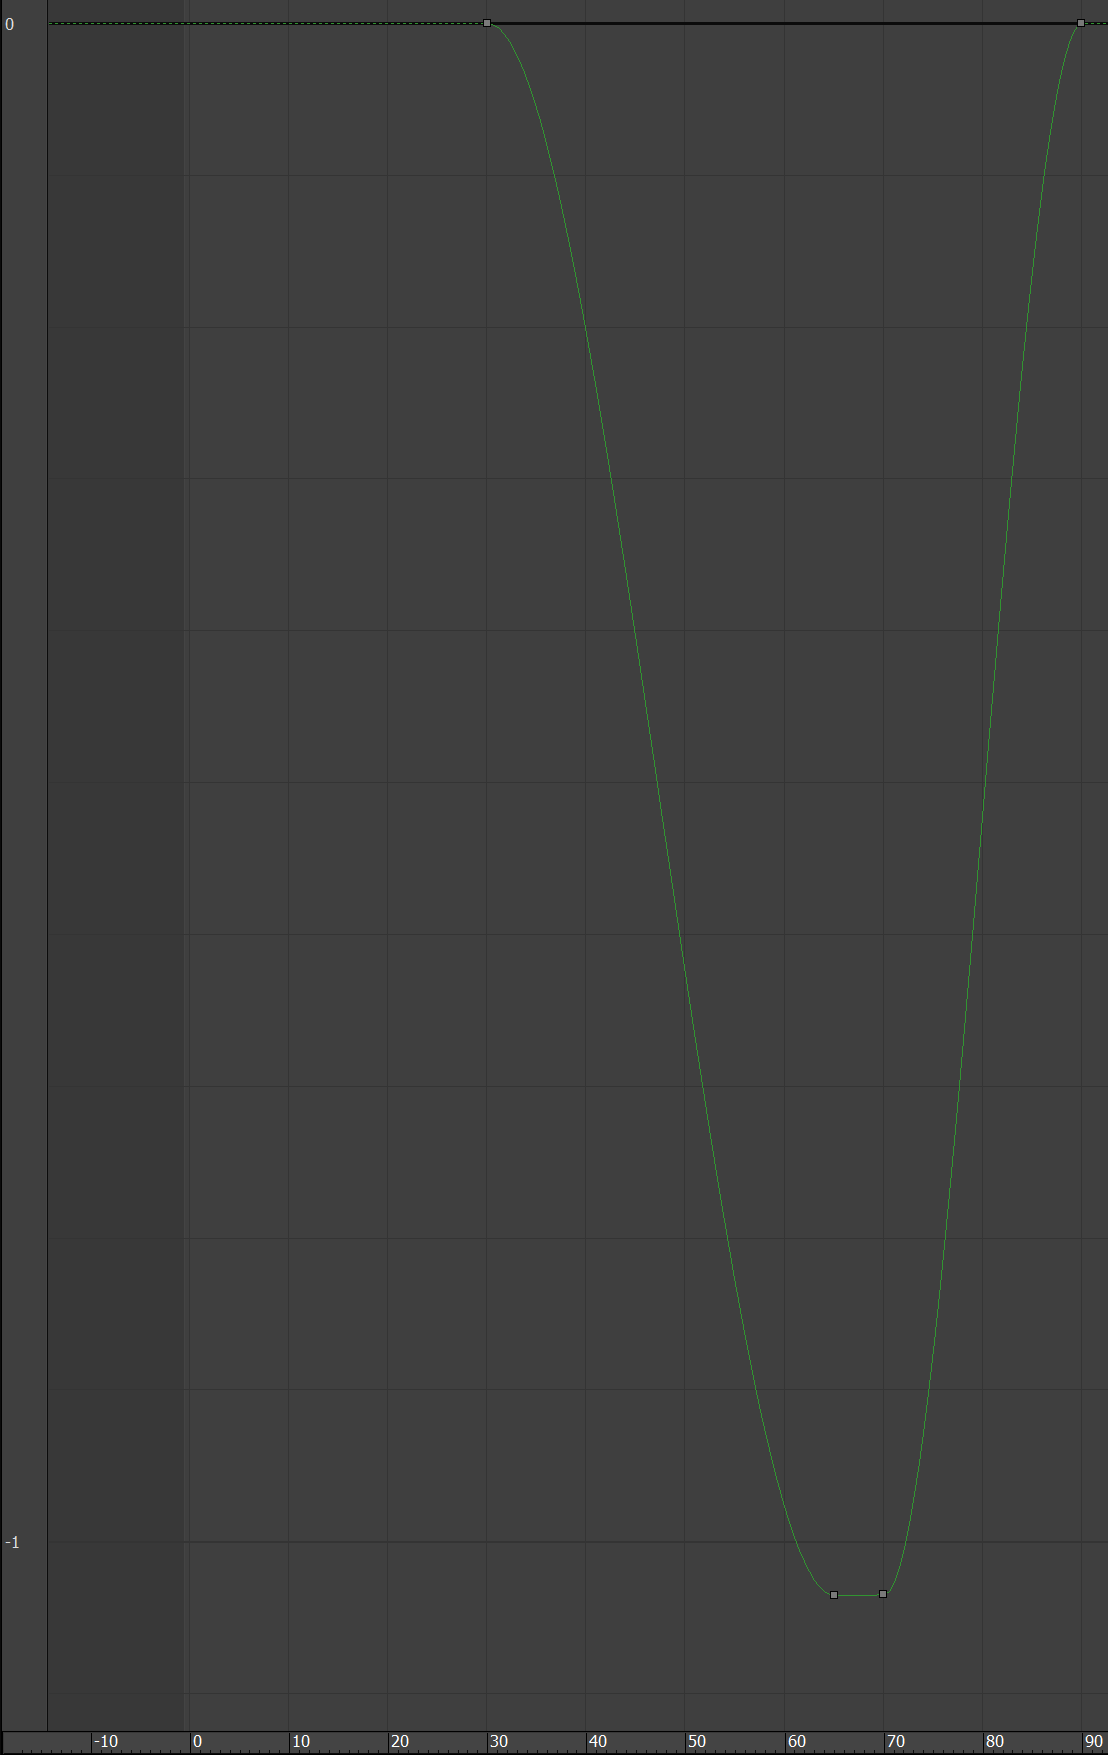
\includegraphics[width=\textwidth]{imagenes/manos/derecha/posY.png}
       \caption{Curva que representa la posición en el eje Y de la mano derecha.}
    \end{subfigure}
   \hfill
    \begin{subfigure}[t]{0.32\textwidth}
       \centering
       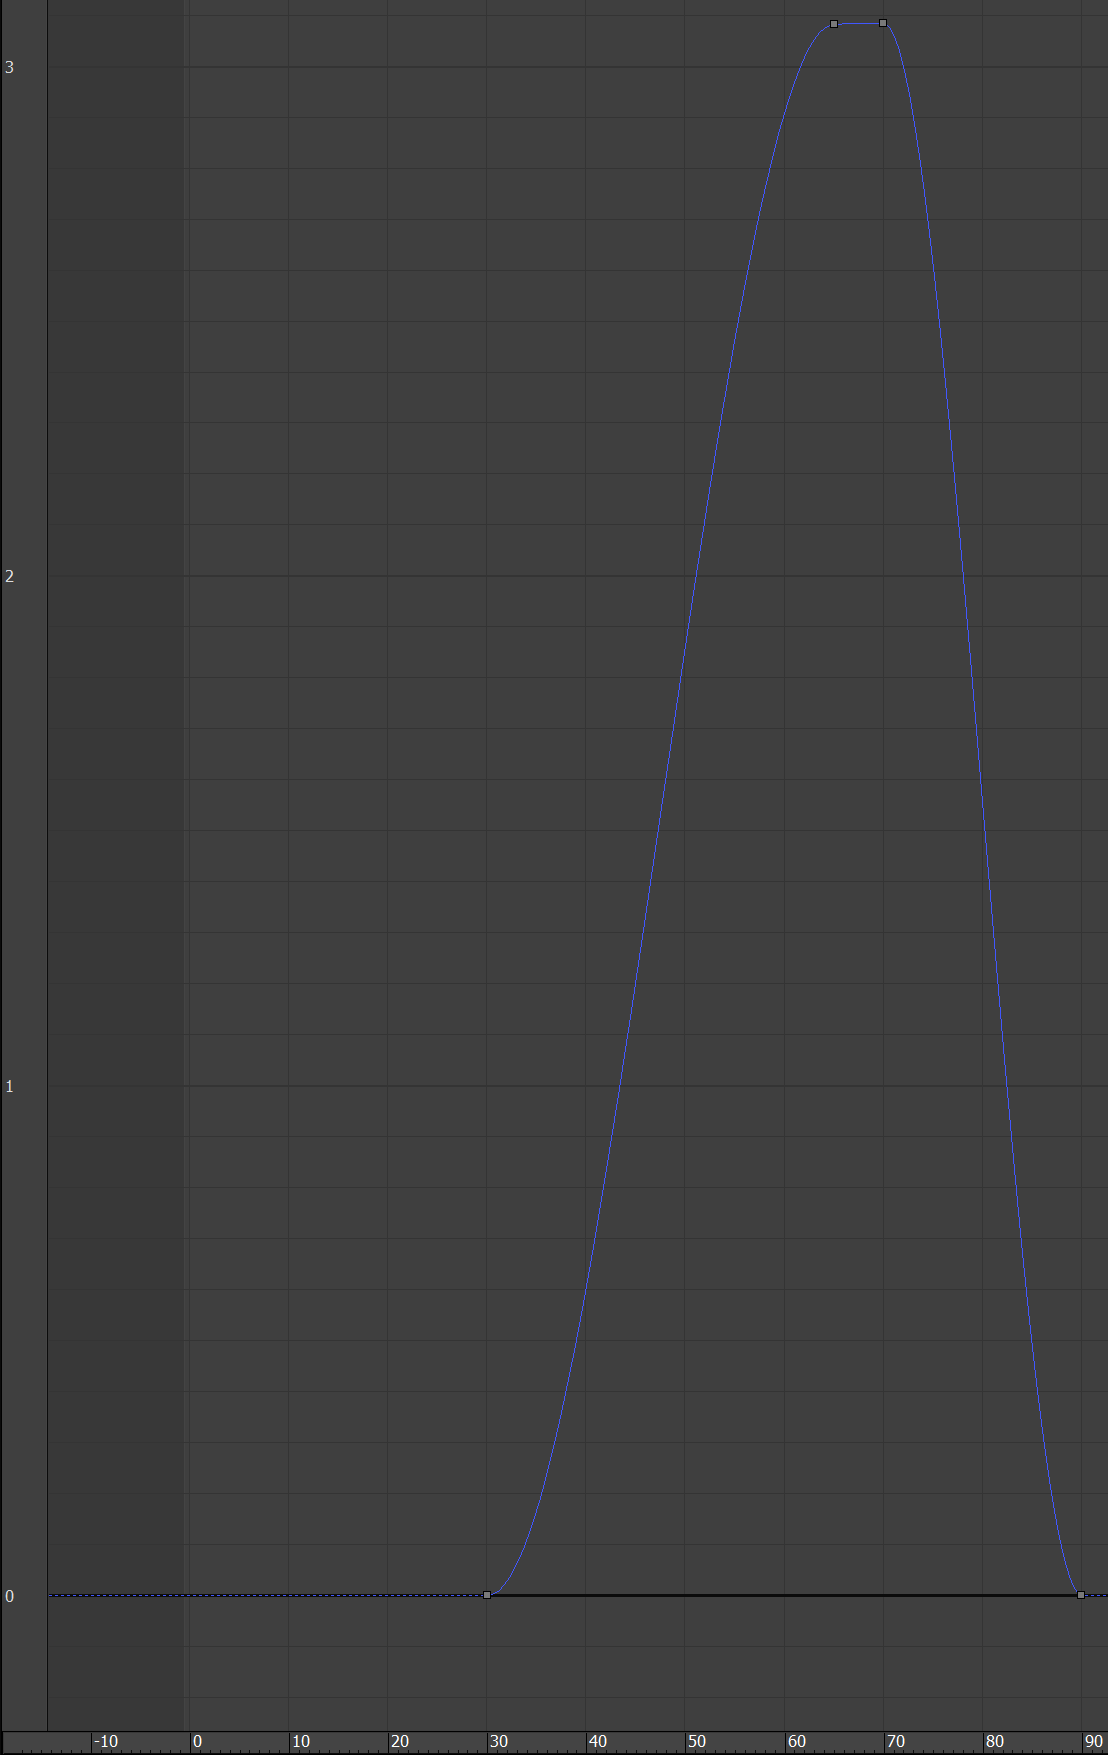
\includegraphics[width=\textwidth]{imagenes/manos/derecha/posZ.png}
       \caption{Curva que representa la posición en el eje Z de la mano derecha.}
    \end{subfigure}
    \caption{Curvas de animación de la mano derecha.}
\end{figure}


% De nuevo, se puede ver que en todas las curvas se ha utilizado la misma forma que para la otra mano, para dar un resultado más realista. 
En esta mano he utilizado la curva por defecto \textit{Slow-in/Slow-out} para todas las curvas, ya que da un resultado convincente, sobre todo cuando debe parar para dejar la espada en la plataforma, que desacelera progresivamente, similar a como se haría en la realidad.

\bigskip

Además, se puede observar como hay una animación en el eje Z. Esto es debido a que la plataforma se encuentra ligeramente más alta que los brazos, haciendo que este tenga que subir un poco y luego bajar para llegar a su posición inicial. Se podría haber bajado la plataforma un poco, para estar a la misma altura ambas, pero me di cuenta demasiado avanzado en el proceso y he preferido hacer este arreglo.

\bigskip

En cuanto a restricciones, ambas manos no tienen restricción de ningún tipo, es la espada la que tiene restricciones.


\subsection{Espada}

% HABLAR SOLO DE LA RESTRICCION DE POSICION, LA OTRA VA EN EL COCHE

La espada tiene dos restricciones, pero en esta sección solo voy a hablar de la de posición, que es la que le corresponde. En la sección del coche hablaré sobre la restricción de rotación.

\bigskip

Para animar el seguimiento de la espada en las manos y las plataformas, se debe hacer con un \textit{Position Constraint} o un \textit{Link}. En mi caso he usado el primero, que por defecto solo afecta al canal de la posición.

\bigskip

Después, he elegido como \textit{targets} las manos y la plataforma, animando después el cambio de pesos. El peso inicialmente estará en la mano más a la izquierda de la escena, después estará en la otra mano y finalmente todo el peso se encontrará en un \textit{dummy} que hay en la plataforma.

% foto de los pesos
\begin{figure}[H]
    \centering
    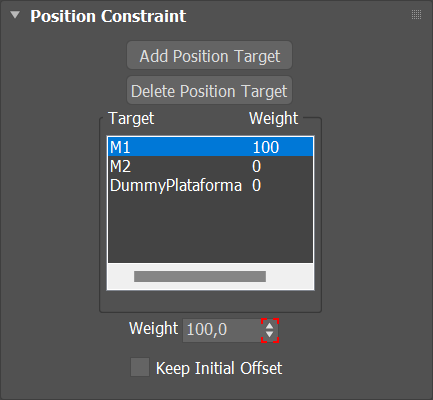
\includegraphics[width=0.4\textwidth]{imagenes/espada/pesosPC.png}
    \caption{Objetivos utilizados para esta restricción.}
 \end{figure}

Los \textit{keyframes} referentes a este \textit{constraint} son:

\begin{itemize}
    \item \textbf{Instante 20: }Todo el peso se encuentra en la mano izquierda inicialmente.
    \item \textbf{Instante 27: }Ahora todo el peso se encuentra en la otra mano.
    \item \textbf{Instante 65: }No hay ningún cambio, el peso sigue encontrándose en la mano derecha.
    \item \textbf{Instante 70: }El peso ahora se encuentra en el \textit{dummy} de la plataforma.
\end{itemize}

\bigskip

En cuanto a la curva de animación referente al \textit{Position Constraint} es la siguiente:

% curva de animacion
\begin{figure}[H]
   \centering
   % curvas
   \begin{subfigure}[t]{0.27\textwidth}
       \centering
       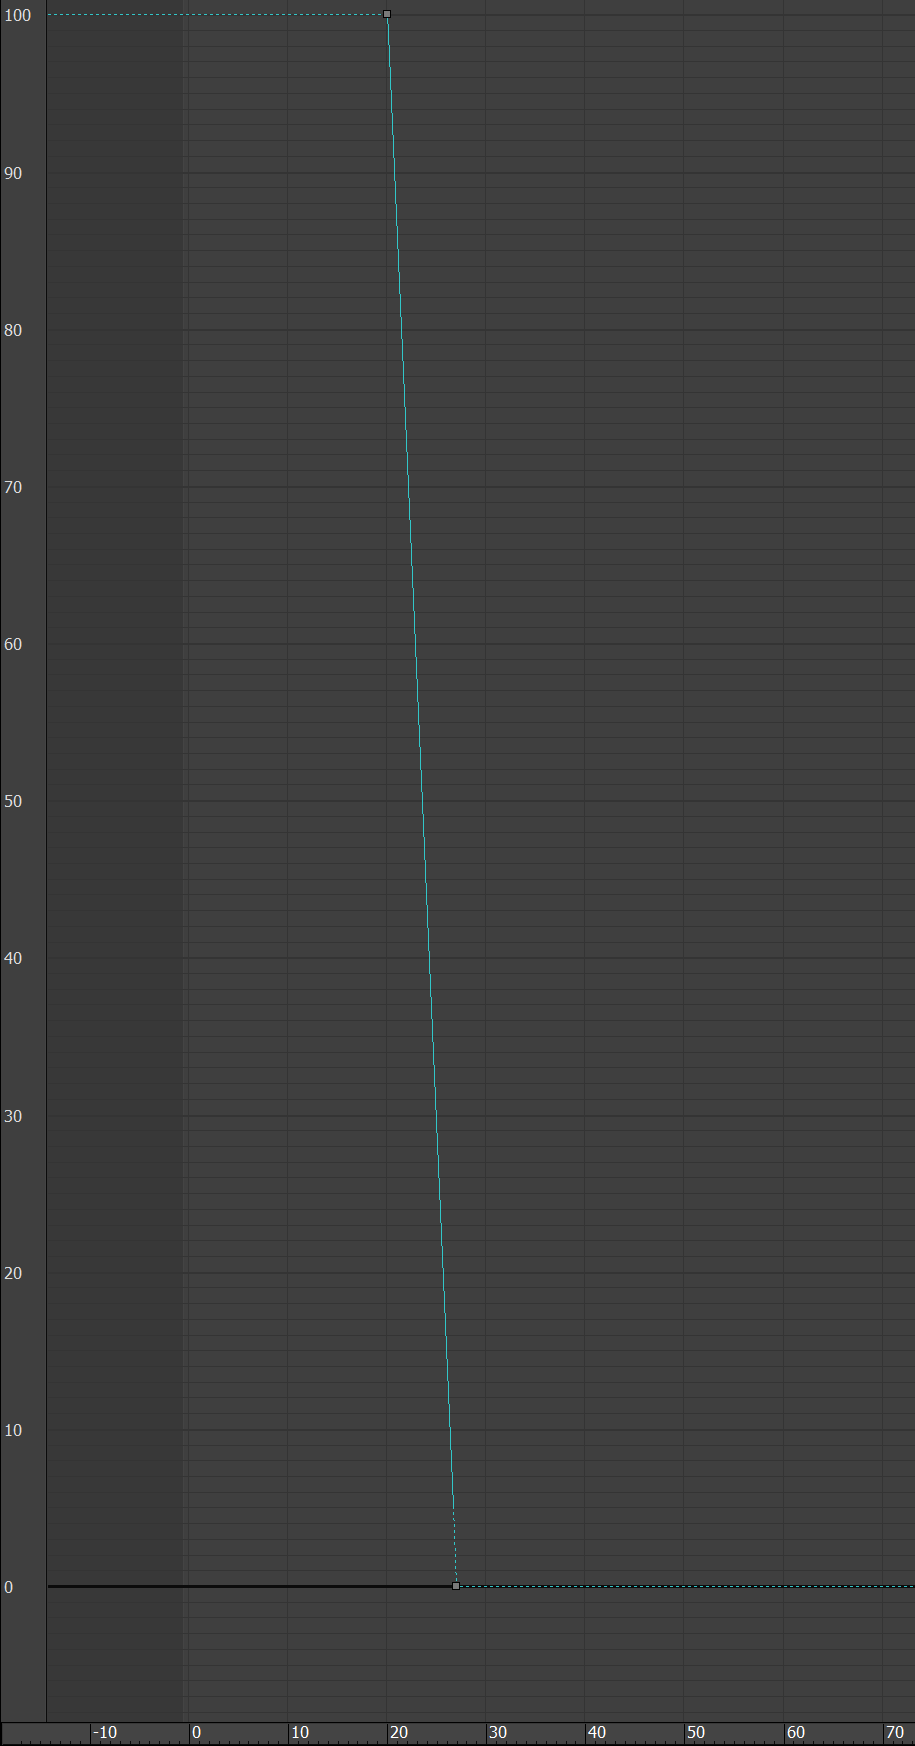
\includegraphics[width=\textwidth]{imagenes/espada/peso0.png}
       \caption{Curva que representa el peso de la mano izquierda con respecto al tiempo.}
    \end{subfigure}
   \hfill
    \begin{subfigure}[t]{0.27\textwidth}
       \centering
       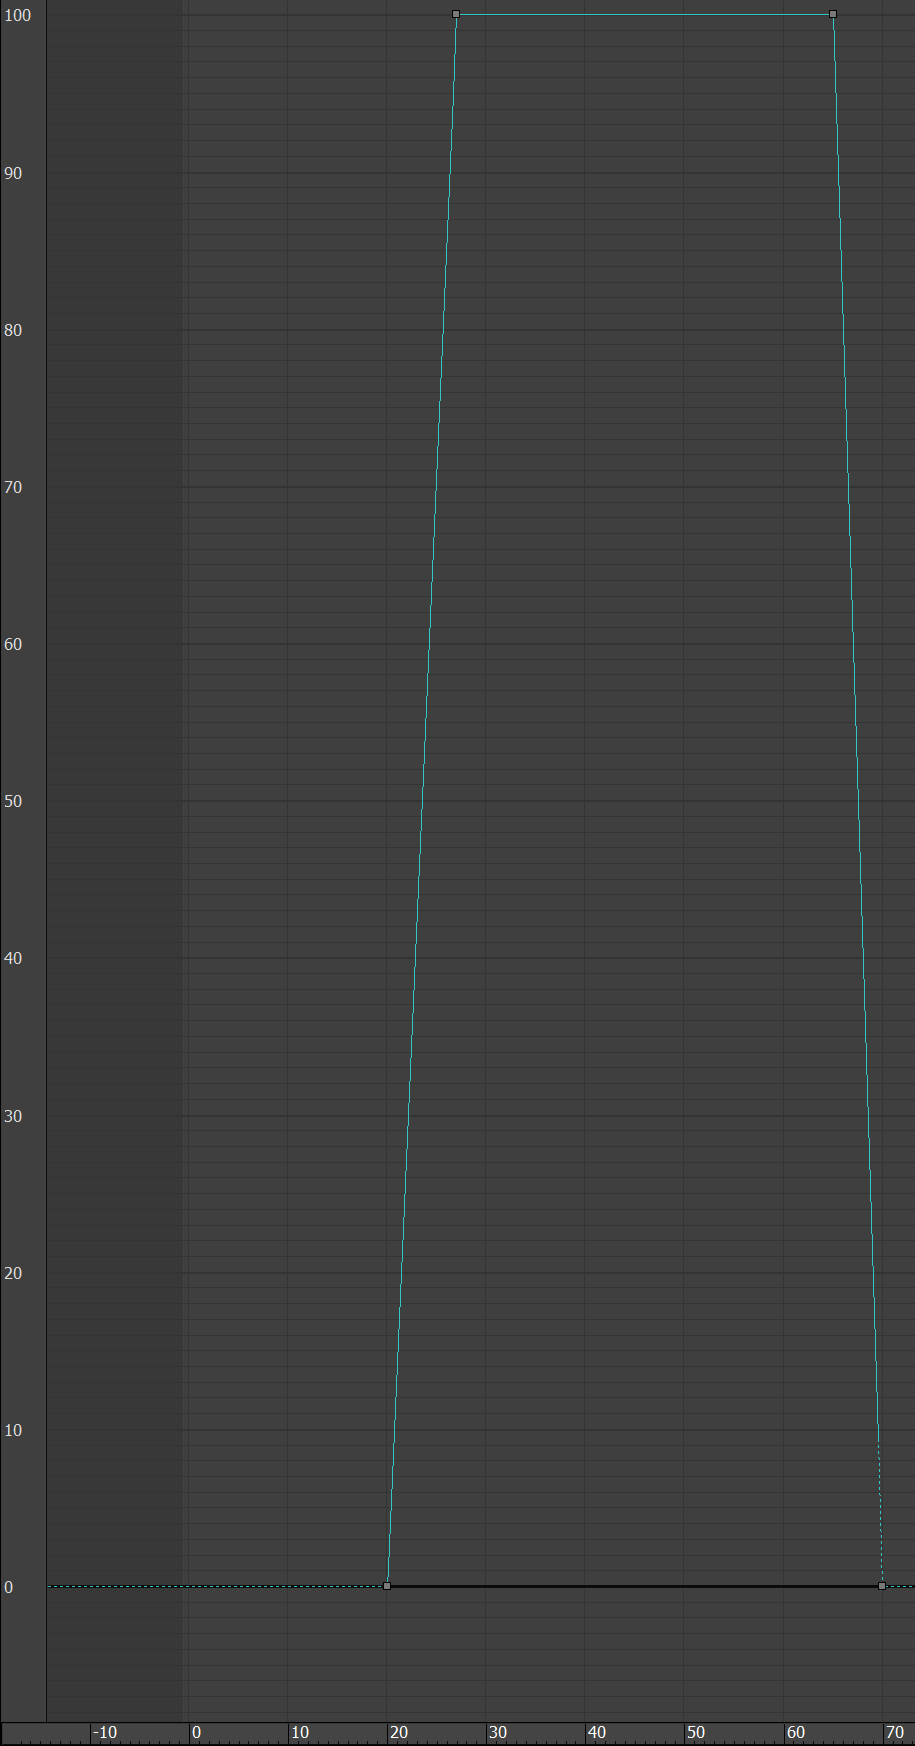
\includegraphics[width=\textwidth]{imagenes/espada/peso1.png}
       \caption{Curva que representa el peso de la mano derecha con respecto al tiempo.}
    \end{subfigure}
   \hfill
    \begin{subfigure}[t]{0.27\textwidth}
       \centering
       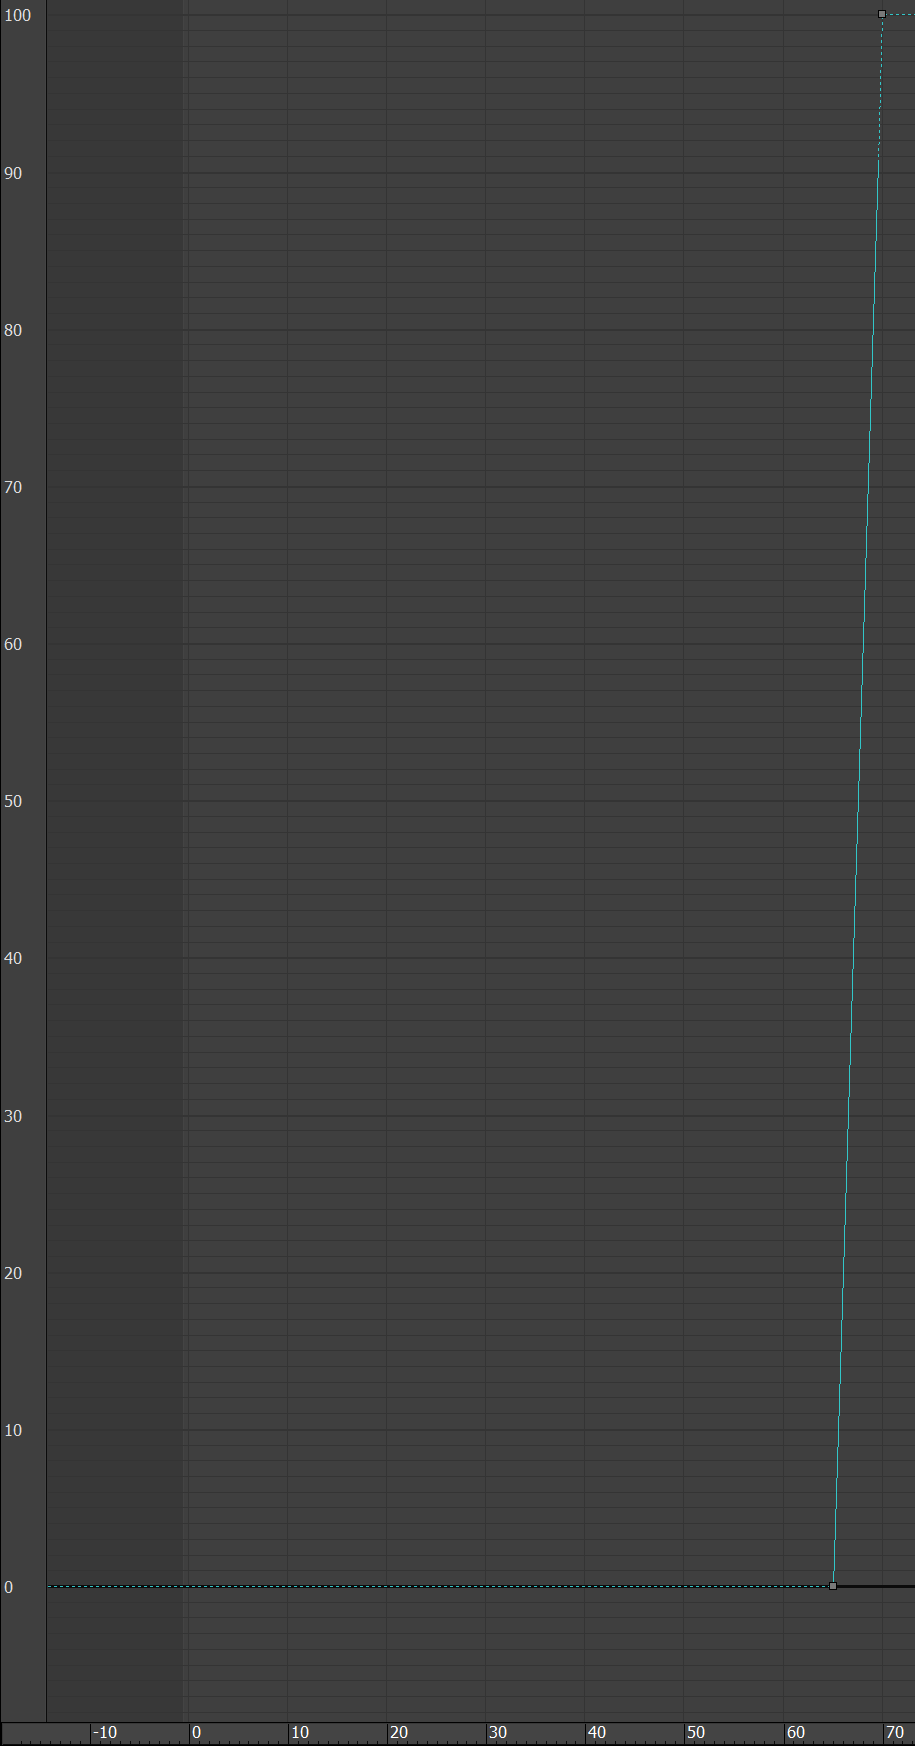
\includegraphics[width=\textwidth]{imagenes/espada/peso2.png}
       \caption{Curva que representa el peso de la plataforma con respecto al tiempo.}
    \end{subfigure}
    \caption{Curvas de los pesos del \textit{Position Constraint}.}
\end{figure}

Como se puede observar, las curvas de animación son lineales. Lo he hecho así para simular el lanzamiento de la espada de la mano izquierda, que le transfiere su velocidad. El paso de la mano derecha a la plataforma lo he hecho de forma lineal también, ya que la mano se posa sobre el siguiente punto en el que debe estar la espada, haciendo que esta no se mueva y no se aprecie diferencia entre distintos tipos de curva.

\bigskip

La configuración del \textit{Position Constraint} es:

\begin{figure}[H]
   \centering
   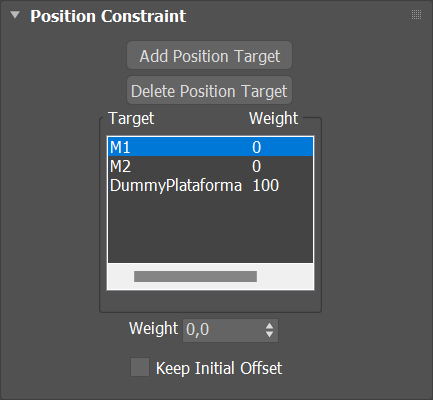
\includegraphics[width=0.4\textwidth]{imagenes/espada/PCconfig.png}
   \caption{Configuración final del \textit{Position Constraint}.}
\end{figure}

\subsection{Resultado final en el cambio de manos}

El resultado final de todo esto es el siguiente:

% fotos de los fotogramas mas importantes.
\begin{figure}[H]
   \centering
\begin{subfigure}[t]{0.48\textwidth}
    \centering
    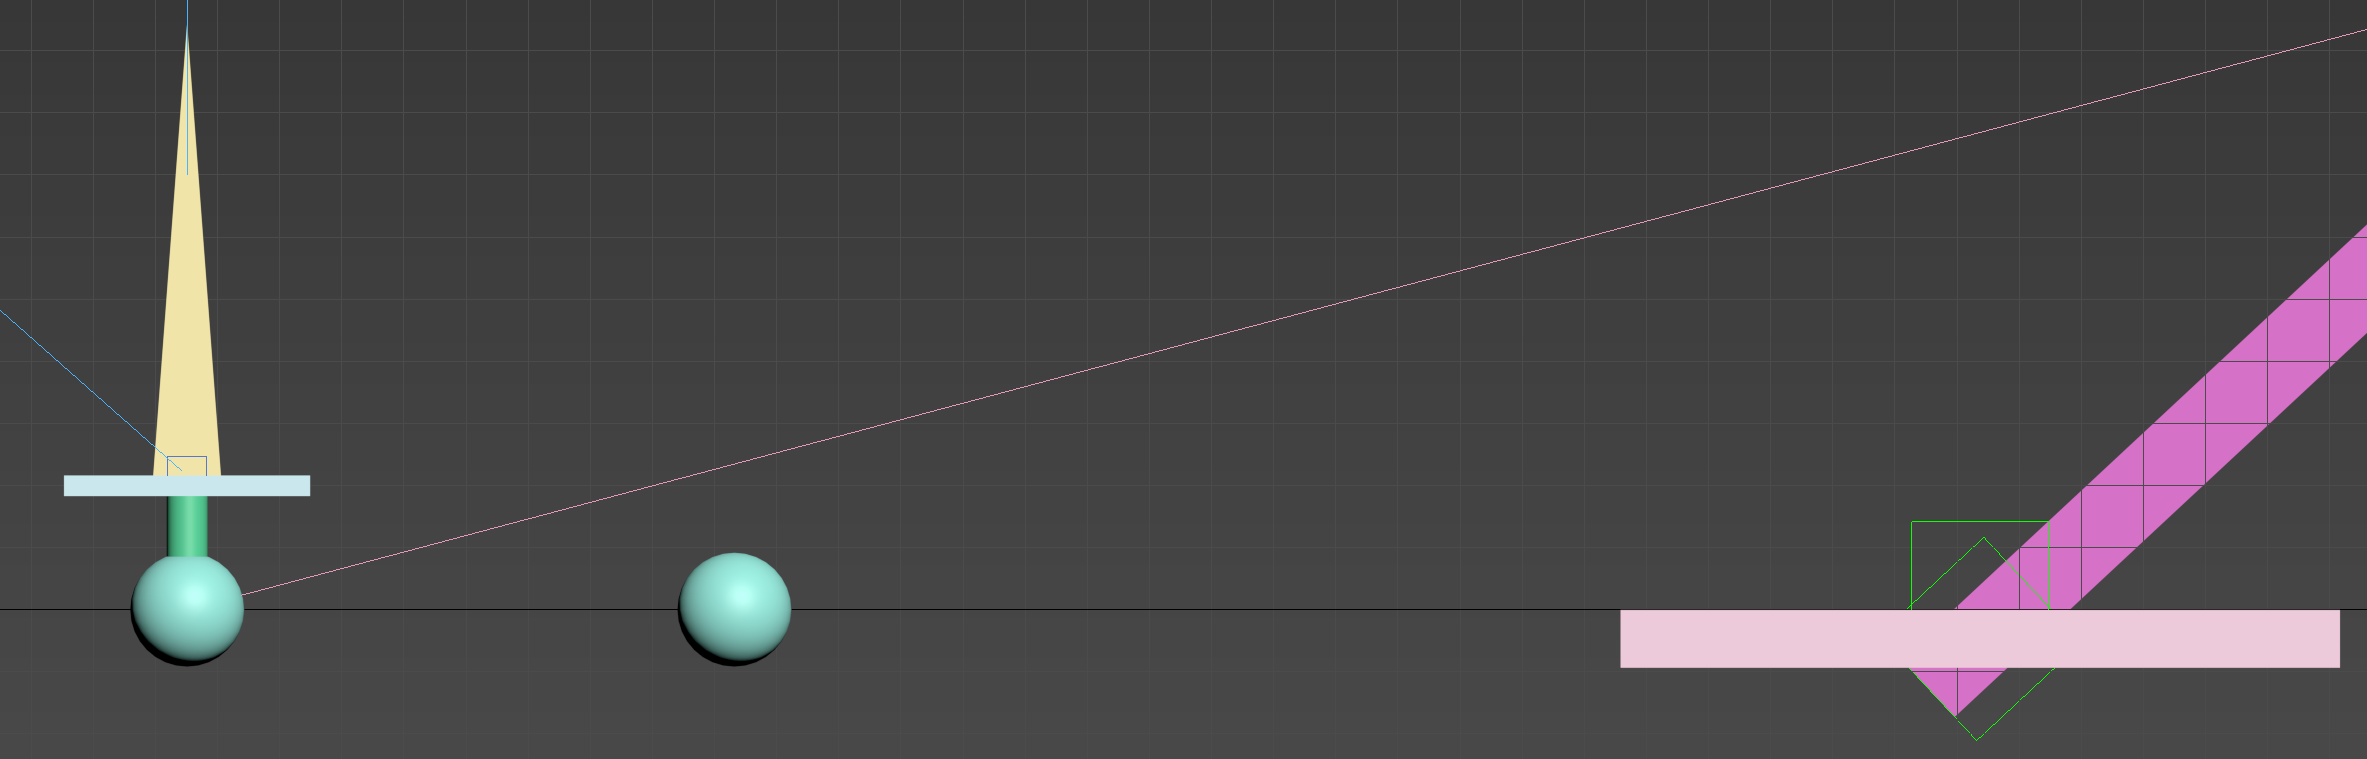
\includegraphics[width=\textwidth]{imagenes/espada/keyframes/0.png}
    \caption{Manos en el instante 0.}
 \end{subfigure}
\hfill
 \begin{subfigure}[t]{0.48\textwidth}
    \centering
    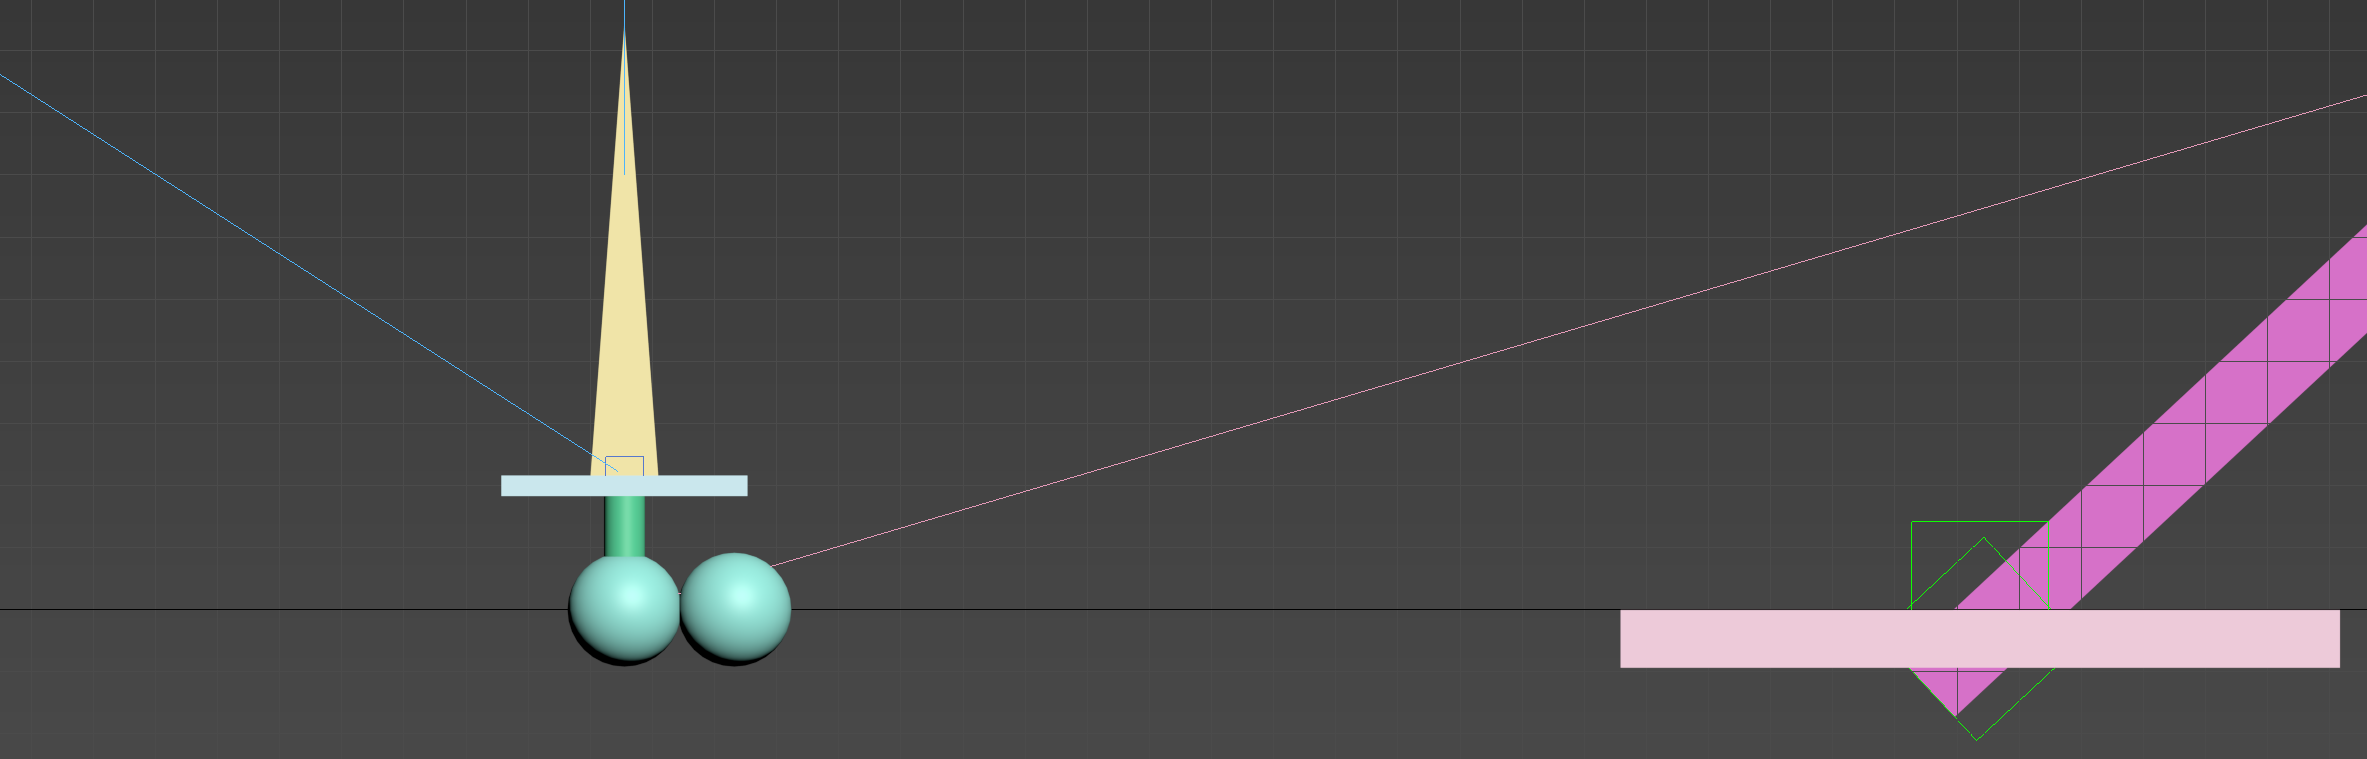
\includegraphics[width=\textwidth]{imagenes/espada/keyframes/20.png}
    \caption{Manos en el instante 20.}
 \end{subfigure}
\hfill
 \begin{subfigure}[t]{0.48\textwidth}
    \centering
    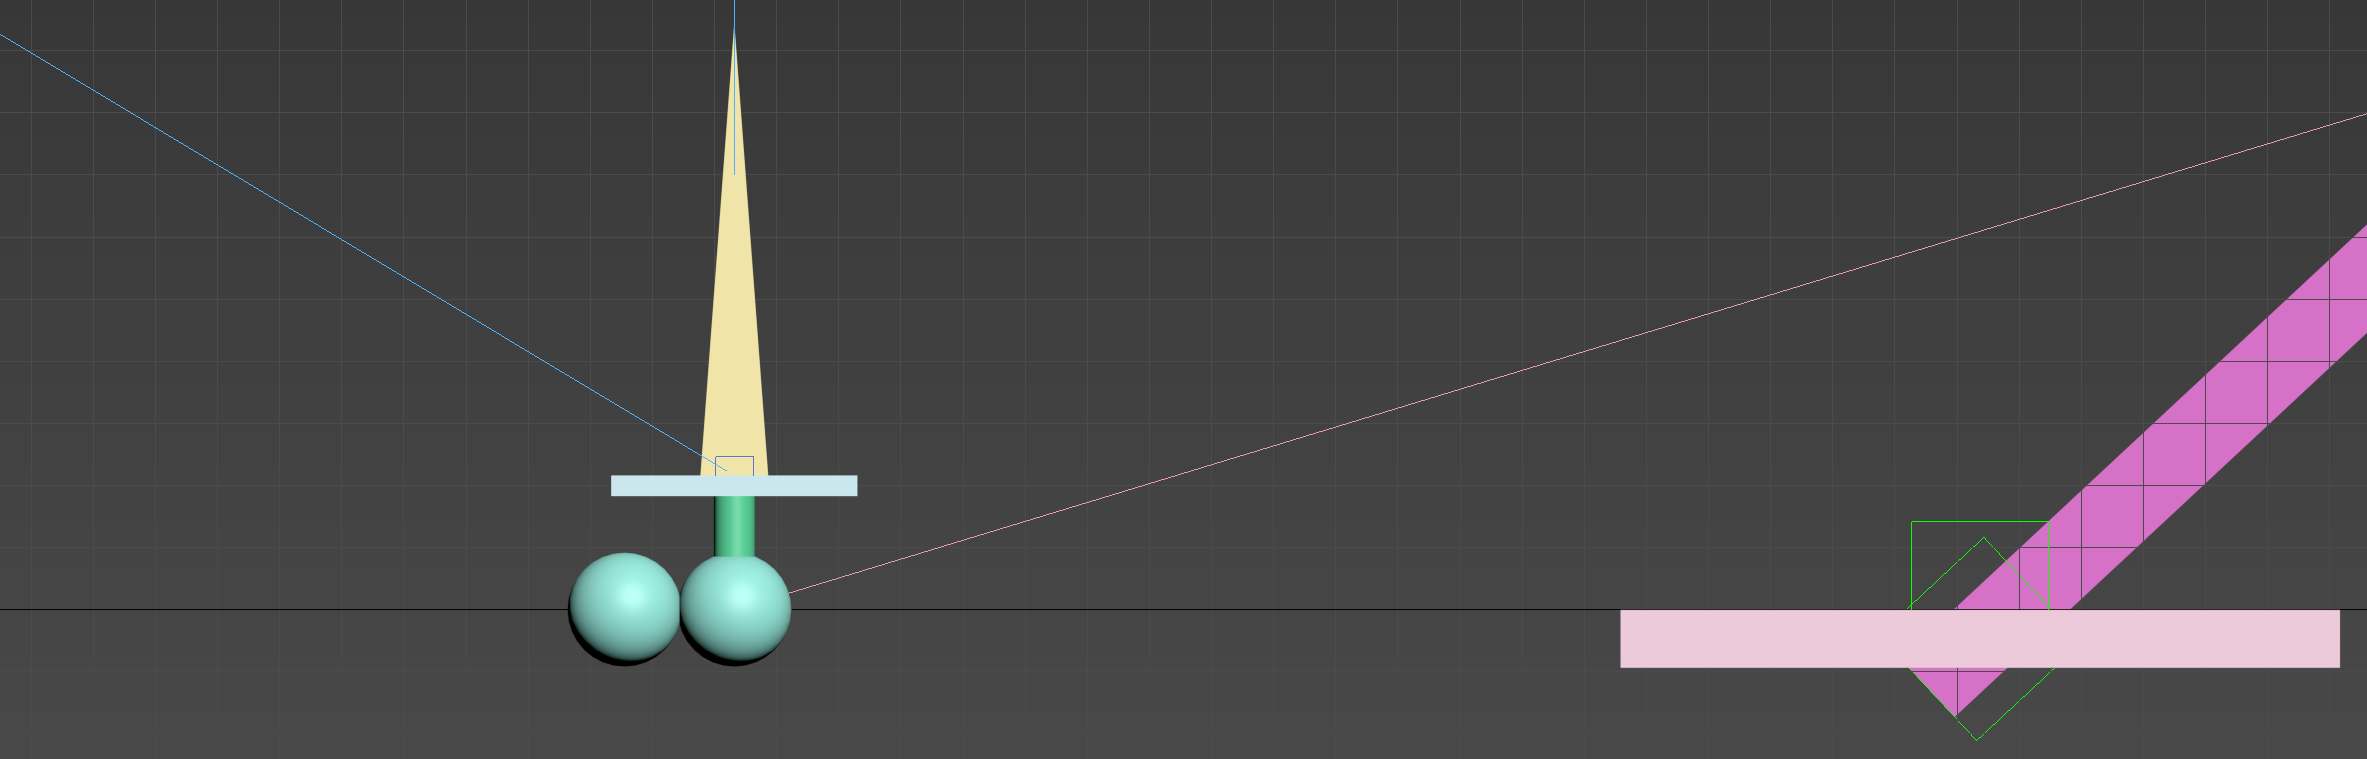
\includegraphics[width=\textwidth]{imagenes/espada/keyframes/27y30.png}
    \caption{Manos en los instantes 27 y 30.}
 \end{subfigure}
\hfill
 \begin{subfigure}[t]{0.48\textwidth}
    \centering
    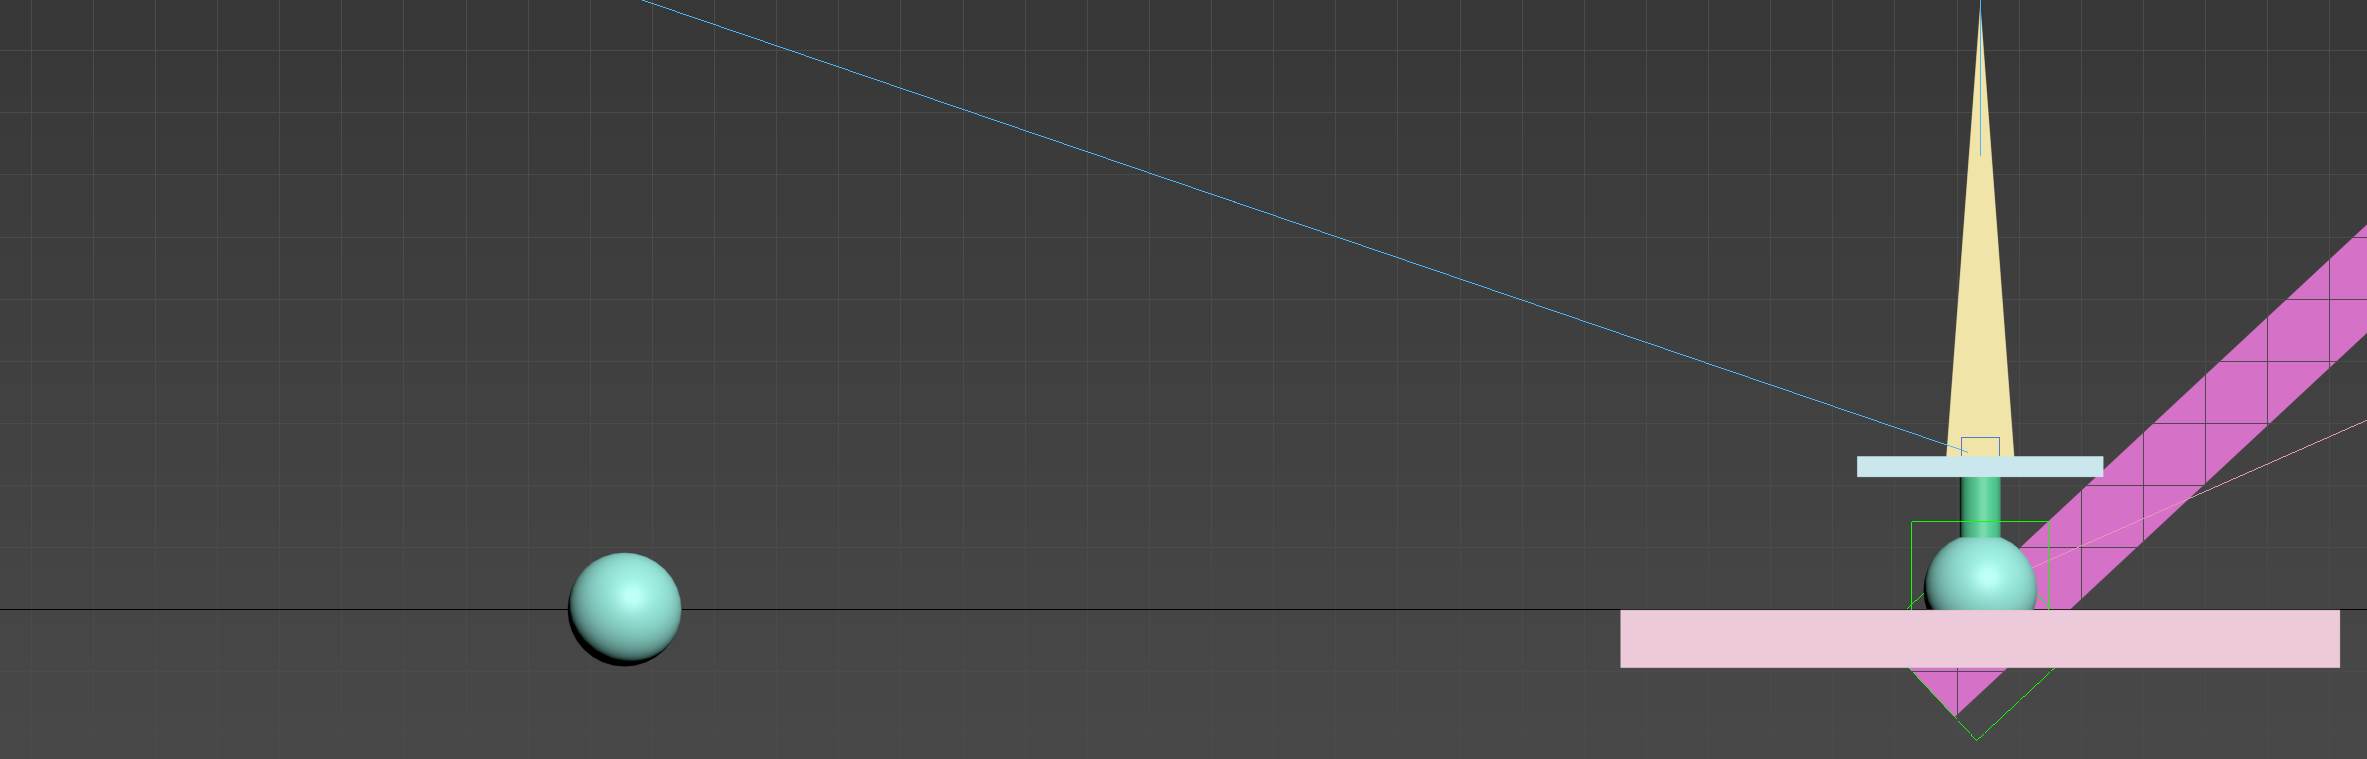
\includegraphics[width=\textwidth]{imagenes/espada/keyframes/65y70.png}
    \caption{Manos en los instantes 65 y 70.}
 \end{subfigure}
\hfill
 \begin{subfigure}[t]{0.48\textwidth}
    \centering
    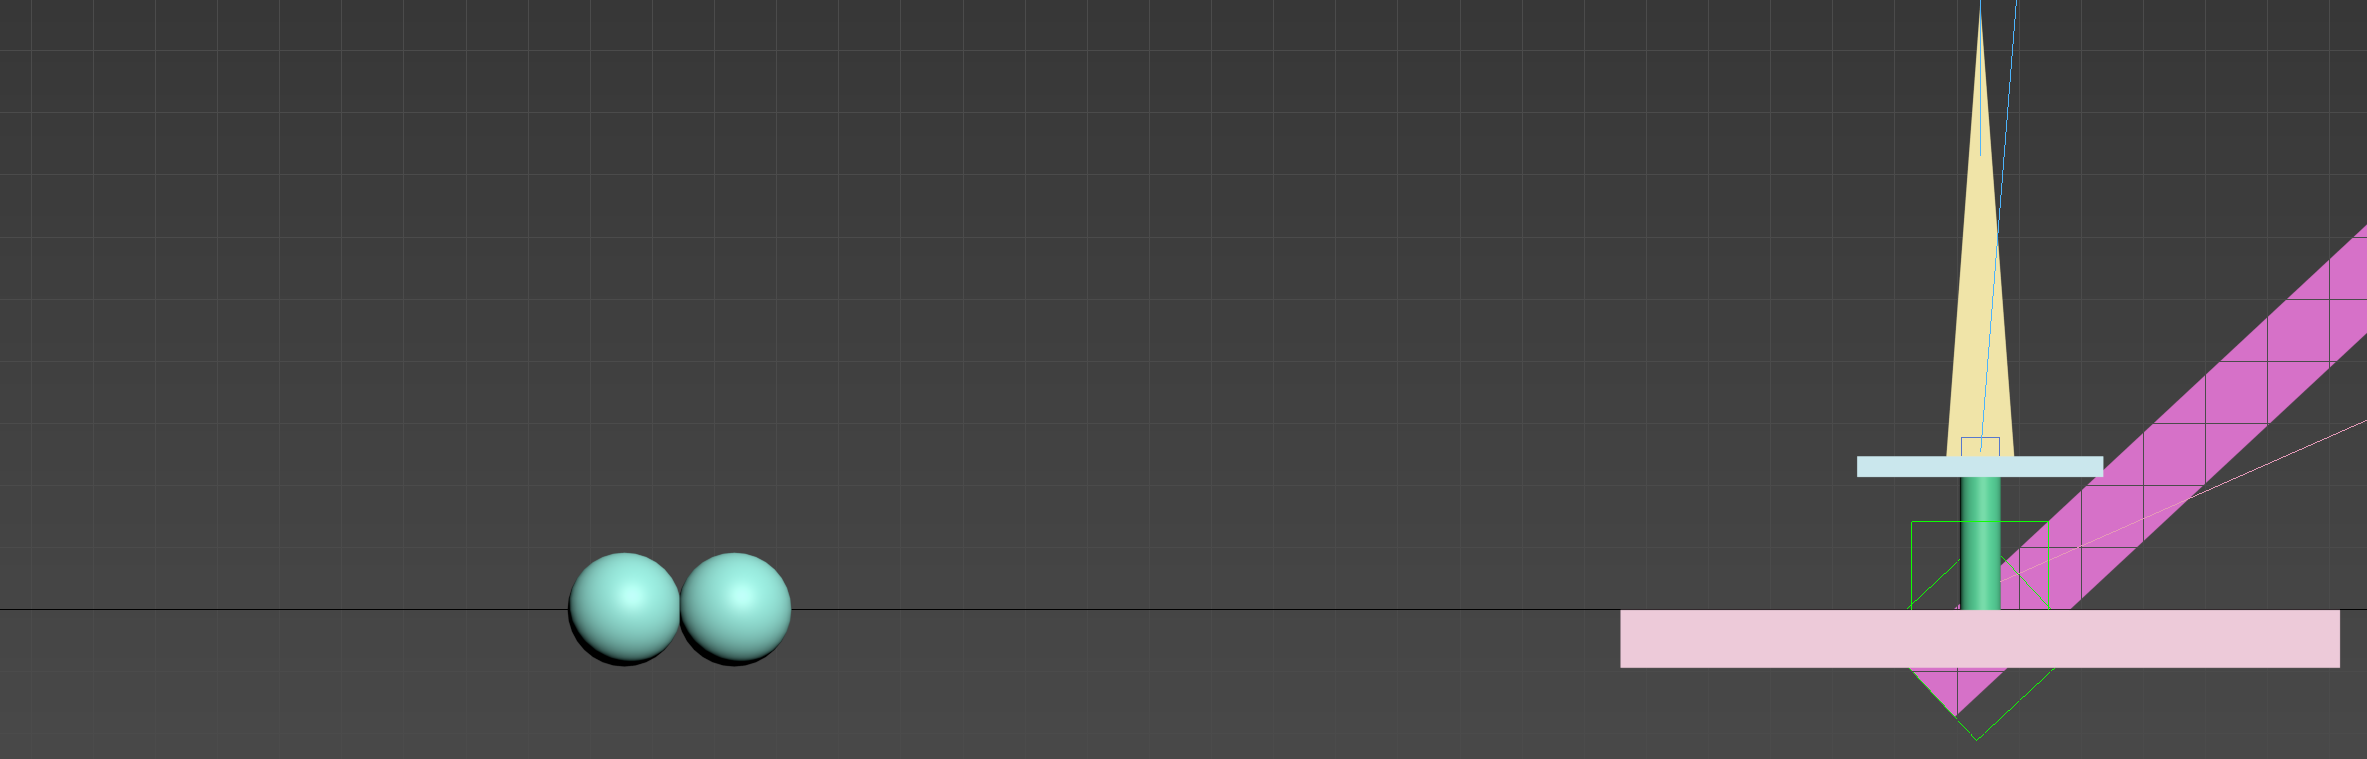
\includegraphics[width=\textwidth]{imagenes/espada/keyframes/90.png}
    \caption{Manos en el instante 90.}
 \end{subfigure}
 \caption{\textit{Keyframes} más importantes de la animación de las manos.}
\end{figure}
\newpage

\section{Grúa}

La composición de la grúa la he realizado usando un cubo achatado, para la unión de ambas plataformas, y dos cubos también achatados para las propias plataformas.

\bigskip

% rescribir
Además, he puesto dos \textit{dummies} en el cubo que une ambas plataformas; es decir, en los extremos del brazo, con el objetivo de que funcione bien la restricción que explicaré a continuación. En cuanto a las plataformas, he movido sus pivotes para que se encuentren pegados a una de las caras, para que al usar la restricción no se solape con el brazo.

\bigskip

En cuanto a las restricciones, he usado un \textit{Position Constraint} en cada plataforma, con su \textit{Target} siendo su \textit{Dummy} respectivo. Esto hace que el brazo pueda girar junto a las plataformas, pero estas últimas siempre paralelas al suelo.

\bigskip

Cabe destacar que estas restricciones no tienen animaciones, al no tener otro objeto al que unirse.

% foto de los dummies, el pivote y general
\begin{figure}[H]
    \centering
    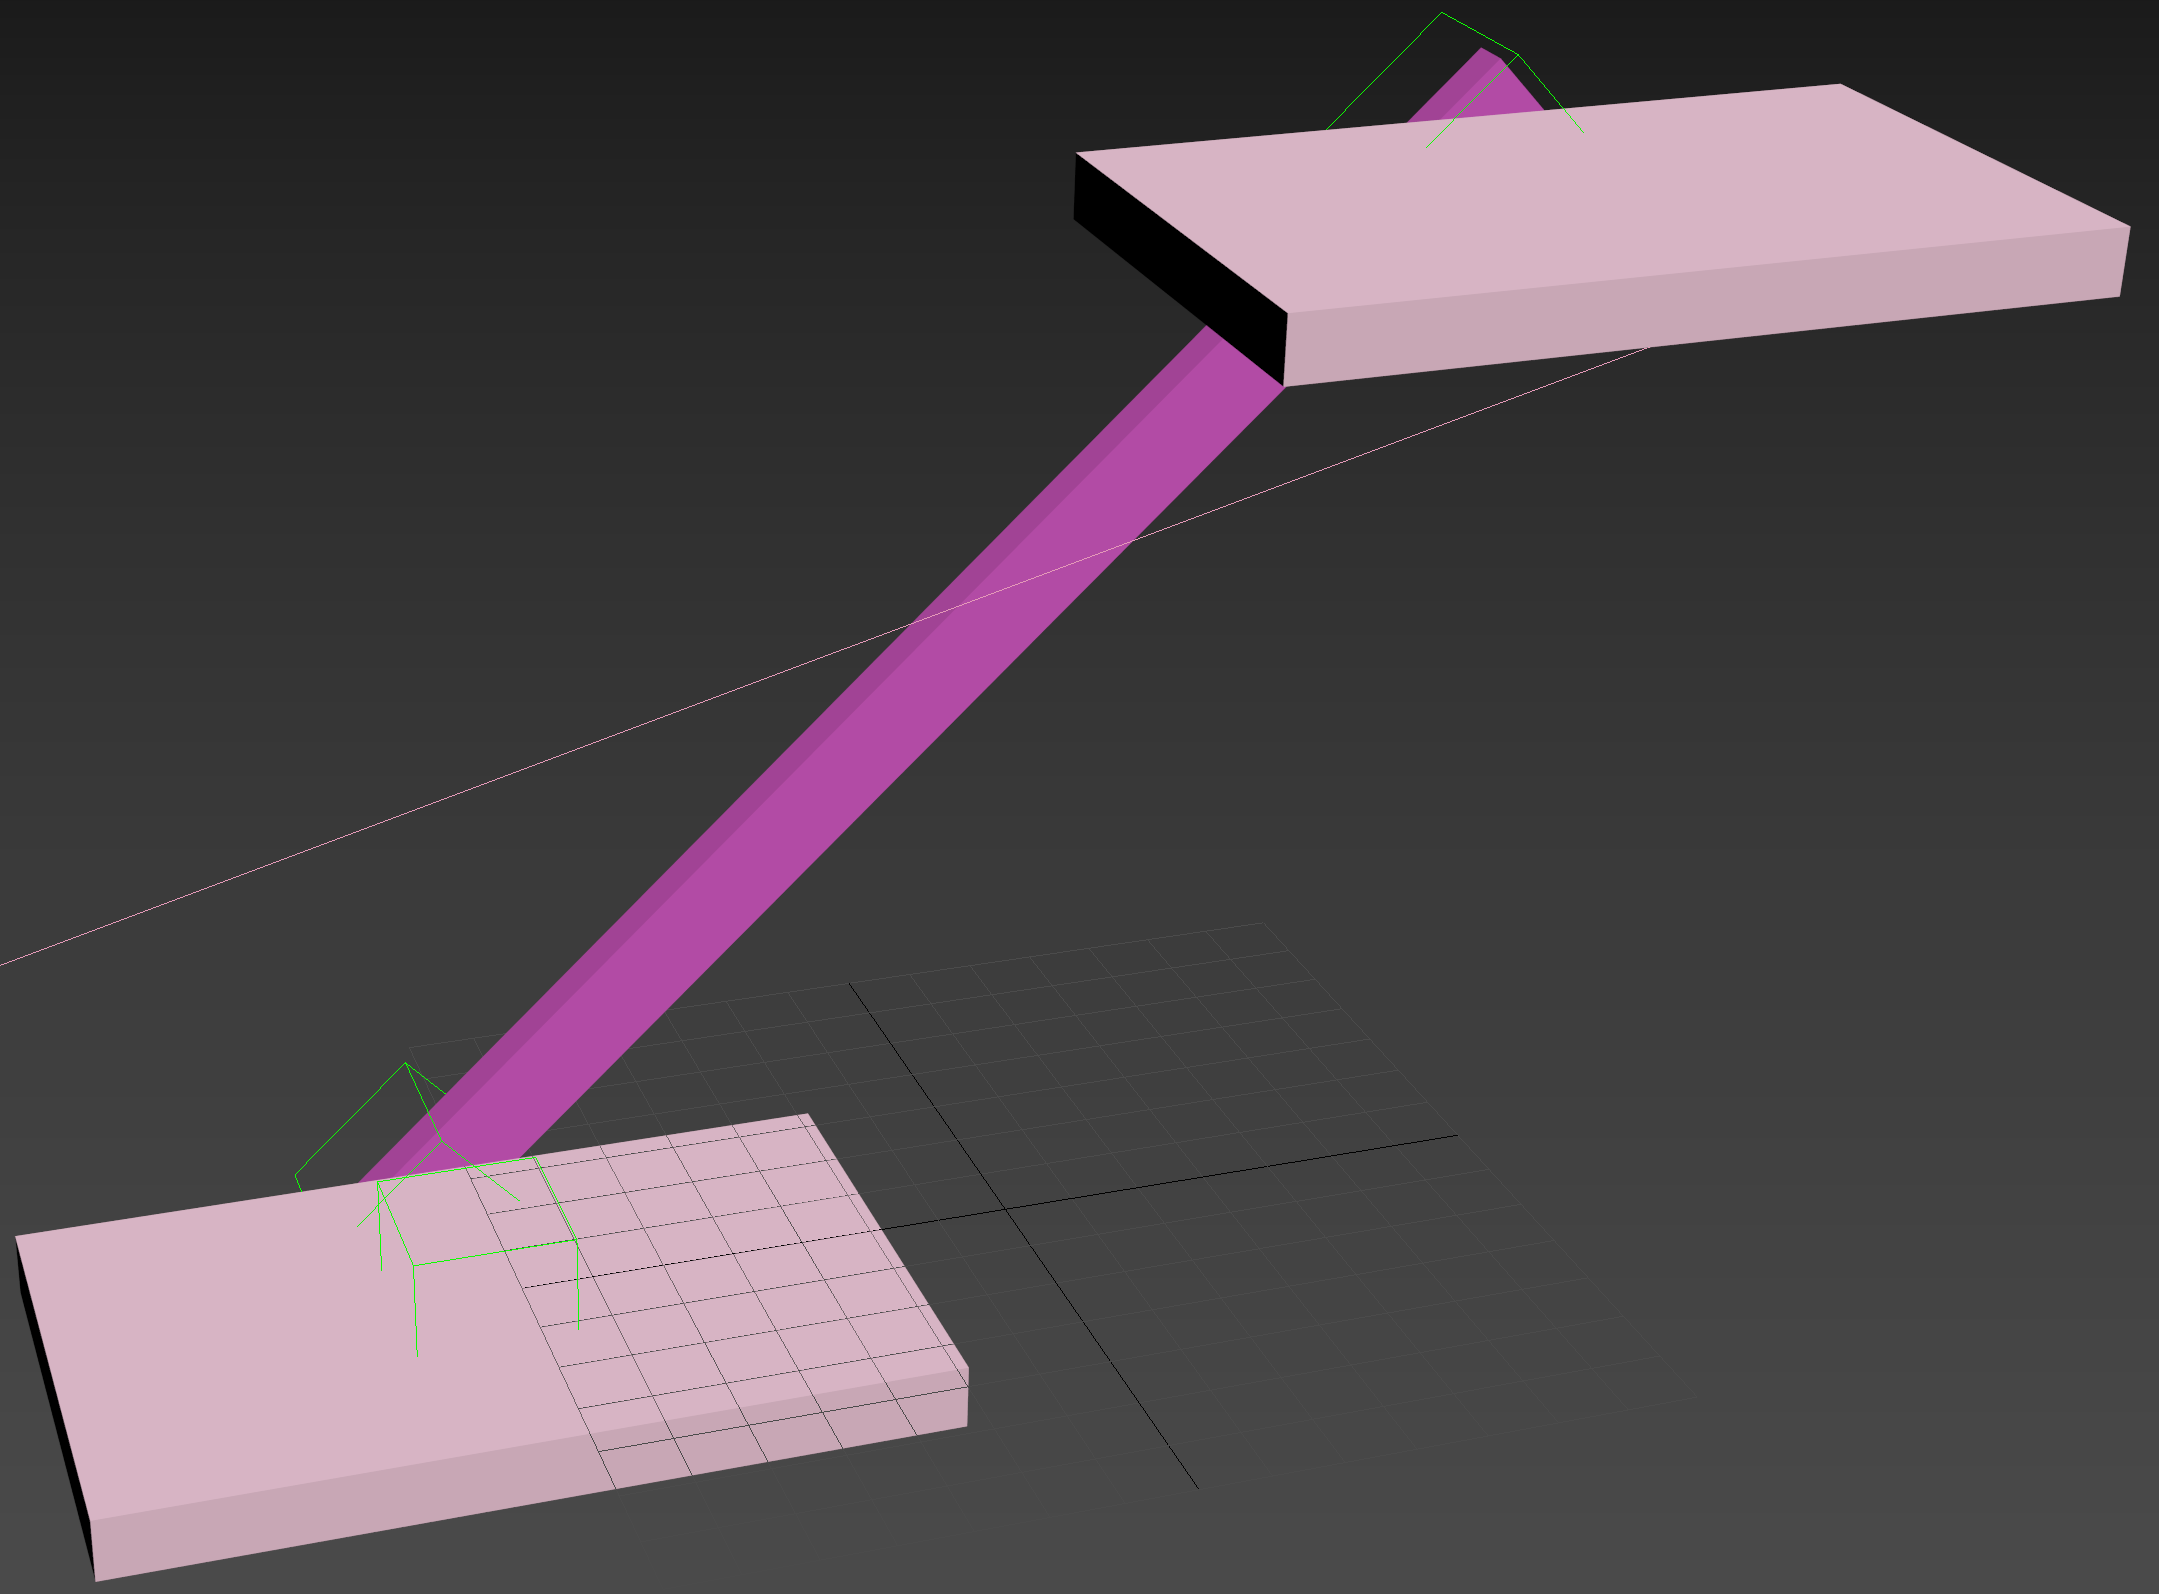
\includegraphics[width=0.6\textwidth]{imagenes/grua/grua.png}
    \caption{Forma final de la grúa.}
 \end{figure}

Los \textit{keyframes} de la grúa, más concretamente del brazo que gira, son:

\begin{itemize}
    \item \textbf{Instante 90: }Se encuentra en su posición inicial.
    \item \textbf{Instante 125: }El brazo ha girado y las plataformas han cambiado de posición, estando arriba la de abajo y viceversa.
\end{itemize}

\bigskip

La curva de animación para el brazo es:

% curva
\begin{figure}[H]
    \centering
    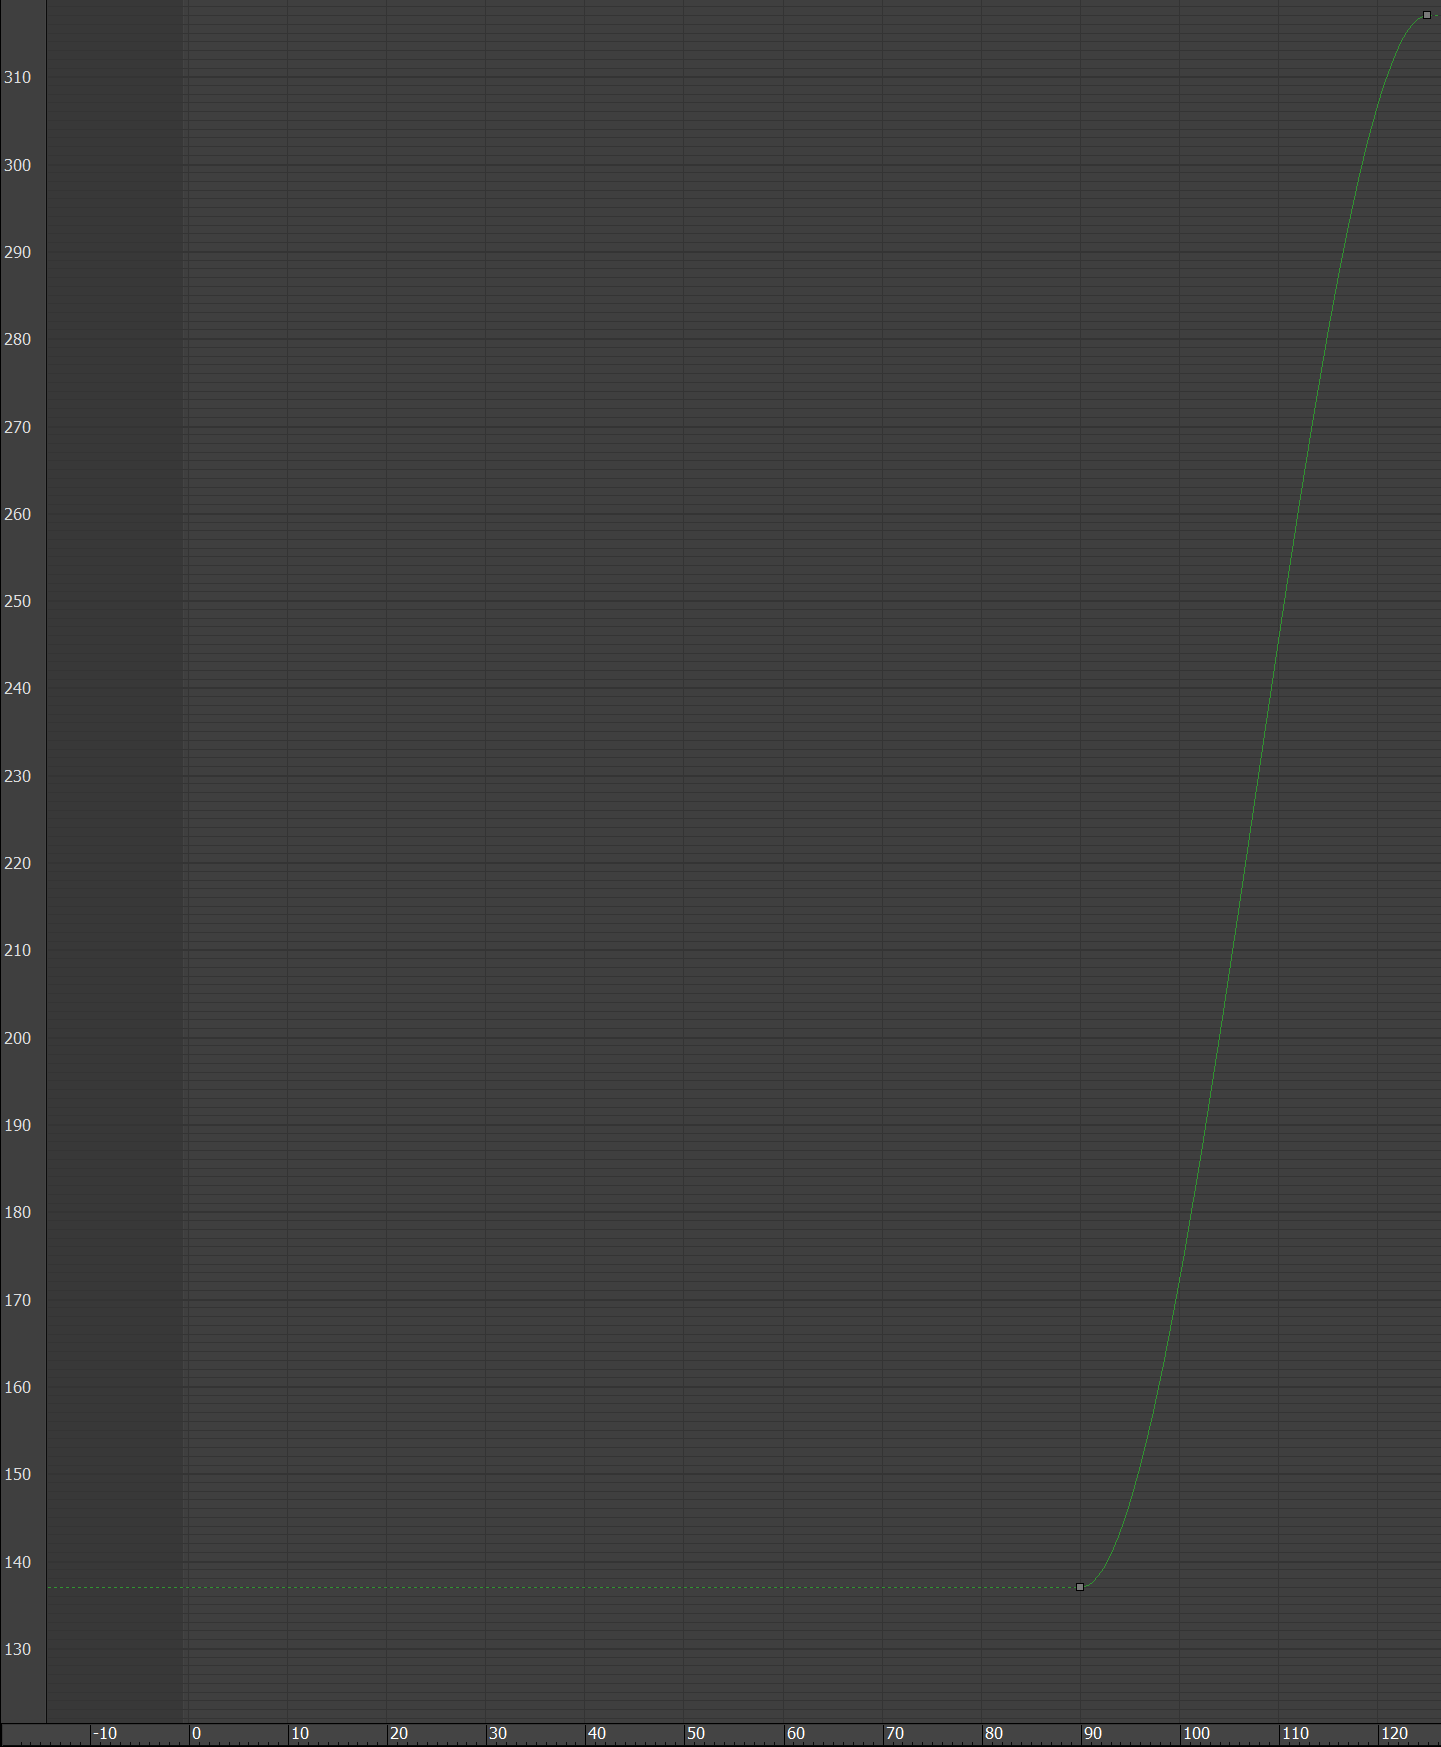
\includegraphics[width=0.5\textwidth]{imagenes/grua/rotY.png}
    \caption{Curva que representa la rotación en eje Y con respecto al tiempo.}
 \end{figure}

He vuelto a elegir una forma \textit{Slow-in/Slow-out} debido a que me parecía más realista que un motor tarde unas décimas de segundo en alcanzar la velocidad y también que requiera un tiempo en desacelerar.

\bigskip

Y los fotogramas más importantes después de haber hecho todo esto son:

% foto de los fotogramas mas imporantes.
\begin{figure}[H]
    \centering
\begin{subfigure}[t]{0.48\textwidth}
    \centering
    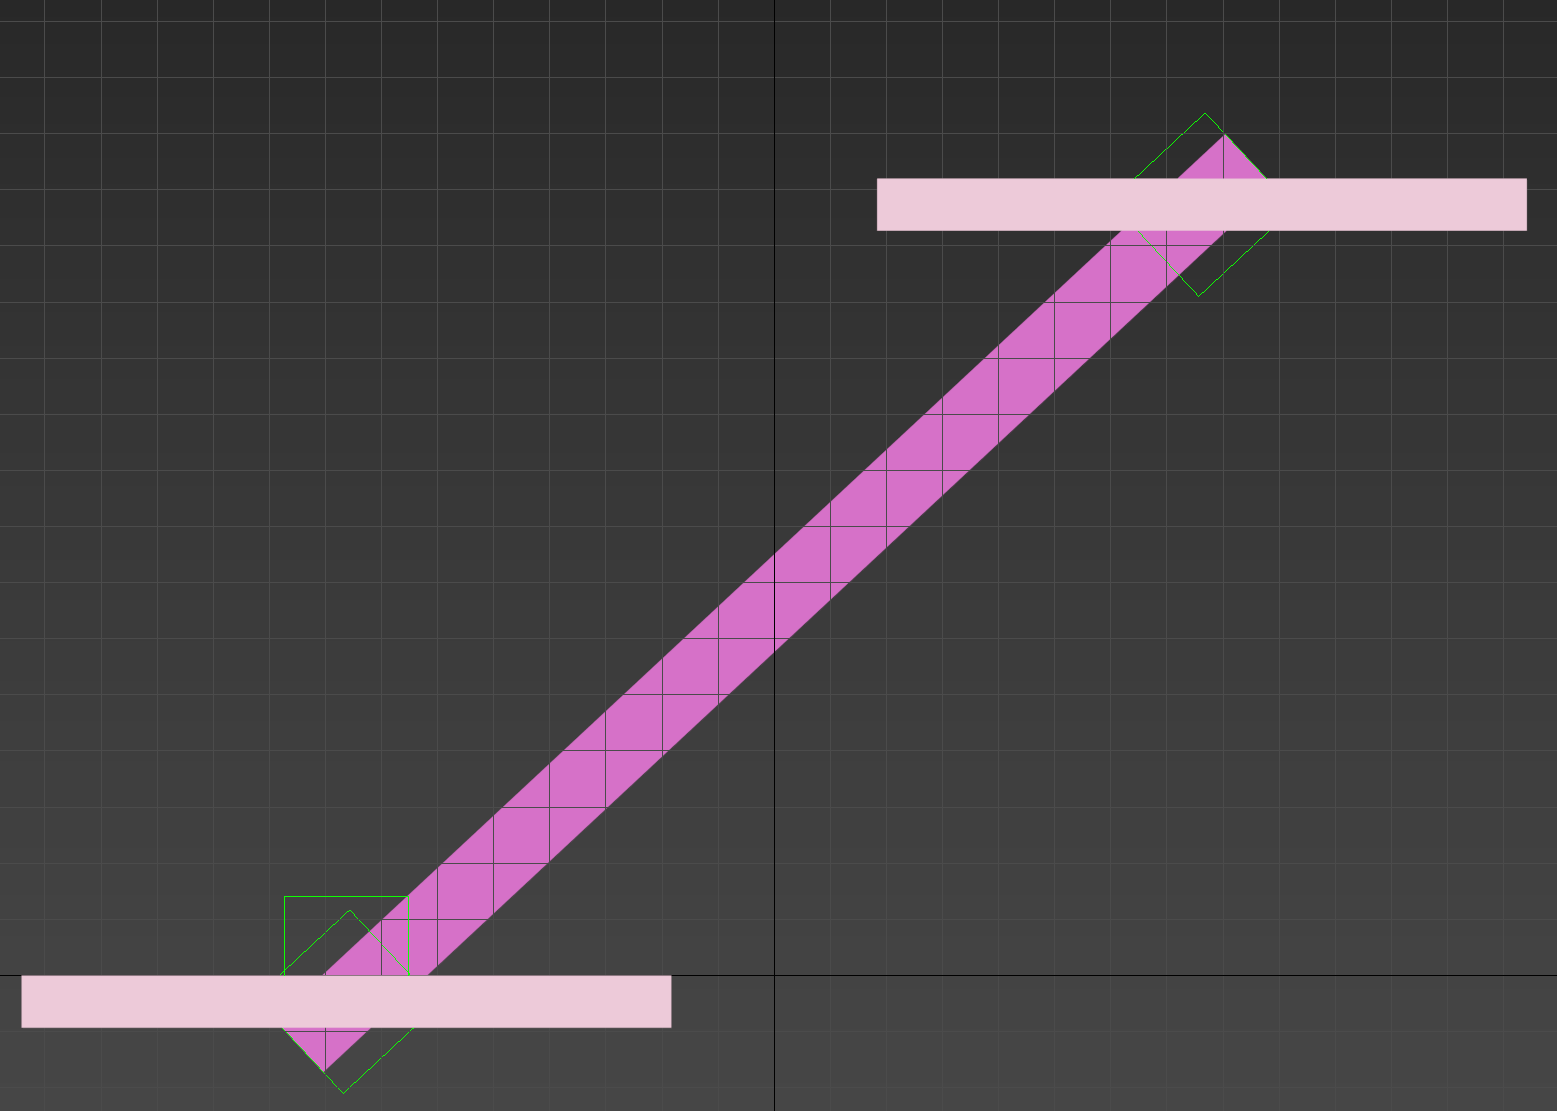
\includegraphics[width=\textwidth]{imagenes/grua/keyframes/90.png}
    \caption{Grúa en el instante 90 y anterior.}
 \end{subfigure}
\hfill
 \begin{subfigure}[t]{0.48\textwidth}
    \centering
    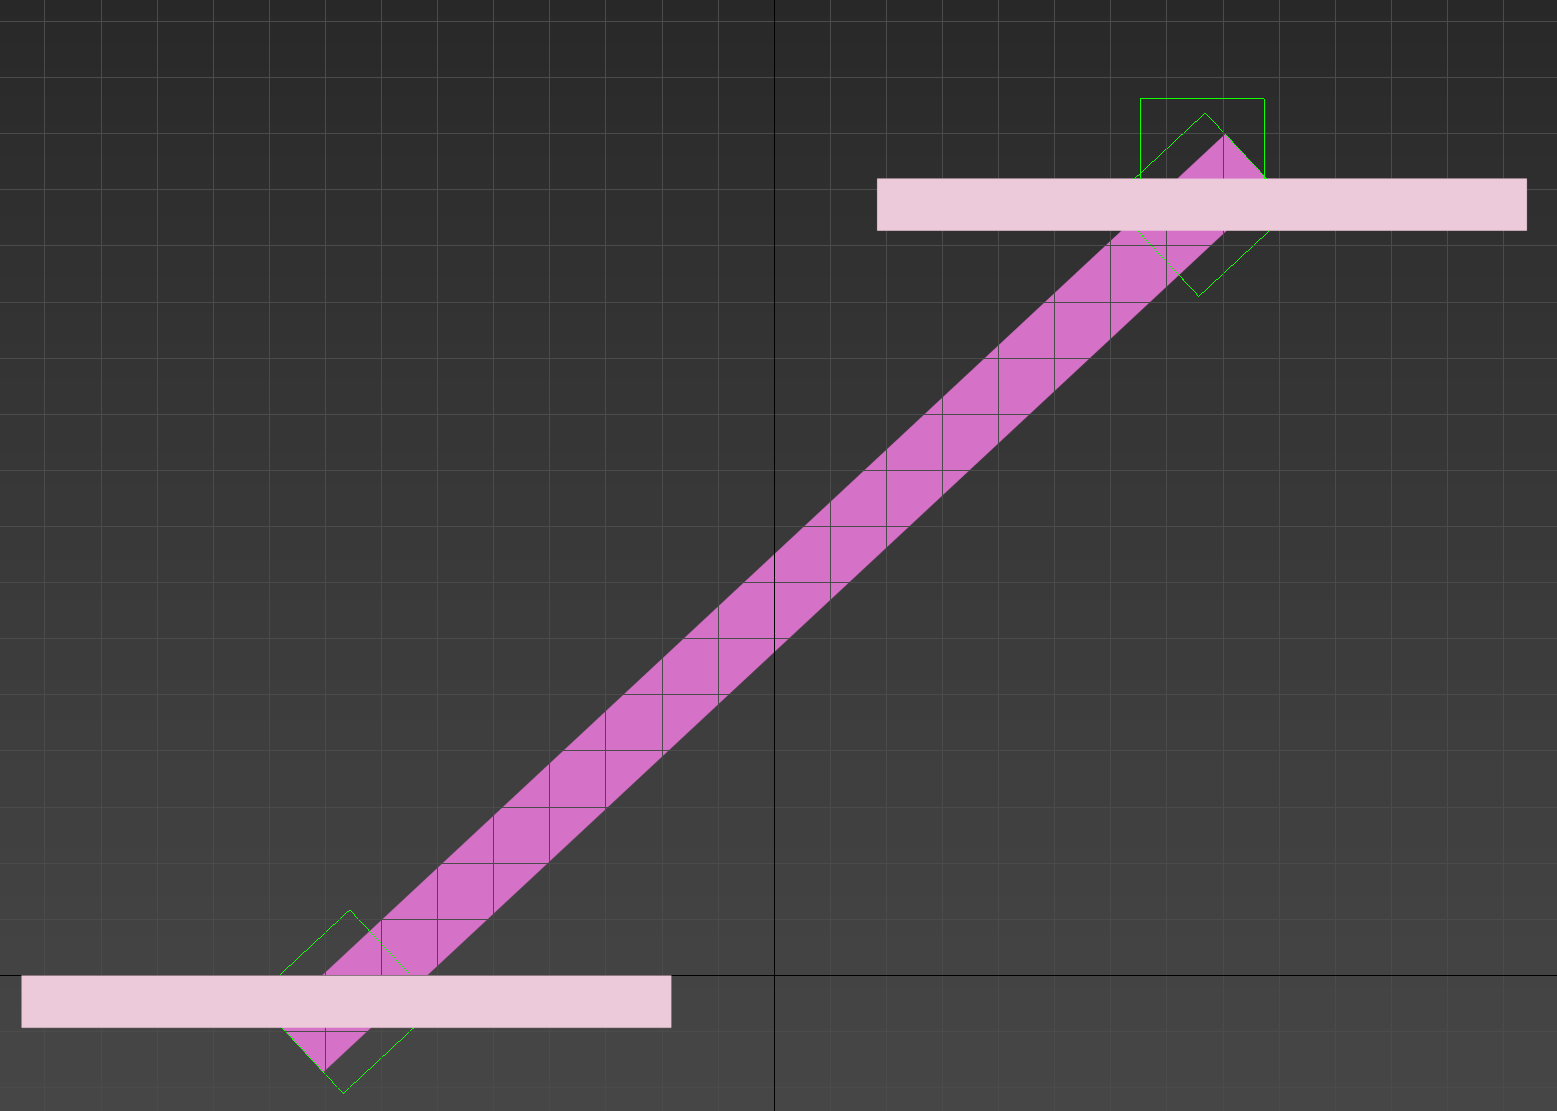
\includegraphics[width=\textwidth]{imagenes/grua/keyframes/125.png}
    \caption{Grúa en el instante 125 y siguientes.}
 \end{subfigure}
 \caption{\textit{Keyframes} de la grúa.}
\end{figure}
\newpage

\section{Coche}

La composición del coche es muy similar al usado en la práctica 2, con la misma jerarquía, pero los cilindros de las ruedas tienen menos aristas, para acentuar el efecto de movimiento de las ruedas. Además, como se pide que la espada deba mirar a la parte superior del vehículo, he usado un \textit{Dummy} para que mire correctamente. Si bien se podría haber hecho con el cubo de arriba, me ha parecido más correcto hacer esto, ya que no va a mirar al centro del coche, sino a la parte trasera.

\bigskip

Voy a dividir cada restricción, incluyendo la de la espada, en subsecciones:


% ACTUALIZAR ESTA SECCION SI SE CAMBIA EL LUNES ALGO
% QUIZAS RESCRIBIR ALGUNAS FRASES, QUE SON RARAS
\subsection{Configuración de la espada para que gire}

Para que la espada mire, es necesario utilizar la restricción \textit{LookAt Constraint}, junto al \textit{Select LookAt Axis} en el eje Z, para que funcione correctamente. Con esto hecho, hace falta seleccionar los \textit{Targets}, que en mi caso son dos:

\begin{itemize}
    \item Un primer \textit{Dummy} que siempre se encuentra encima de la espada para que esta apunte hacia arriba en un primer momento. Este objeto tiene una restricción \textit{Link}, que está unida a las manos y la plataforma, haciendo que así siga siempre a la espada.
    
    Además, he bloqueado la herencia de rotación y escalado, para que sea muy similar al \textit{Position Constraint}, pero más flexible en términos de ajustar el \textit{dummy} a la escena.

    Esto se puede hacer yendo a \textit{Hierarchy} $\rightarrow$ \textit{Link Info}:

    \begin{figure}[H]
        \centering
       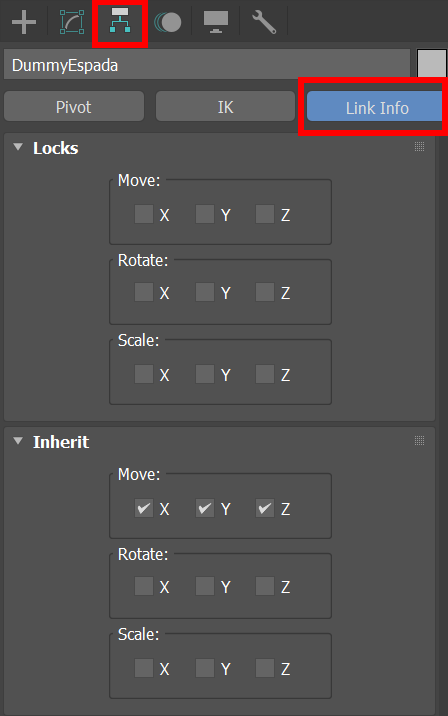
\includegraphics[width=0.35\textwidth]{imagenes/espada/dummyTopHierarchy.png}
       \caption{Menú para bloquear canales.}
    \end{figure}

    \item El segundo \textit{Dummy} es el comentado anteriormente, uno que se encuentra en la parte trasera superior del coche.
\end{itemize}

Con esto hecho, solo falta hacer una transición suave de un \textit{target} a otro. Entonces, los instantes referentes a esta restricción son:

\begin{itemize}
    \item \textbf{Instante 125: }La espada sigue mirando al \textit{dummy} que tiene justo encima.
    \item \textbf{Instante 150: }La espada ahora está mirando completamente hacia el \textit{dummy} del coche.
\end{itemize}

Las curvas de animación de la restricción son:

% curvas de la restricción
\begin{figure}[H]
    \centering
   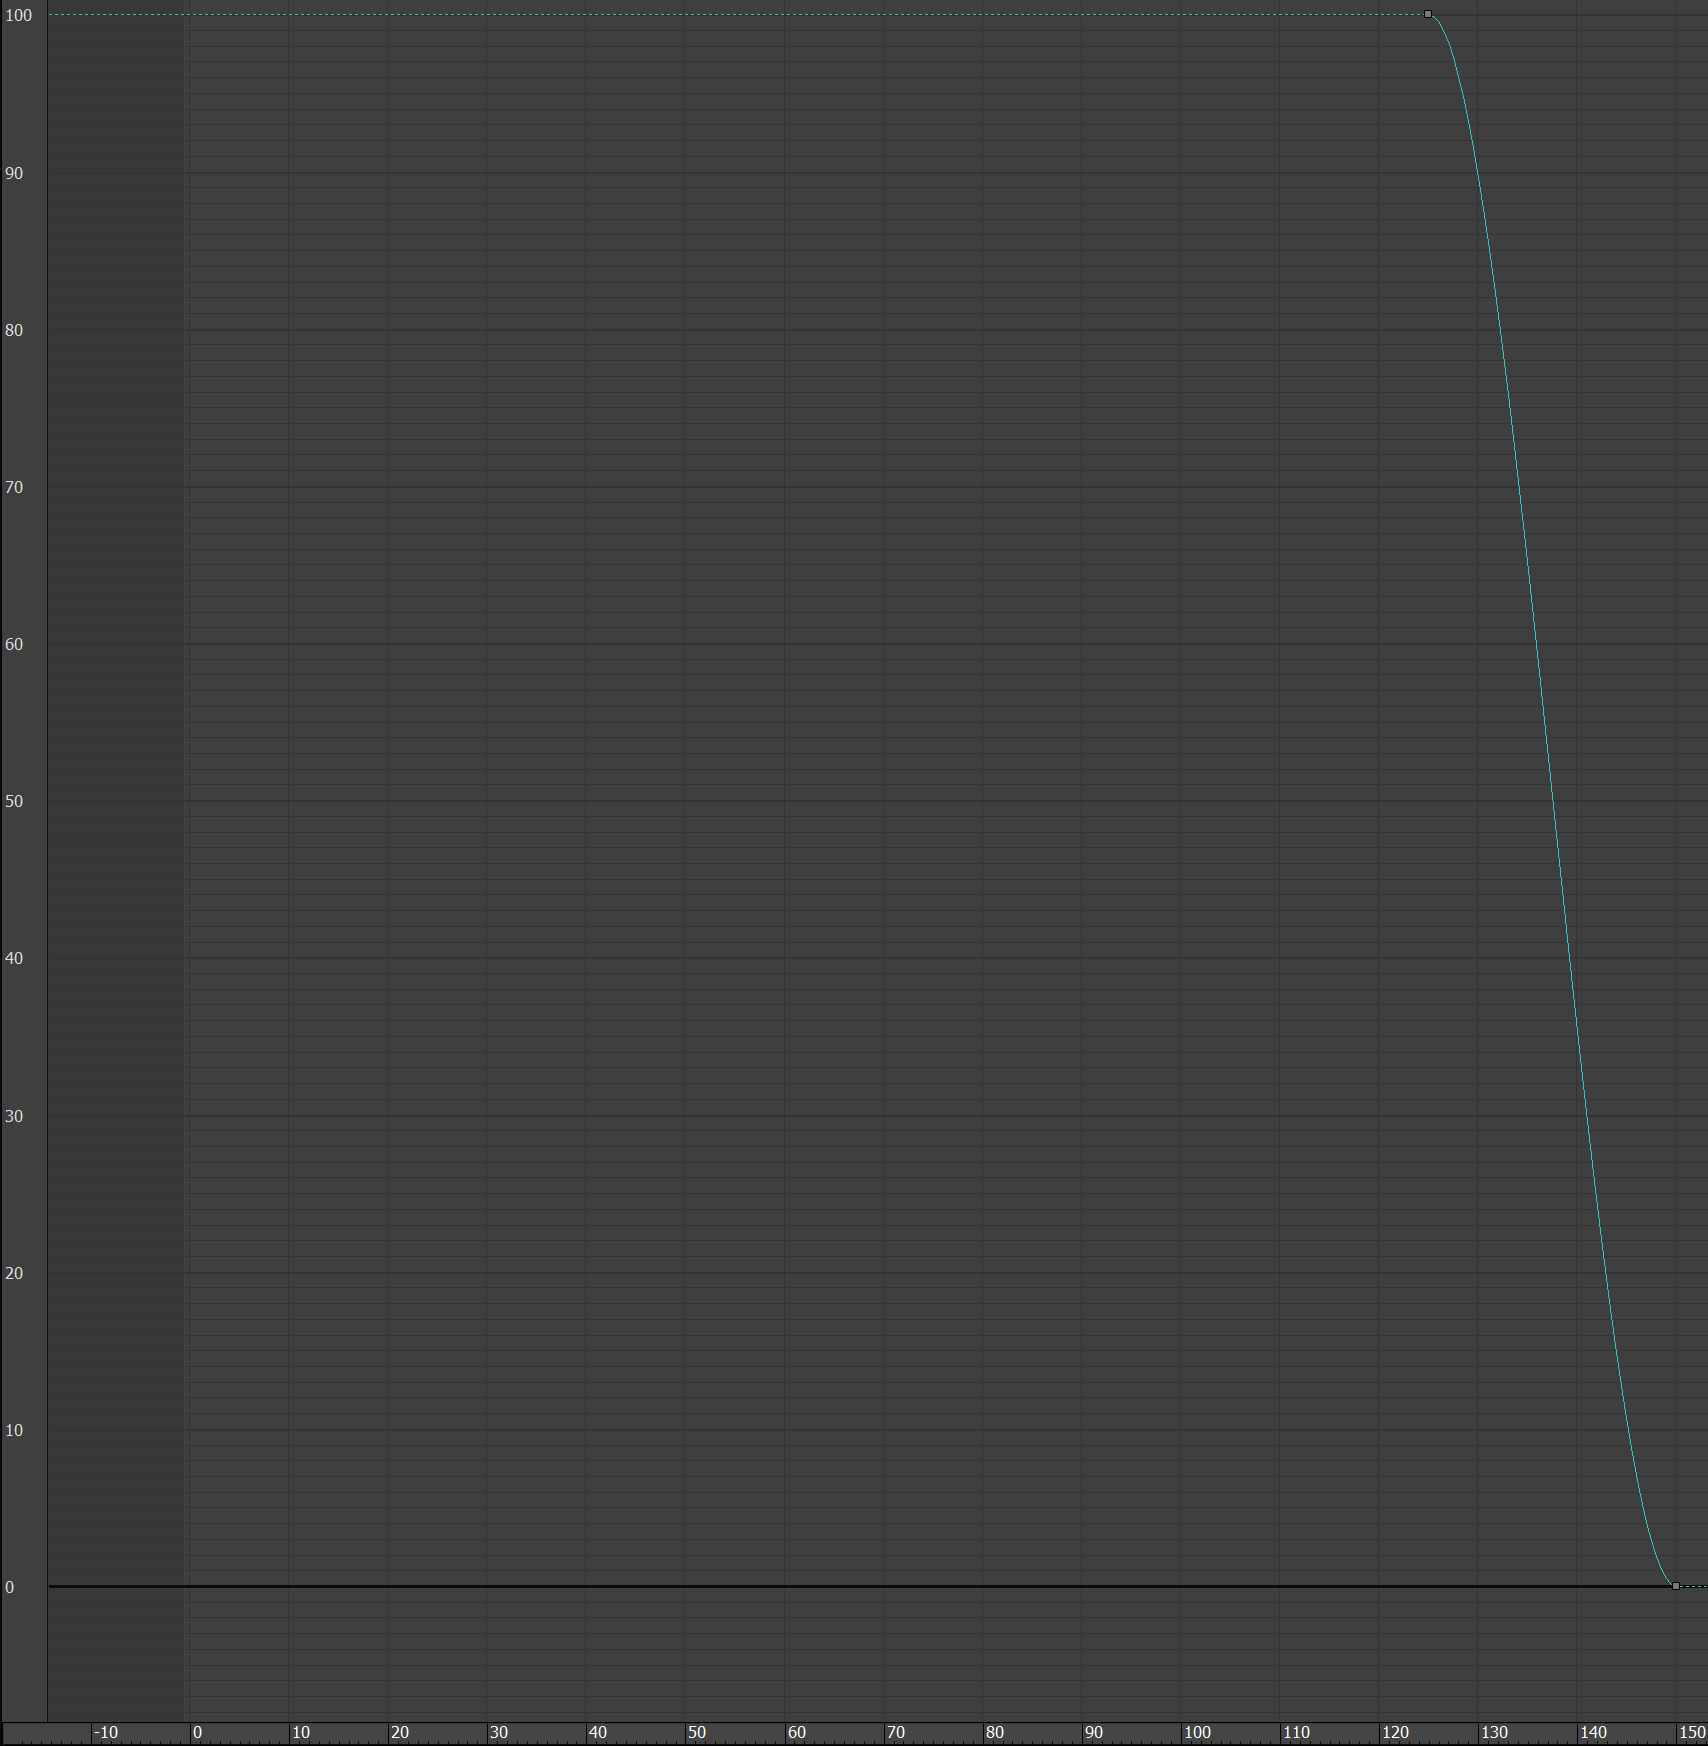
\includegraphics[width=0.6\textwidth]{imagenes/espada/lookat0.png}
   \caption{Curva usada para realizar el cambio de pesos en la restricción en el objetivo del \textit{dummy}.}
\end{figure}

\begin{figure}[H]
    \centering
   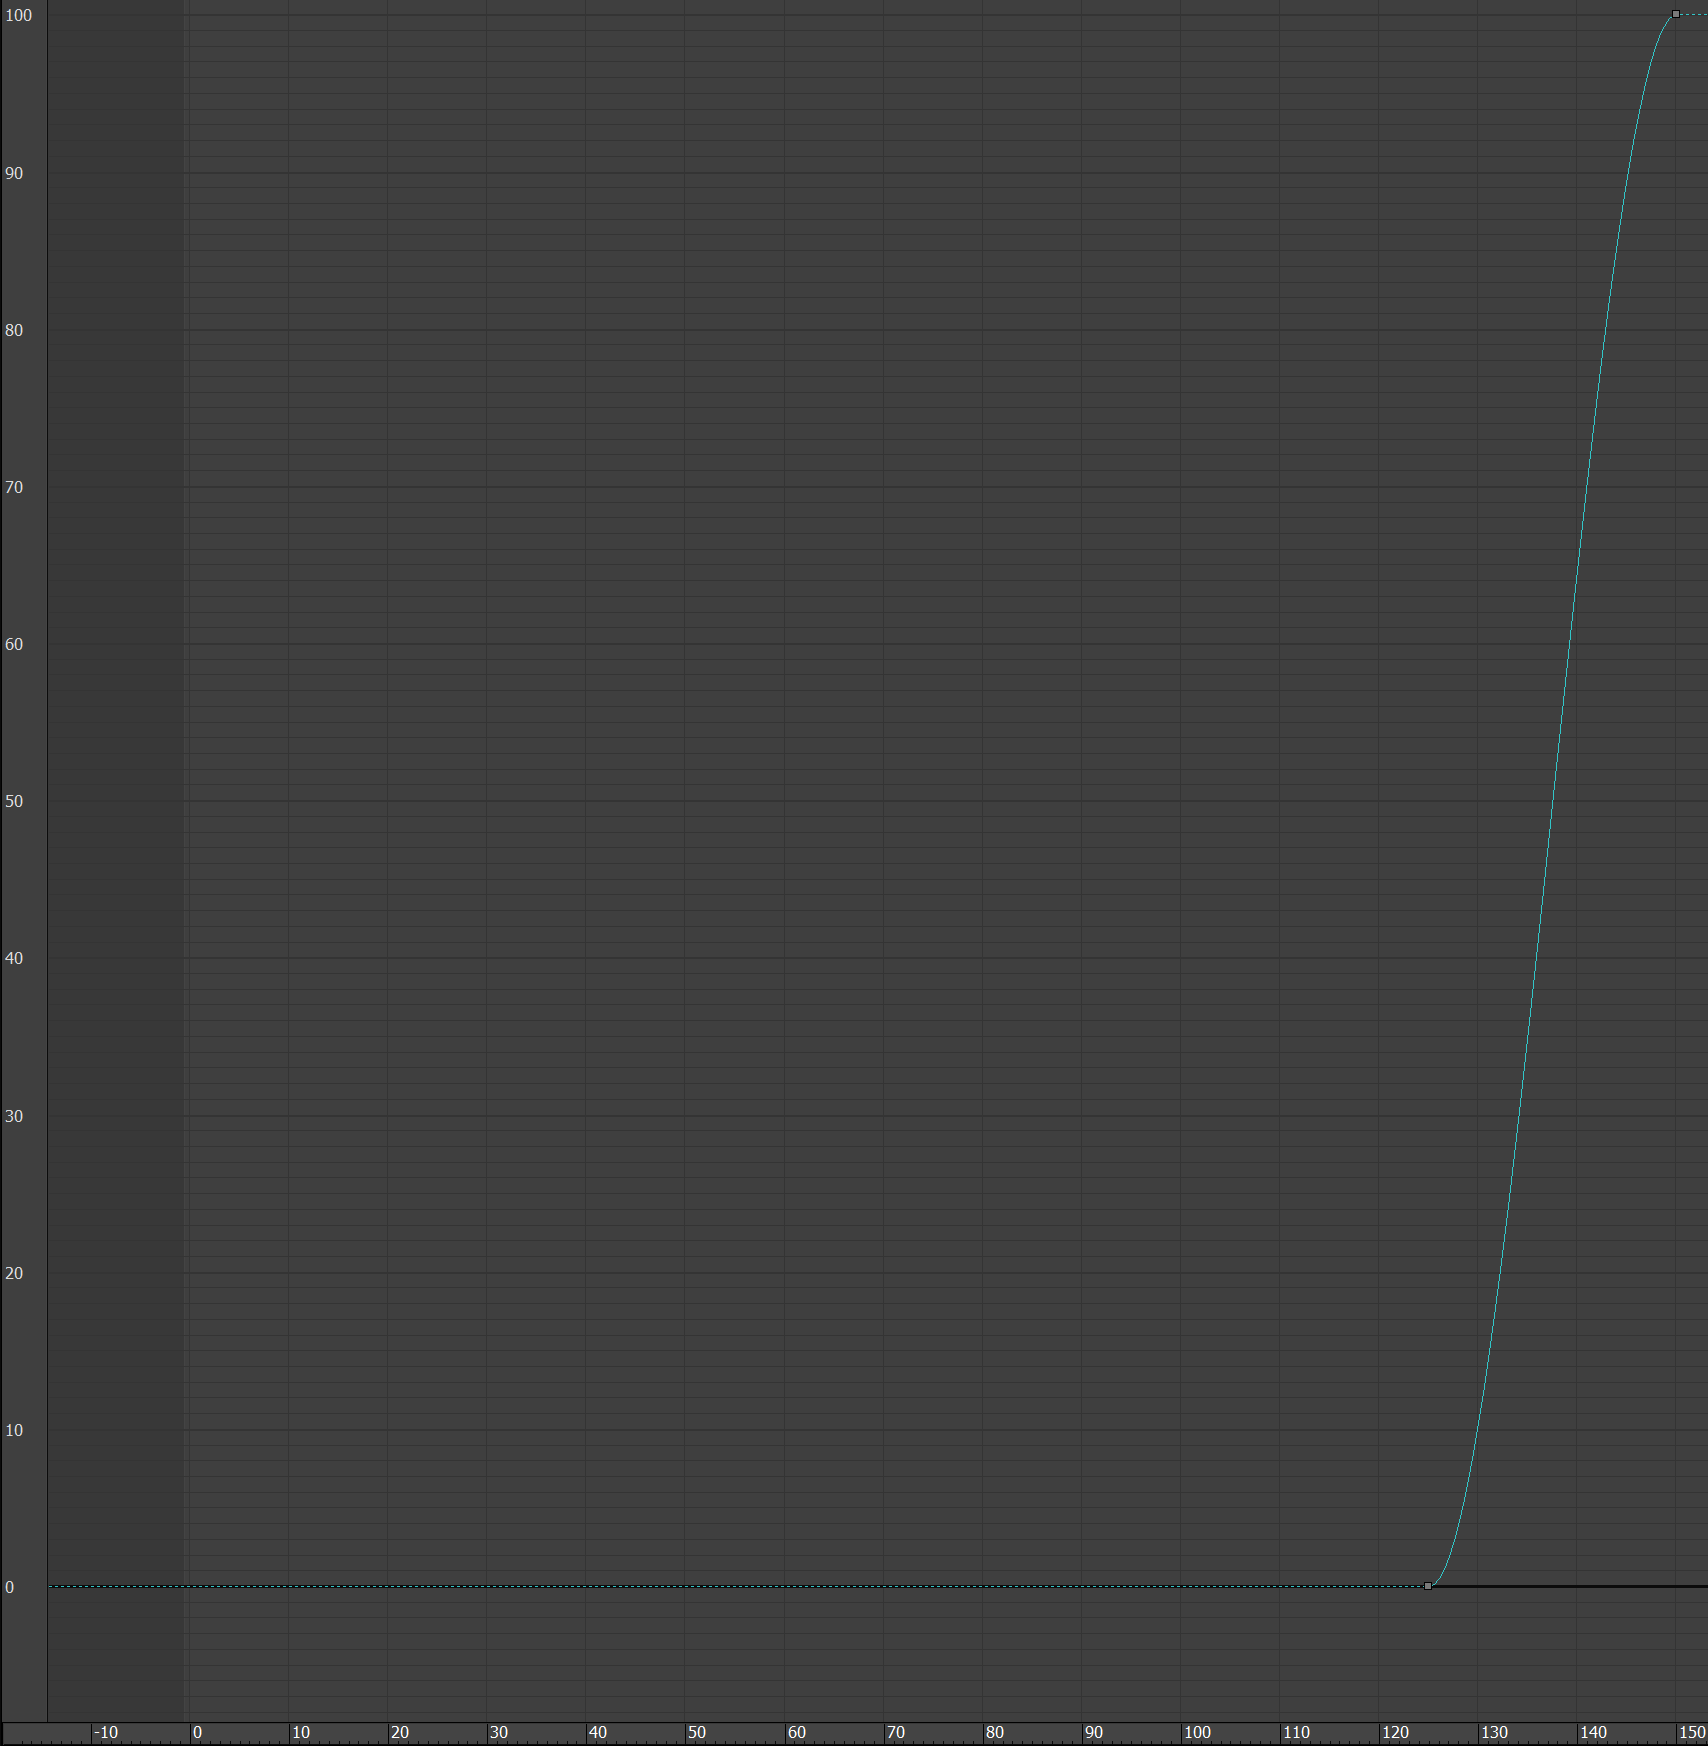
\includegraphics[width=0.6\textwidth]{imagenes/espada/lookat1.png}
   \caption{Curva usada para realizar el cambio de pesos en la restricción en el objetivo del \textit{dummy} del coche.}
\end{figure}

Como se puede ver, he utilizado la forma de la curva \textit{Slow-in/Slow-out}, ya que probando otros tipos no me han parecido del todo realistas.

\bigskip

\newpage

Además, la configuración final del \textit{LookAt Constraint} es:

\begin{figure}[H]
    \centering
   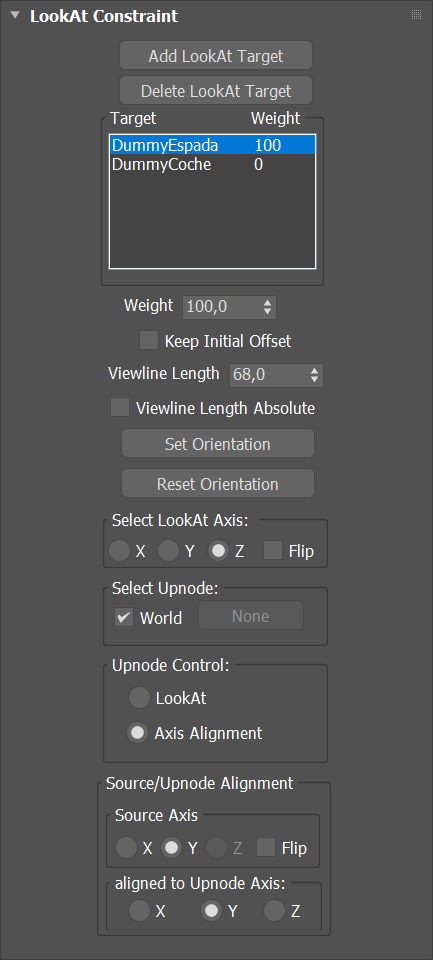
\includegraphics[width=0.3\textwidth]{imagenes/espada/lookatconfig.png}
   \caption{Configuración final del \textit{LookAt Constraint} en el espada.}
\end{figure}

% rescribir esta parte, digo mucho en mi caso
\subsection{Seguimiento de la curva}

Lo primero que hay que hacer es generar un spline que será usado por el coche para realizar la ruta.

\begin{figure}[H]
    \centering
   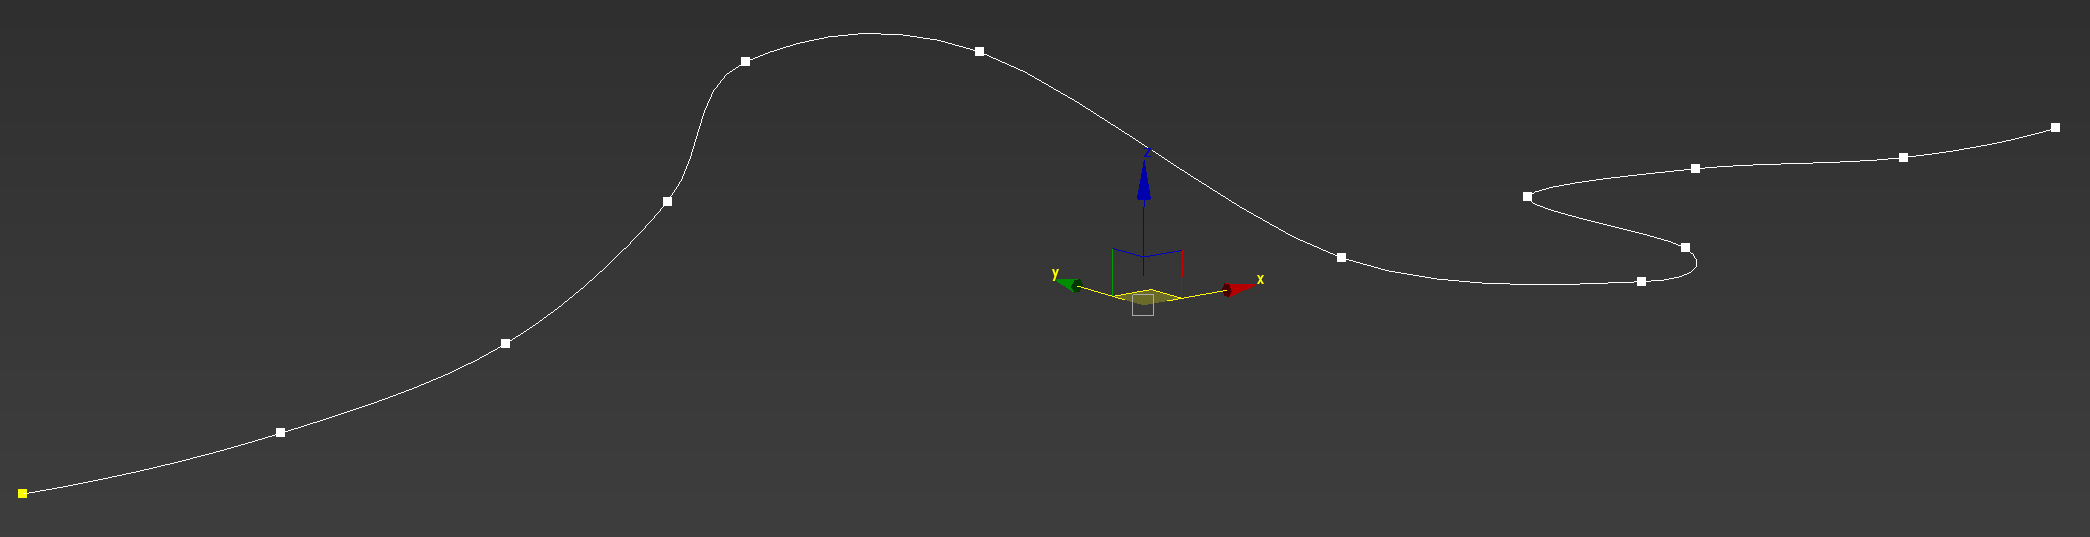
\includegraphics[width=0.6\textwidth]{imagenes/spline/spline.png}
   \caption{Forma que tiene el spline, se puede ver que sube y baja también.}
\end{figure}

Una vez generado, es necesario ponerle al coche la restricción \textit{Path Constraint} con el \textit{Path} creado anteriormente. En mi caso he decidido ponérselo al padre de la jerarquía, que es el cubo inferior. Además, hay que habilitar la opción \textit{Follow} para que el coche lo siga y deshabilitar la opción \textit{Loop} para que no siga infinitamente.

\bigskip

Una vez hecho esto, simplemente es necesario modificar los \textit{keyframes} de inicio y final para que vaya más lento, que en mi caso han sido los instantes \textbf{150} y \textbf{300}.

\bigskip

Tras hacer esto, se puede ver como el coche se mueve siguiendo el spline de manera correcta.

\bigskip

\newpage

La curva de animación es:

\begin{figure}[H]
    \centering
   
\includegraphics[width=0.5\textwidth]{imagenes/coche/pathConstraint.png}
   \caption{Curva del \textit{Path Constraint} que representa la posición del coche en el spline con respecto al tiempo.}
\end{figure}

Tras intentar de distintas formas modificar la forma de la curva del \textit{Path Constraint}, me ha sido imposible modificarla, por lo que la curva tiene forma lineal, que no es del todo realista, ya que un coche necesita un tiempo para acelerar y frenar.

\subsection{Movimiento de las ruedas}

Para hacer el movimiento de las ruedas, he usado \textit{Wire Parameter}, he seleccionado la rotación en el eje Y de una de ellas y la he unido a la caja del coche que tiene el \textit{Path Constraint}, más concretamente al porcentaje que ha recorrido en el spline. Esto lo he hecho así, ya que si hubiese elegido la posición en el eje X, al estar el coche en una zona que no fuera paralela a dicho eje, las ruedas girarían menos.

\bigskip

% QUIZAS COMPROBAR ESTO, QUE PUEDE SER QUE CAMBIE
En cuanto a la rotación, la he multiplicado por un factor de \rotFactor para que el giro realizado sea natural y más rápido de lo que tiene por defecto.

% foto del menu wire parameter
\begin{figure}[H]
    \centering
   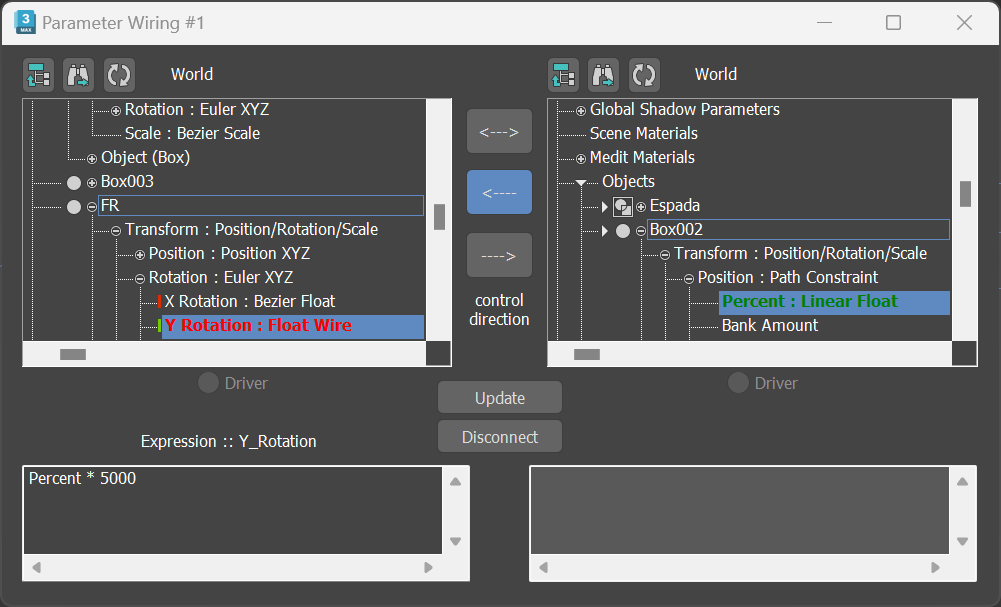
\includegraphics[width=0.6\textwidth]{imagenes/coche/wireFR.png}
   \caption{Menú con la configuración de la rueda.}
\end{figure}

Para simplificar futuros cambios en el factor de rotación, he asignado la rotación de las demás ruedas en el eje Y con la que tiene el porcentaje del spline, así se puede cambiar solo una vez el parámetro. Además, las ruedas del lado izquierdo deben tener un factor de -1 aplicado, ya que estas ruedas están rotadas 180 grados en el eje Z, haciendo que si no se usase girasen en el sentido contrario.

\begin{figure}[H]
    \centering
   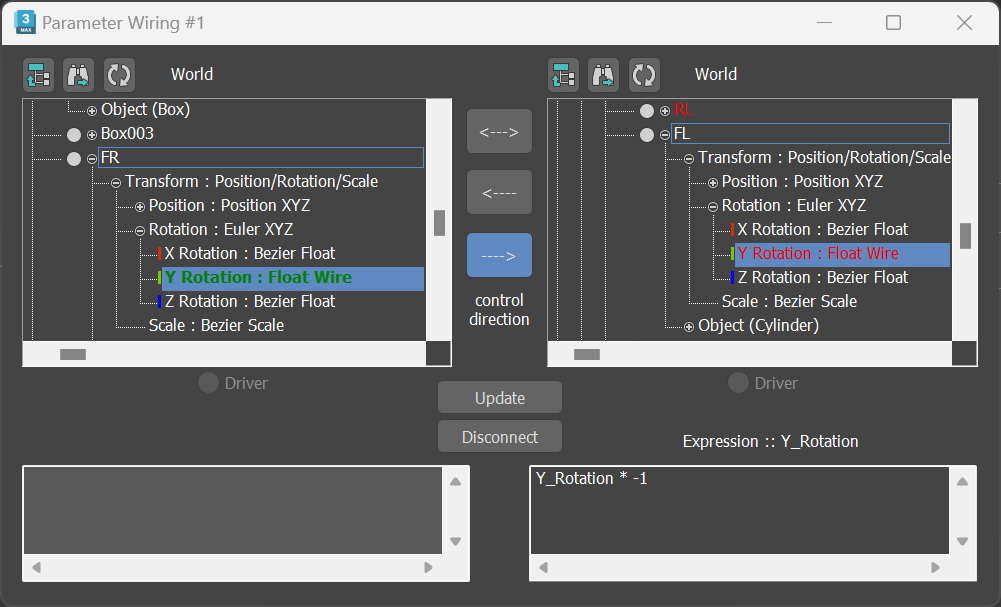
\includegraphics[width=0.6\textwidth]{imagenes/coche/wireFL.png}
   \caption{Ejemplo de la expresión utilizada para las ruedas de la izquierda.}
\end{figure}


Además, la configuración de la restricción es: 

\begin{figure}[H]
    \centering
   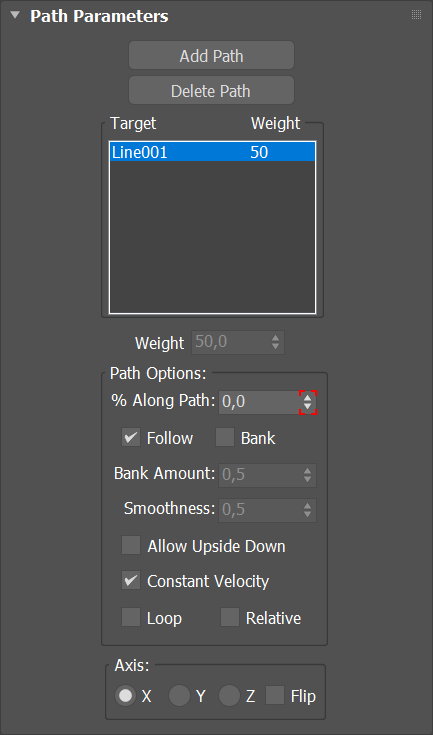
\includegraphics[width=0.3\textwidth]{imagenes/coche/config.png}
   \caption{Configuración del \textit{Path Constraint}.}
\end{figure}

\newpage

\subsection{Resultado final}

Los fotogramas más importantes relativos al coche son:

% fotos
\begin{figure}[H]
    \centering
    \begin{subfigure}[t]{0.48\textwidth}
        \centering
        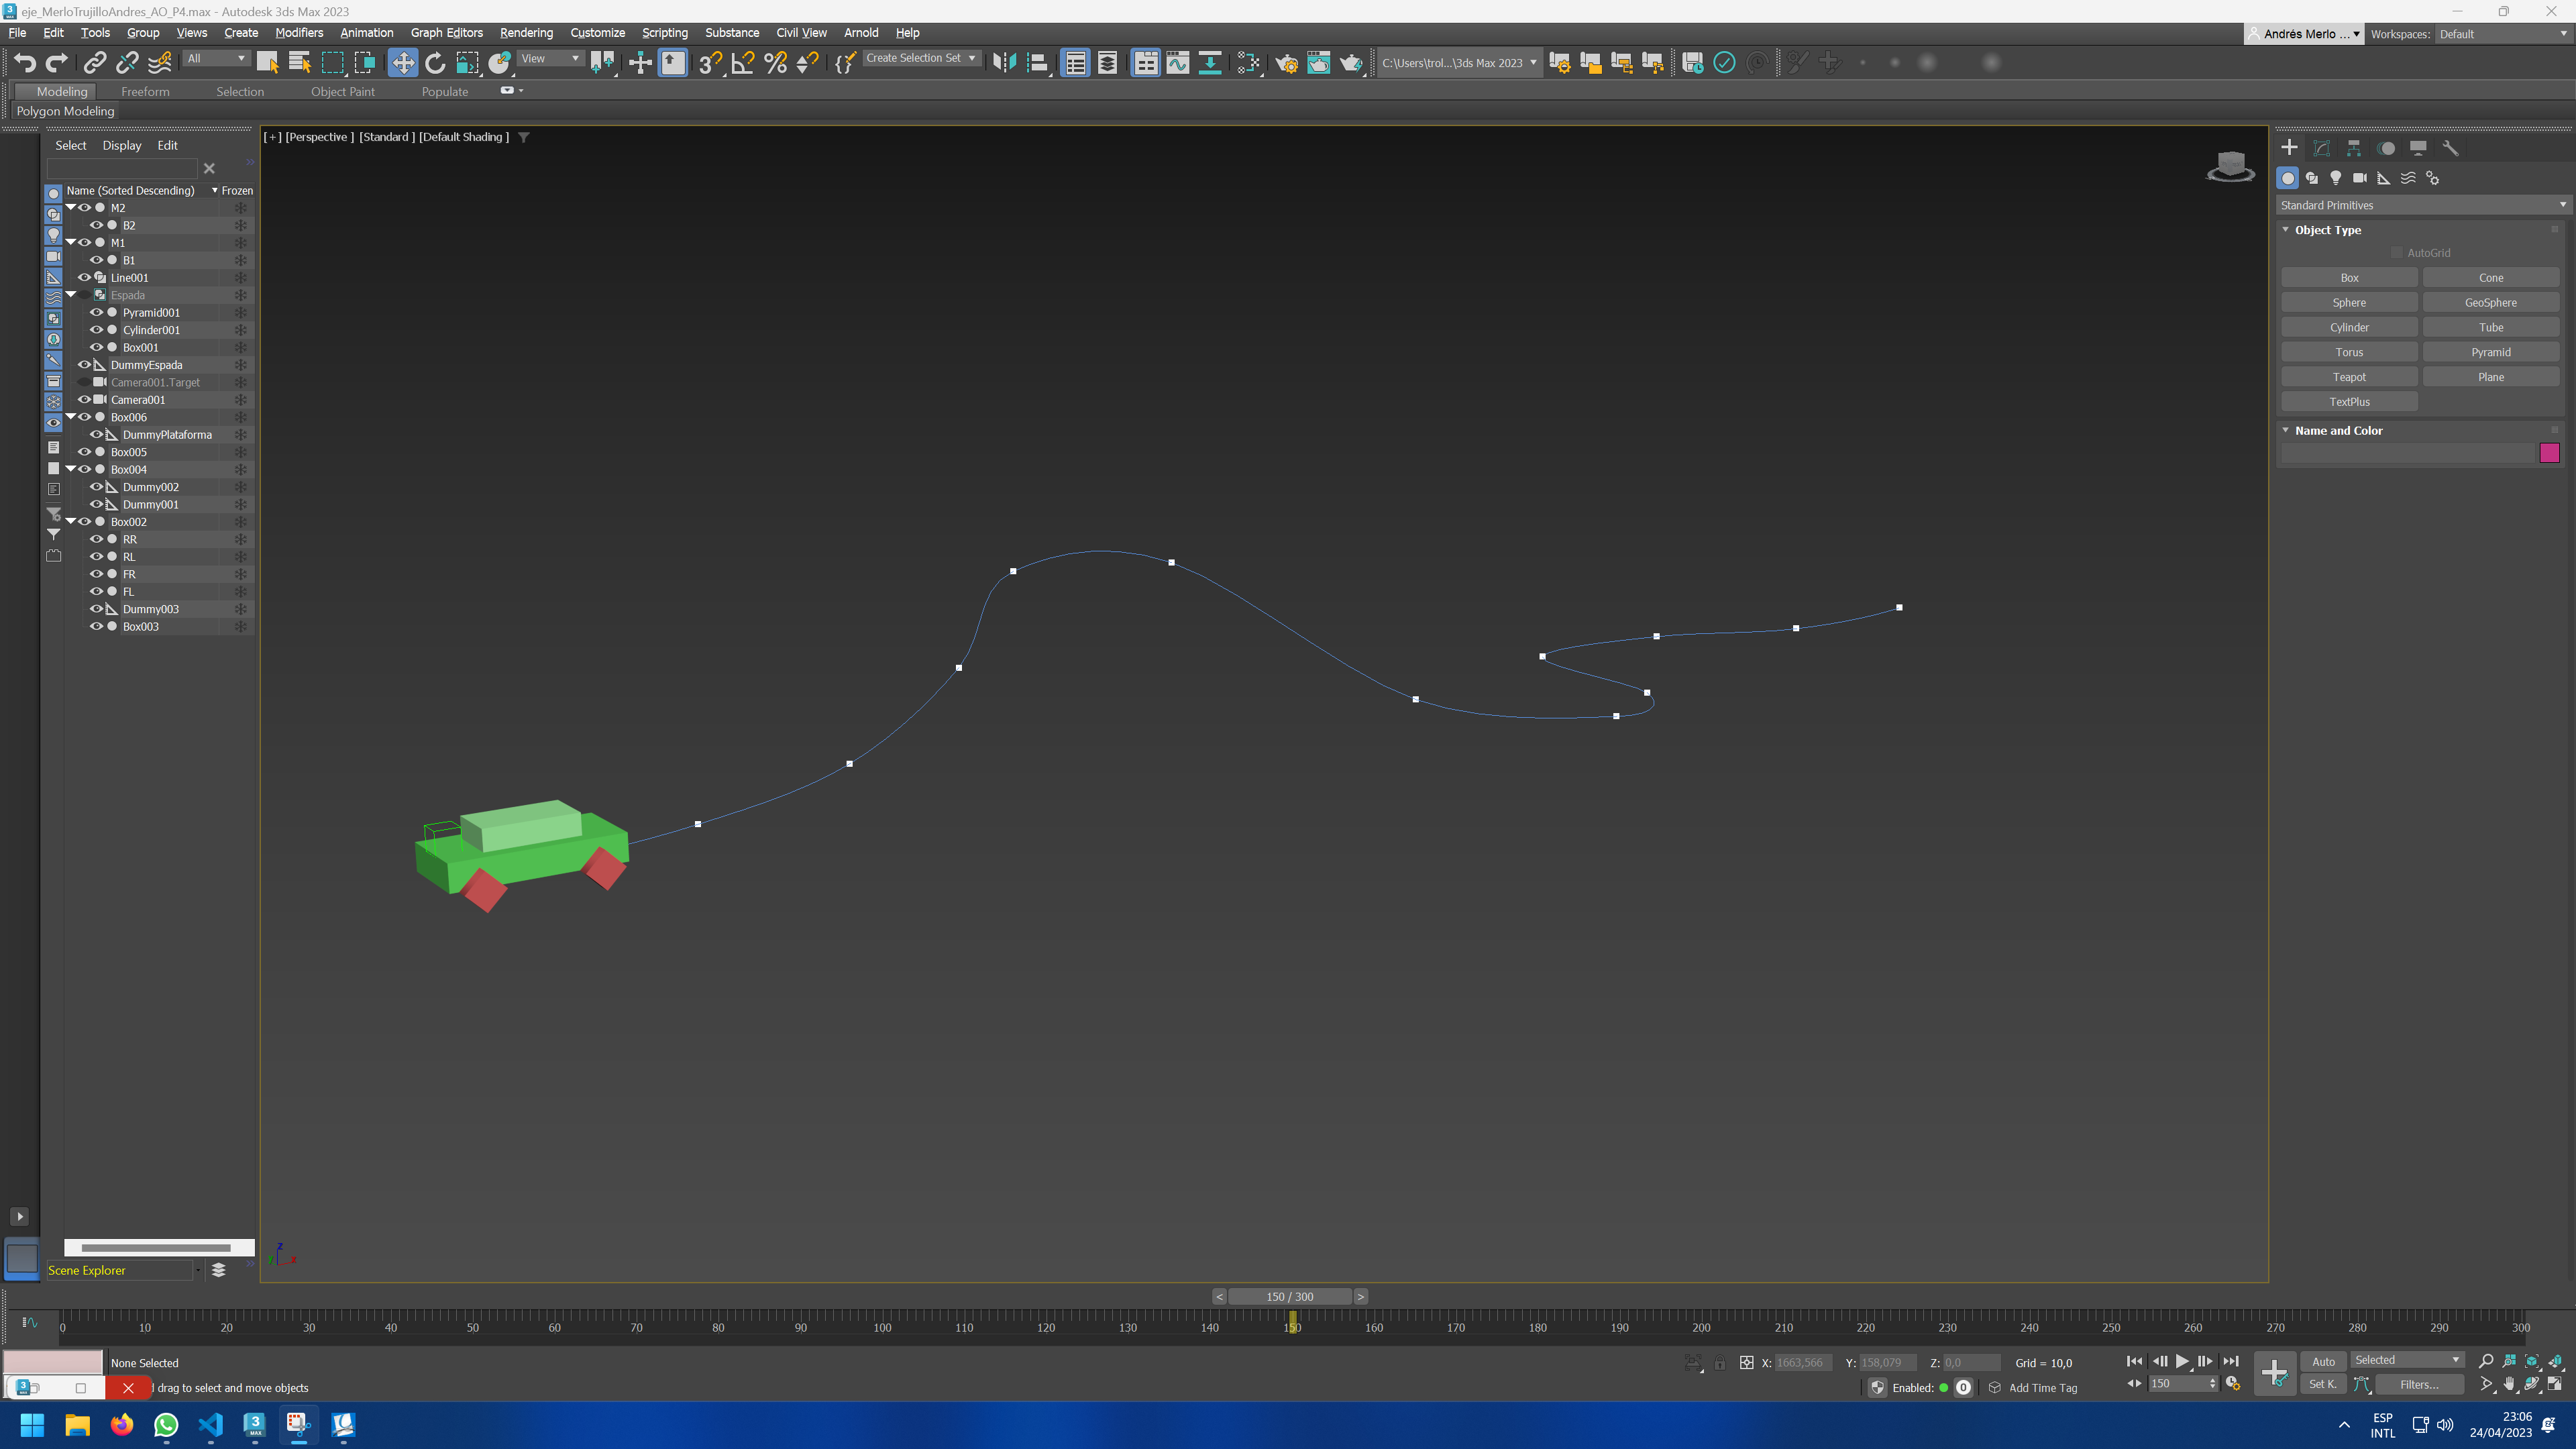
\includegraphics[width=\textwidth]{imagenes/coche/keyframes/150.png}
        \caption{Coche en el instante 150 y anteriores.}
    \end{subfigure}
    \hfill
    \begin{subfigure}[t]{0.48\textwidth}
        \centering
        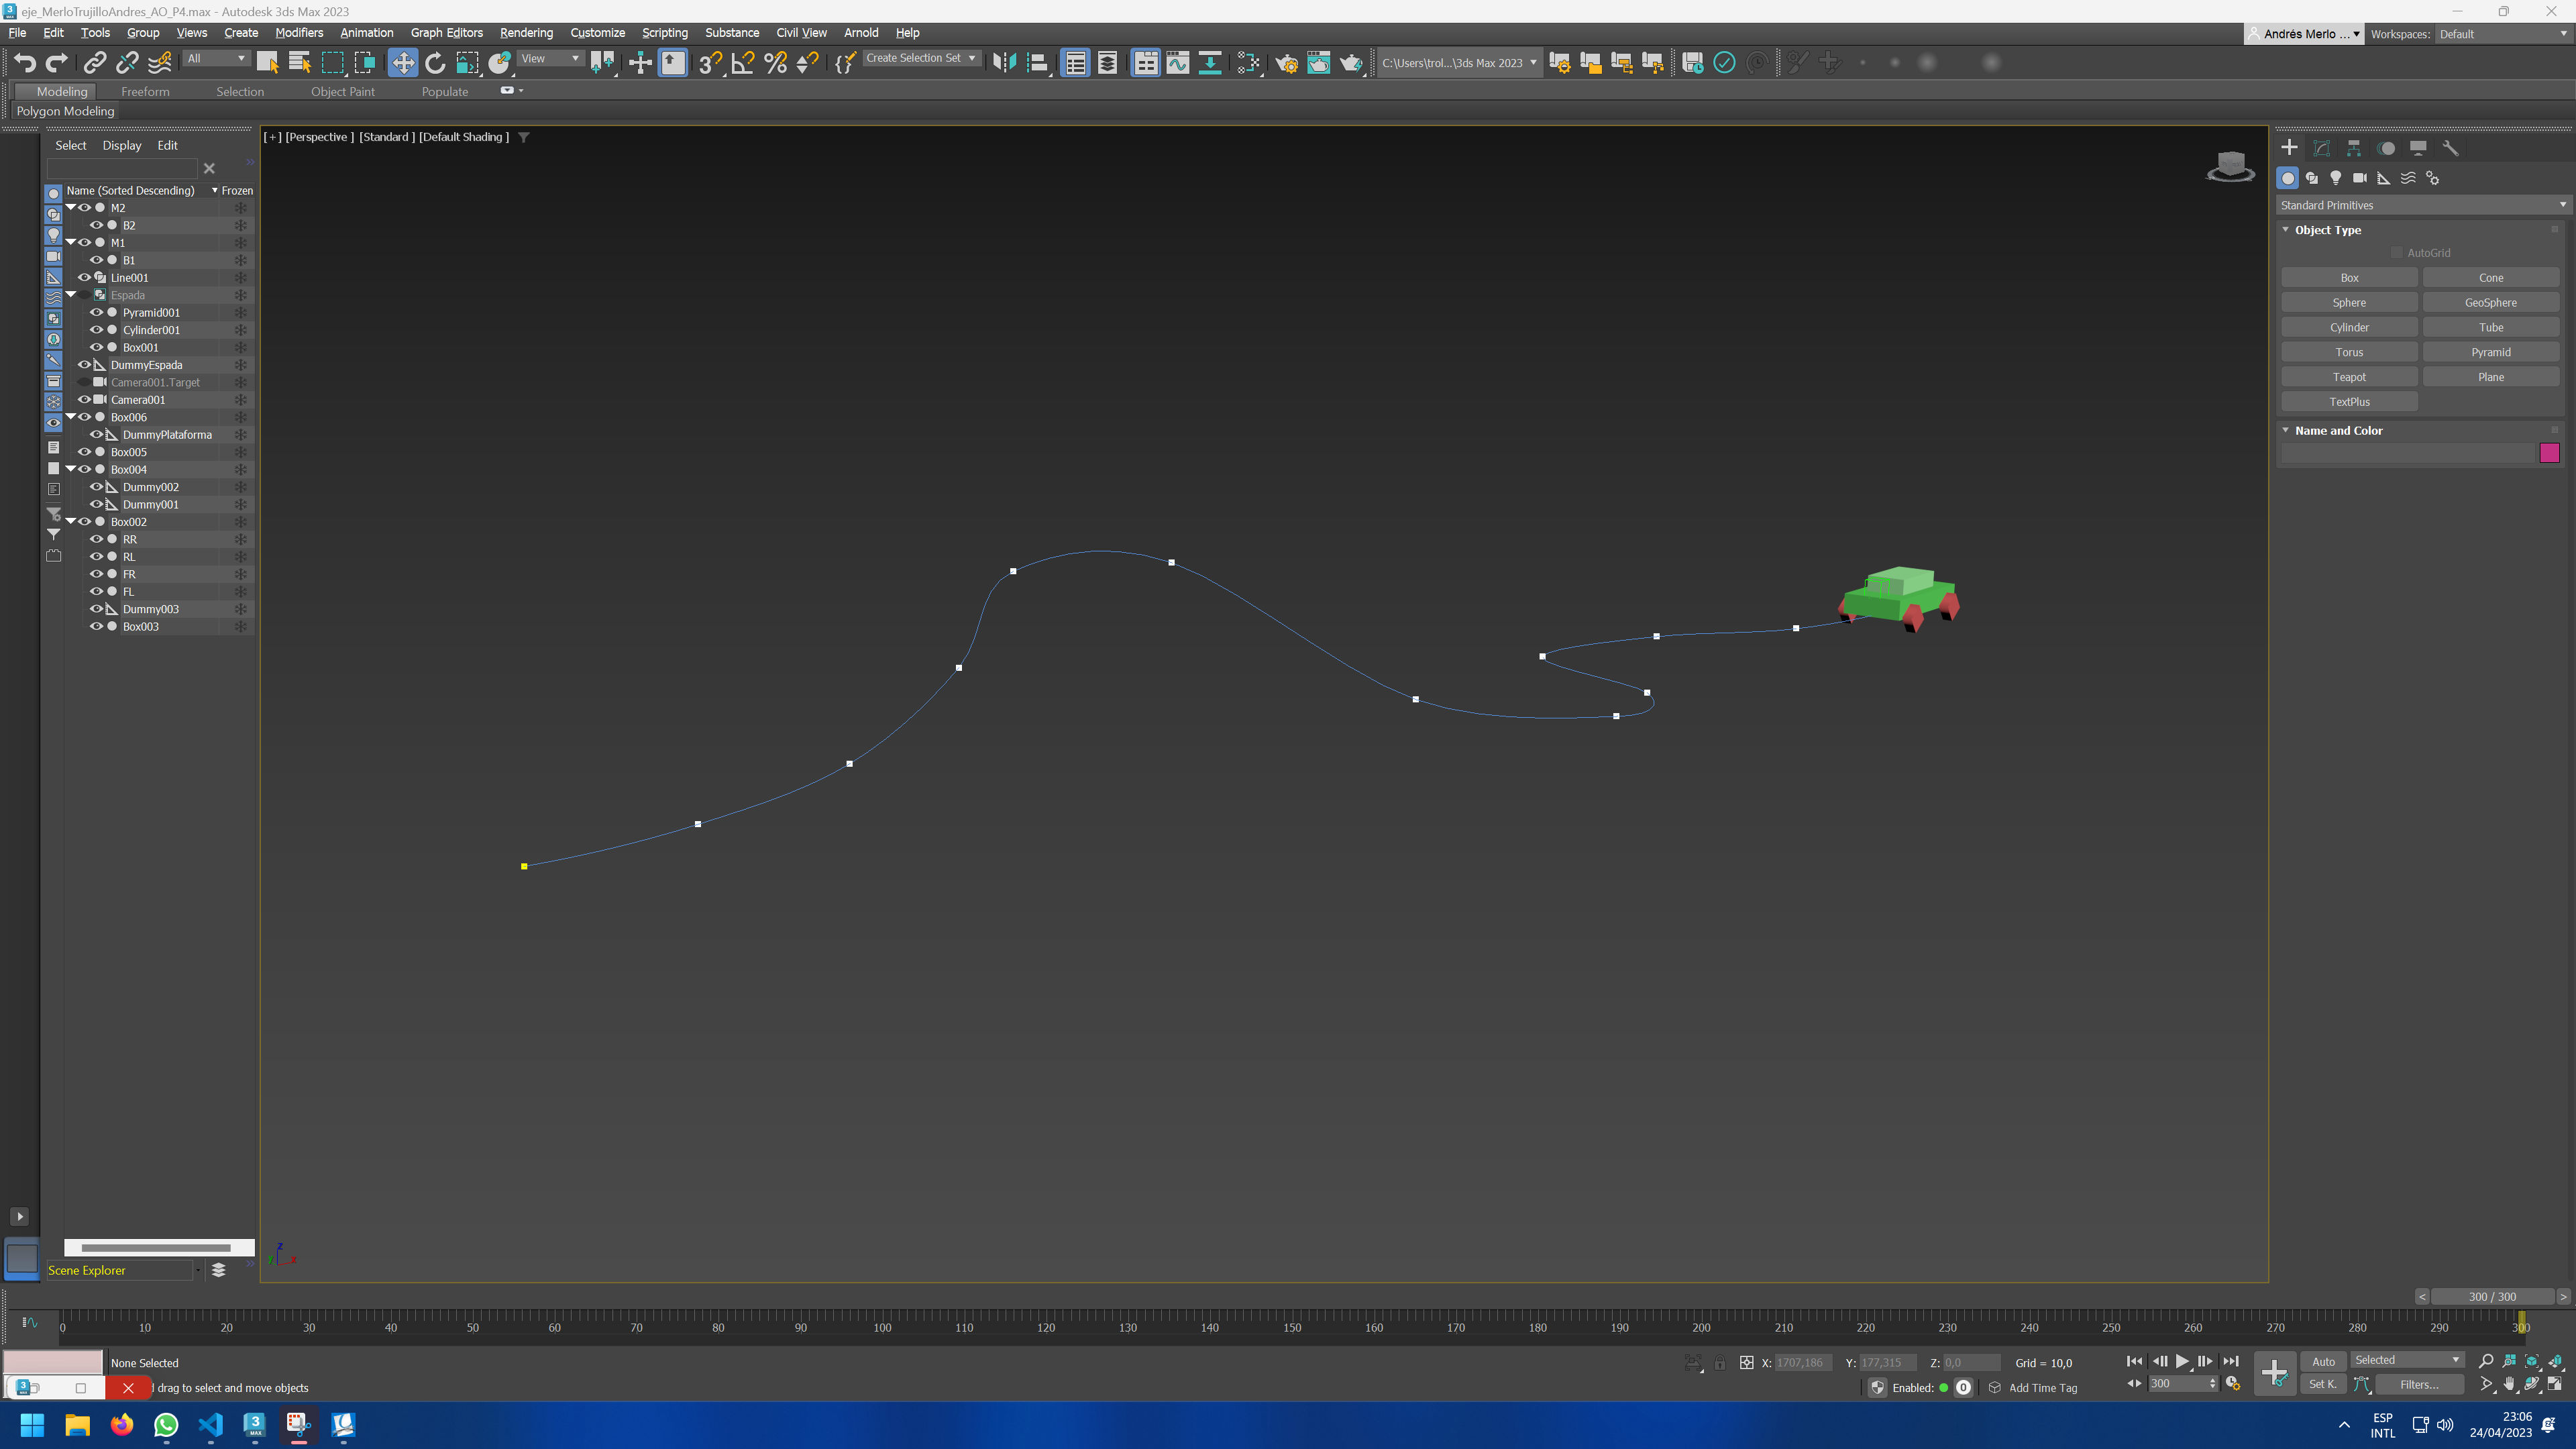
\includegraphics[width=\textwidth]{imagenes/coche/keyframes/300.png}
        \caption{Coche en el instante 300.}
    \end{subfigure}
    \caption{Instantes de la animación del \textit{Path Constraint}.}
\end{figure}

Y a continuación hay algunas capturas para mostrar la rotación de las ruedas:

\begin{figure}[H]
    \centering
    \begin{subfigure}[t]{0.48\textwidth}
        \centering
        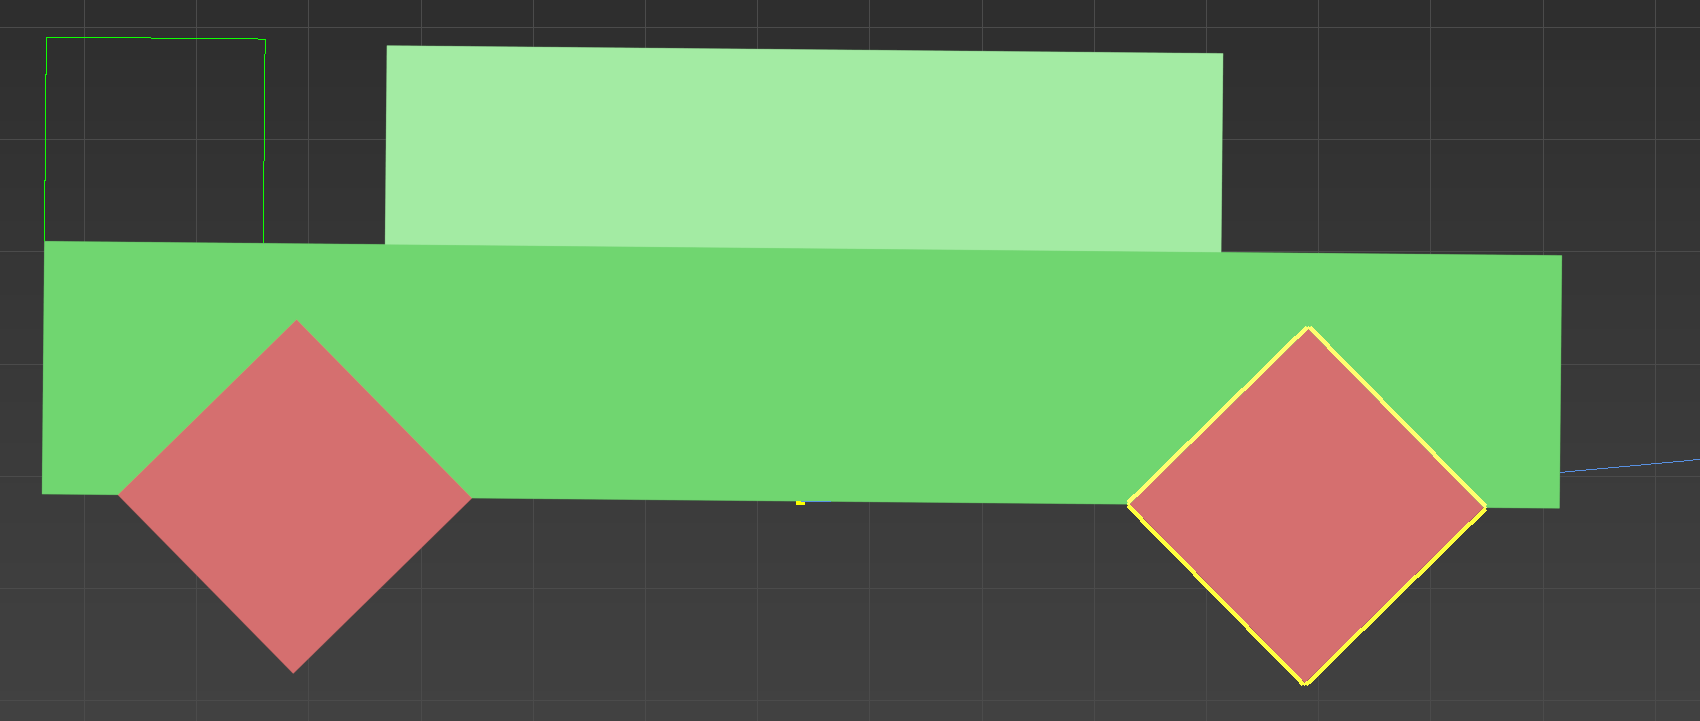
\includegraphics[width=\textwidth]{imagenes/coche/ruedas/antes.png}
        \caption{Ruedas de la derecha en el instante 150.}
    \end{subfigure}
    \hfill
    \begin{subfigure}[t]{0.48\textwidth}
        \centering
        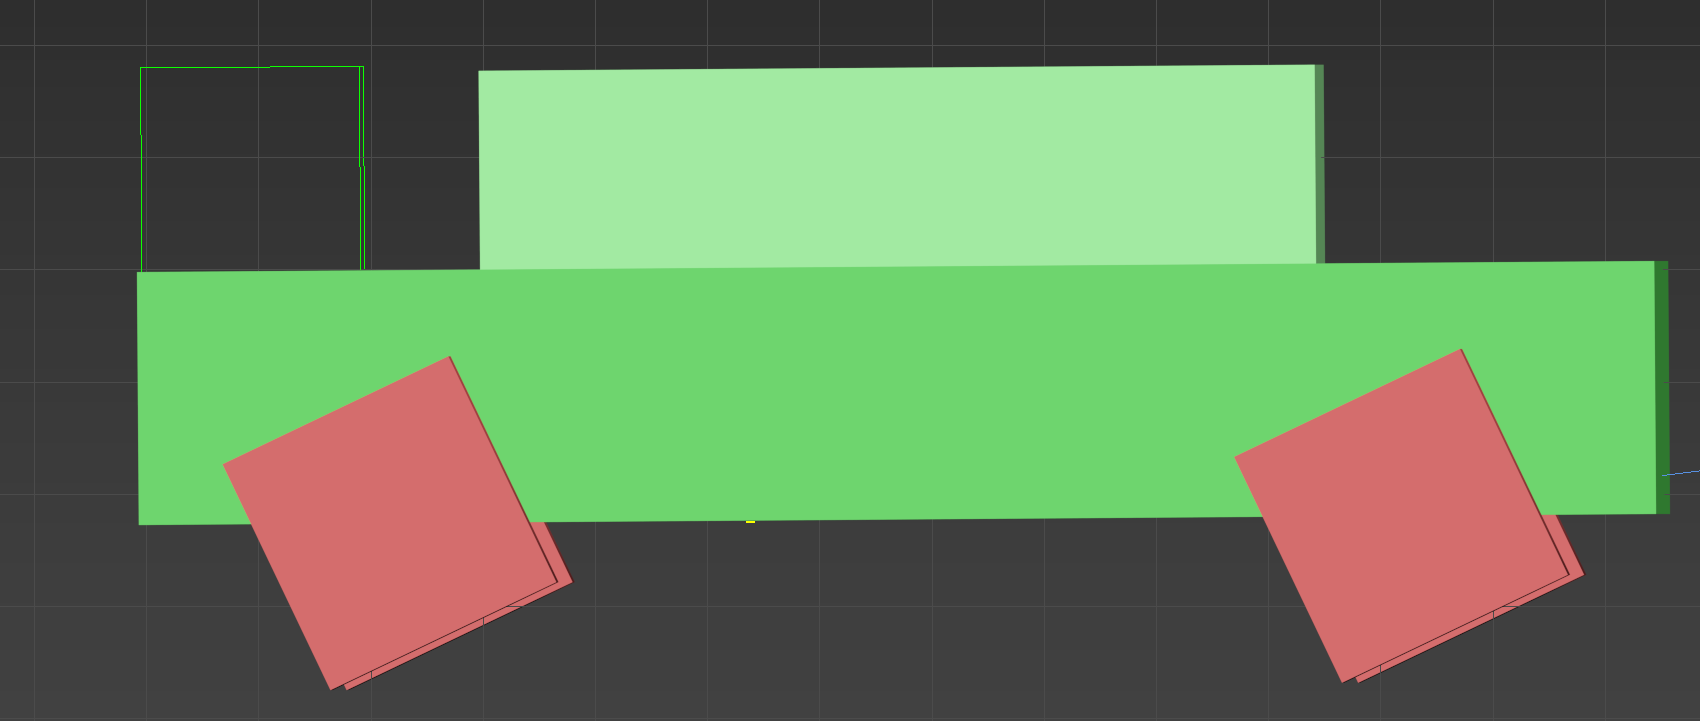
\includegraphics[width=\textwidth]{imagenes/coche/ruedas/despues.png}
        \caption{Rueda de la derecha en el instante 151.}
    \end{subfigure}
    \caption{Movimiento de las ruedas del coche.}
\end{figure}
\section{Cámara}

Para la cámara he utilizado una de tipo \textit{Target}, cuya posición comienza en la izquierda de la escena.

Voy a dividir en dos subsecciones la animación del propio movimiento de la cámara y del seguimiento de los objetos de la escena:

% REVISAR ESTA PARTE PORQUE PUEDE SER QUE HAGA FALTA USAR UN PATH
\subsection{Movimiento de la cámara}

Para realizar el movimiento de pasar de izquierda a la derecha de la escena lo he animado de forma manual usando los siguientes \textit{keyframes}:

\begin{itemize}
    \item \textbf{Instante : }La cámara se encuentra a la izquierda de la escena.
    \item \textbf{Instante : }La cámara se encuentra a la derecha de la escena.
\end{itemize}

\bigskip

Las curvas de animación son las siguientes: 

% curvas de animacion
\begin{figure}[H]
    \centering
   \includegraphics[width=0.5\textwidth]{example-image-a}
\end{figure}
\begin{figure}[H]
    \centering
   \includegraphics[width=0.5\textwidth]{example-image-b}
\end{figure}

% explicacion de las curvas
\blindtext

\subsection{Seguimiento de los objetos}

Para realizar el seguimiento de los objetos he utilizado en el \textit{target} de la cámara una restricción de posición (\textit{Position Constraint}), cuyos objetivos son la espada y el coche.

\bigskip

Estos pesos deben cambiar cuando el coche proceda a moverse, para pasar de fijarse en la espada al propio coche. Los \textit{keyframes} de esta restricción son:

\begin{itemize}
    \item \textbf{Instante : }El \textit{target} está fijado completamente en la espada y la está siguiendo.
    \item \textbf{Instante : }El \textit{target} ahora está fijándose completamente en el coche y lo sigue.
\end{itemize}

\bigskip

En cuanto a las curvas de animación utilizadas, son las siguientes:

\begin{figure}[H]
    \centering
   \includegraphics[width=0.5\textwidth]{example-image-a}
\end{figure}
\begin{figure}[H]
    \centering
   \includegraphics[width=0.5\textwidth]{example-image-b}
\end{figure}

% explicacion
\blindtext
\section{Configuración de la espada}

Ya se ha explicado en otras secciones por separado, pero me gustaría repetirlo todo de nuevo en una sola sección para más claridad.

\bigskip

La espada tiene dos restricciones, que dividiré en subsecciones distintas a continuación:

\subsection{Position Constraint}

Para que la espada se quede pegada a las manos y a la plataforma, es necesario usar el \textit{Position Constraint} cuyos objetivos sean ambas manos y un \textit{dummy} que hay en la plataforma.

\bigskip

Para realizar el cambio de un objeto a otro, es necesario cambiar sus pesos mediante \textit{keyframes}. Por tanto, los instantes más importantes son: 

\begin{itemize}
    \item \textbf{Instante 20: }El peso de la restricción se encuentra en la mano izquierda del todo.
    \item \textbf{Instante 27: }Ahora el peso de la restricción se encuentra del todo en la otra mano.
    \item \textbf{Instante 65: }El peso se sigue manteniendo en la mano derecha.
    \item \textbf{Instante 70: }Ahora el peso se encuentra en el \textit{dummy} de la plataforma.
\end{itemize}

\bigskip

Las curvas de animación son:

\begin{figure}[H]
    \centering
    % curvas
    \begin{subfigure}[t]{0.27\textwidth}
        \centering
        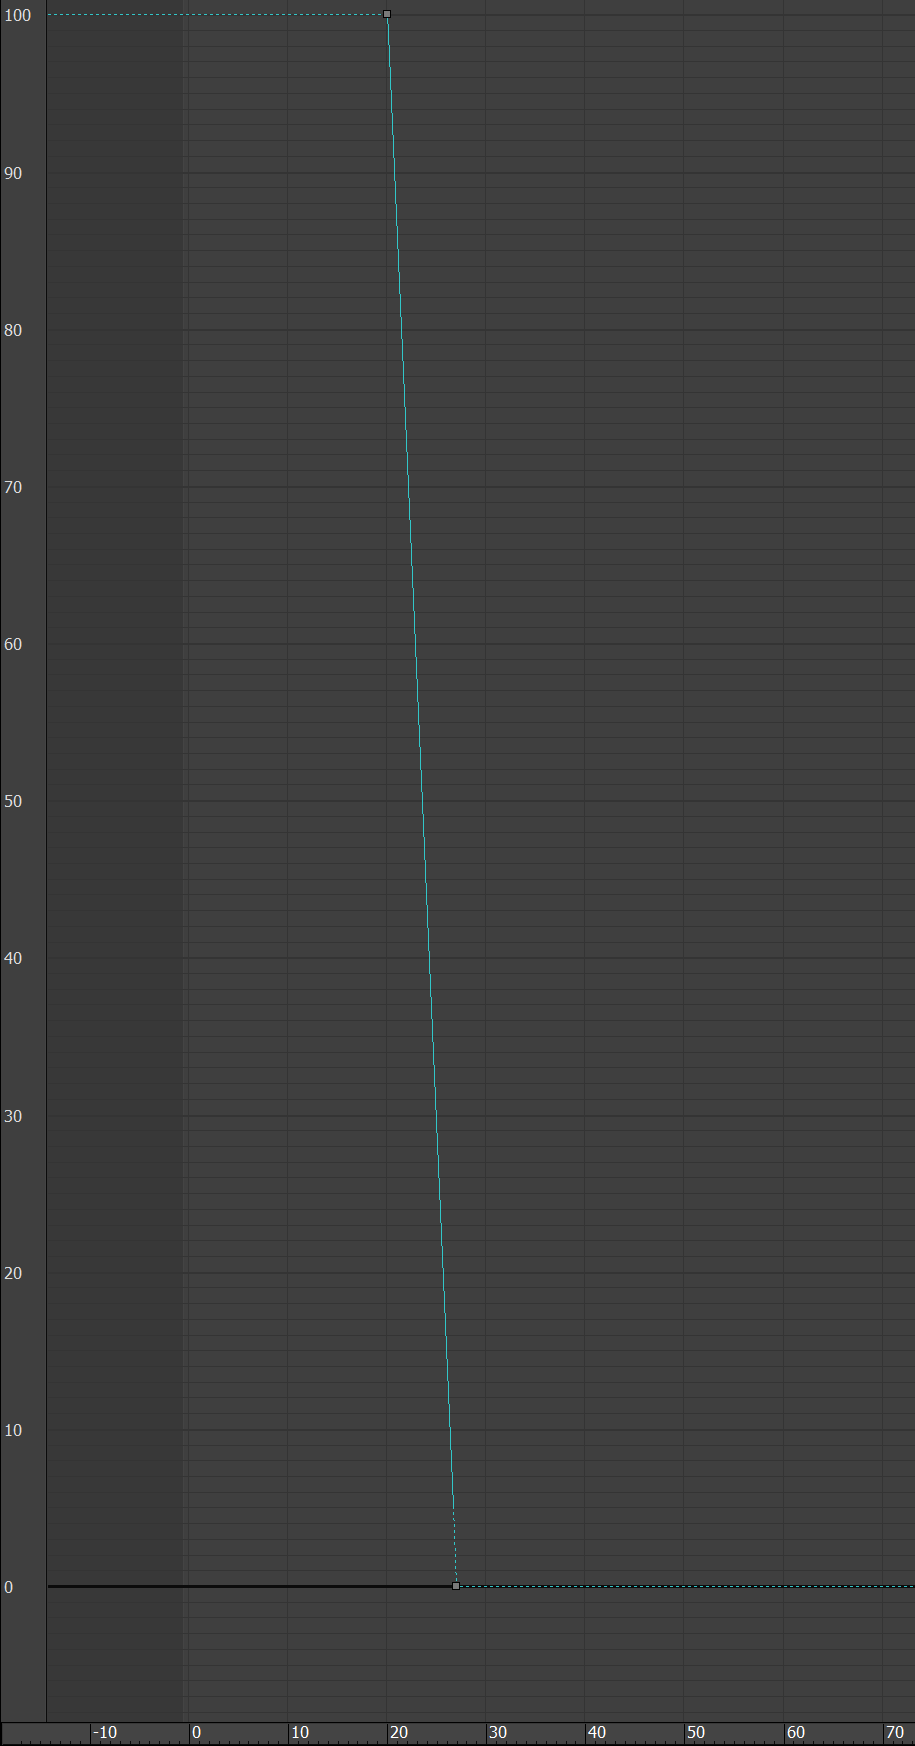
\includegraphics[width=\textwidth]{imagenes/espada/peso0.png}
        \caption{Curva que representa el peso de la mano izquierda con respecto al tiempo.}
     \end{subfigure}
    \hfill
     \begin{subfigure}[t]{0.27\textwidth}
        \centering
        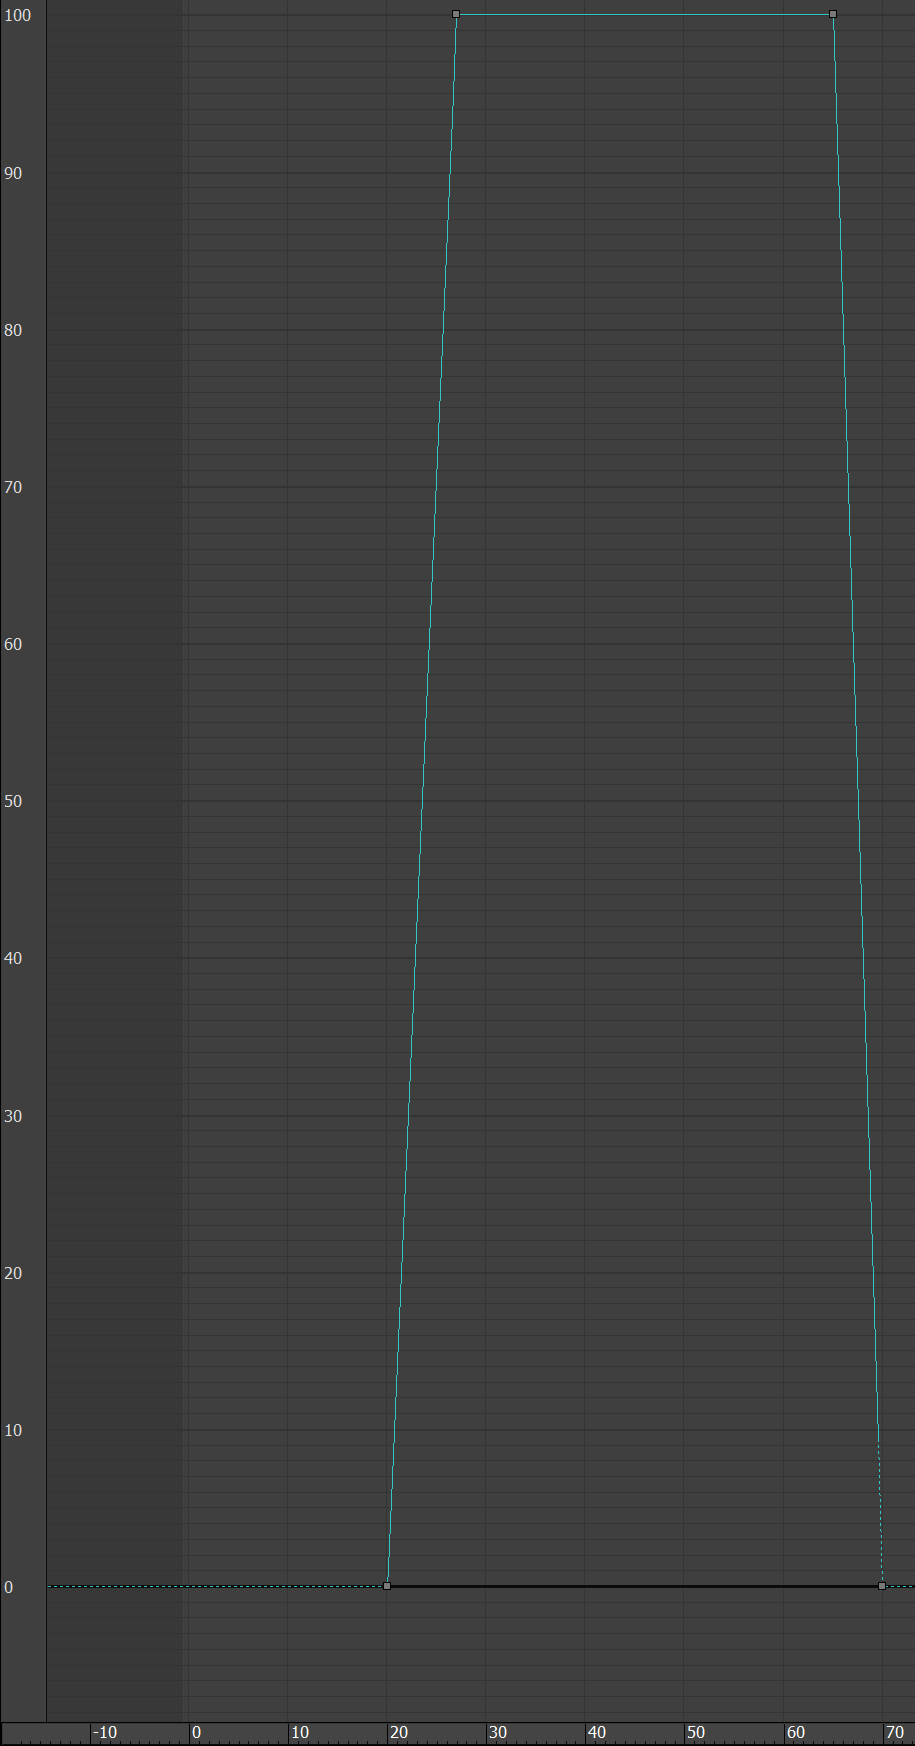
\includegraphics[width=\textwidth]{imagenes/espada/peso1.png}
        \caption{Curva que representa el peso de la mano derecha con respecto al tiempo.}
     \end{subfigure}
    \hfill
     \begin{subfigure}[t]{0.27\textwidth}
        \centering
        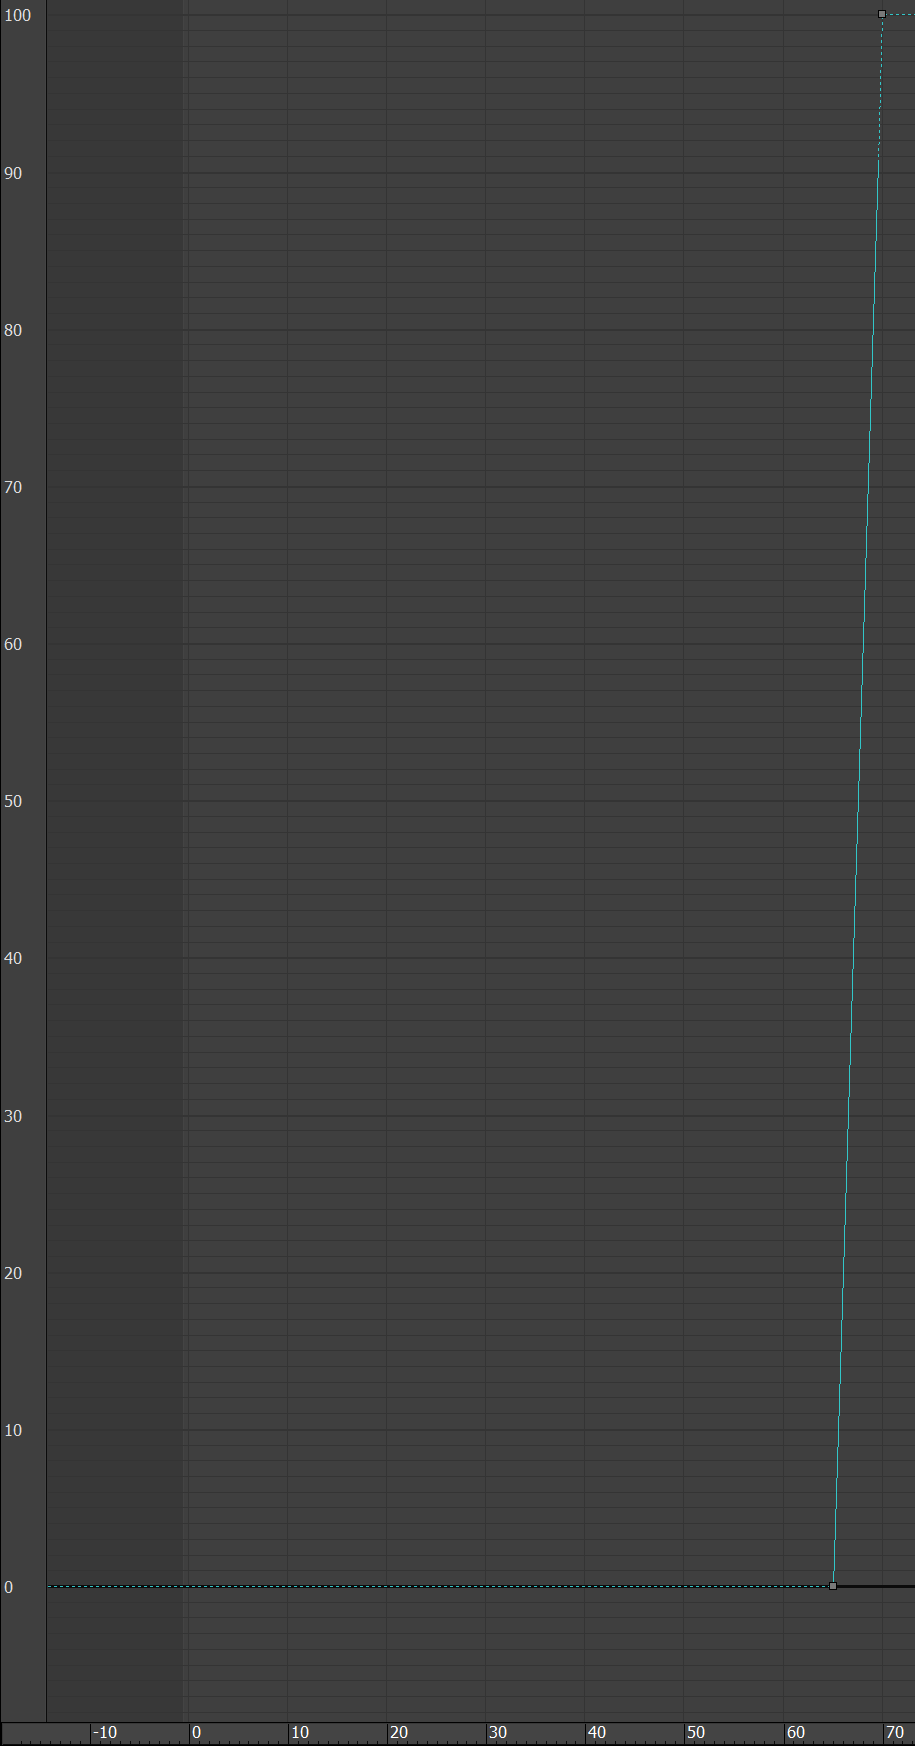
\includegraphics[width=\textwidth]{imagenes/espada/peso2.png}
        \caption{Curva que representa el peso de la plataforma con respecto al tiempo.}
     \end{subfigure}
     \caption{Curvas de los pesos del \textit{Position Constraint}.}
 \end{figure}

Como dije en la sección de las manos, he usado para el cambio de manos una curva de aceleración y al final lineal, para simular el lanzamiento de la espada de una mano a otra. En cuanto al cambio de la plataforma, al no tener animación el cambio de pesos, he decidido hacerlo también para ser consistente.


\bigskip

El resultado final es que la espada pasa de una mano a otra, después la mano de la derecha deja la espada en la plataforma y finalmente la grúa se mueve con la espada encima.


\subsection{LookAt Constraint}

Una vez que la espada ha subido en la plataforma, es necesario hacer que siga el recorrido del coche. Para ello se debe usar un \textit{LookAt Constraint} en el eje Z, que permite fijarse en el objeto que tenga como objetivo. 

\bigskip

No obstante, si solo se elige como objetivo el coche, la espada quedará torcida desde un primer momento, ya que va a estar mirándolo. Una forma de solucionarlo es usando un \textit{Dummy} con una restricción \textit{Link} en las manos y la plataforma, para que siga siempre encima de la espada. Además, he limitado el movimiento de esta restricción a solo la translación en los 3 ejes.

\bigskip

Como dije en el apartado del coche, esto se puede hacer yendo a: \textit{Hierarchy} $\rightarrow$ \textit{Link Info}.

\begin{figure}[H]
    \centering
   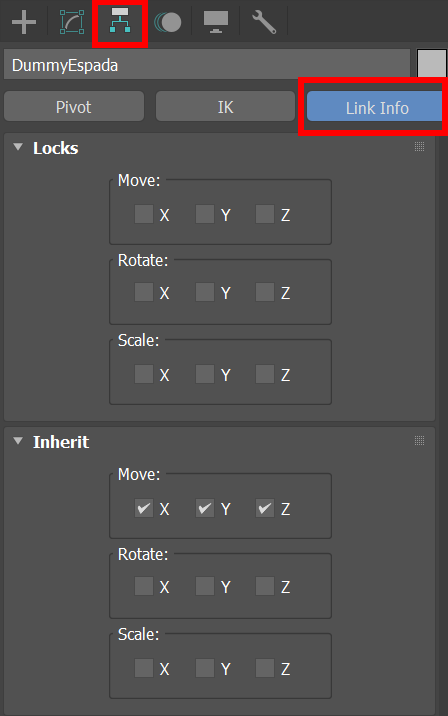
\includegraphics[width=0.35\textwidth]{imagenes/espada/dummyTopHierarchy.png}
   \caption{Menú para bloquear canales.}
\end{figure}

Poniendo como objetivo en el \textit{LookAt Constraint} este \textit{dummy}, ya se ha solucionado el problema, pero hay que cambiar el peso cuando la espada se encuentre arriba para que mire al coche.

\bigskip

Por tanto, los \textit{keyframes} son:

\begin{itemize}
    \item \textbf{Instante 125: }El peso de la restricción está completamente en el \textit{dummy} superior.
    \item \textbf{Instante 150: }El peso de la restricción está completamente en el \textit{dummy} del coche para que lo siga en su trayecto.
\end{itemize}

\bigskip

La curva de animación es las siguientes:

\begin{figure}[H]
    \centering
   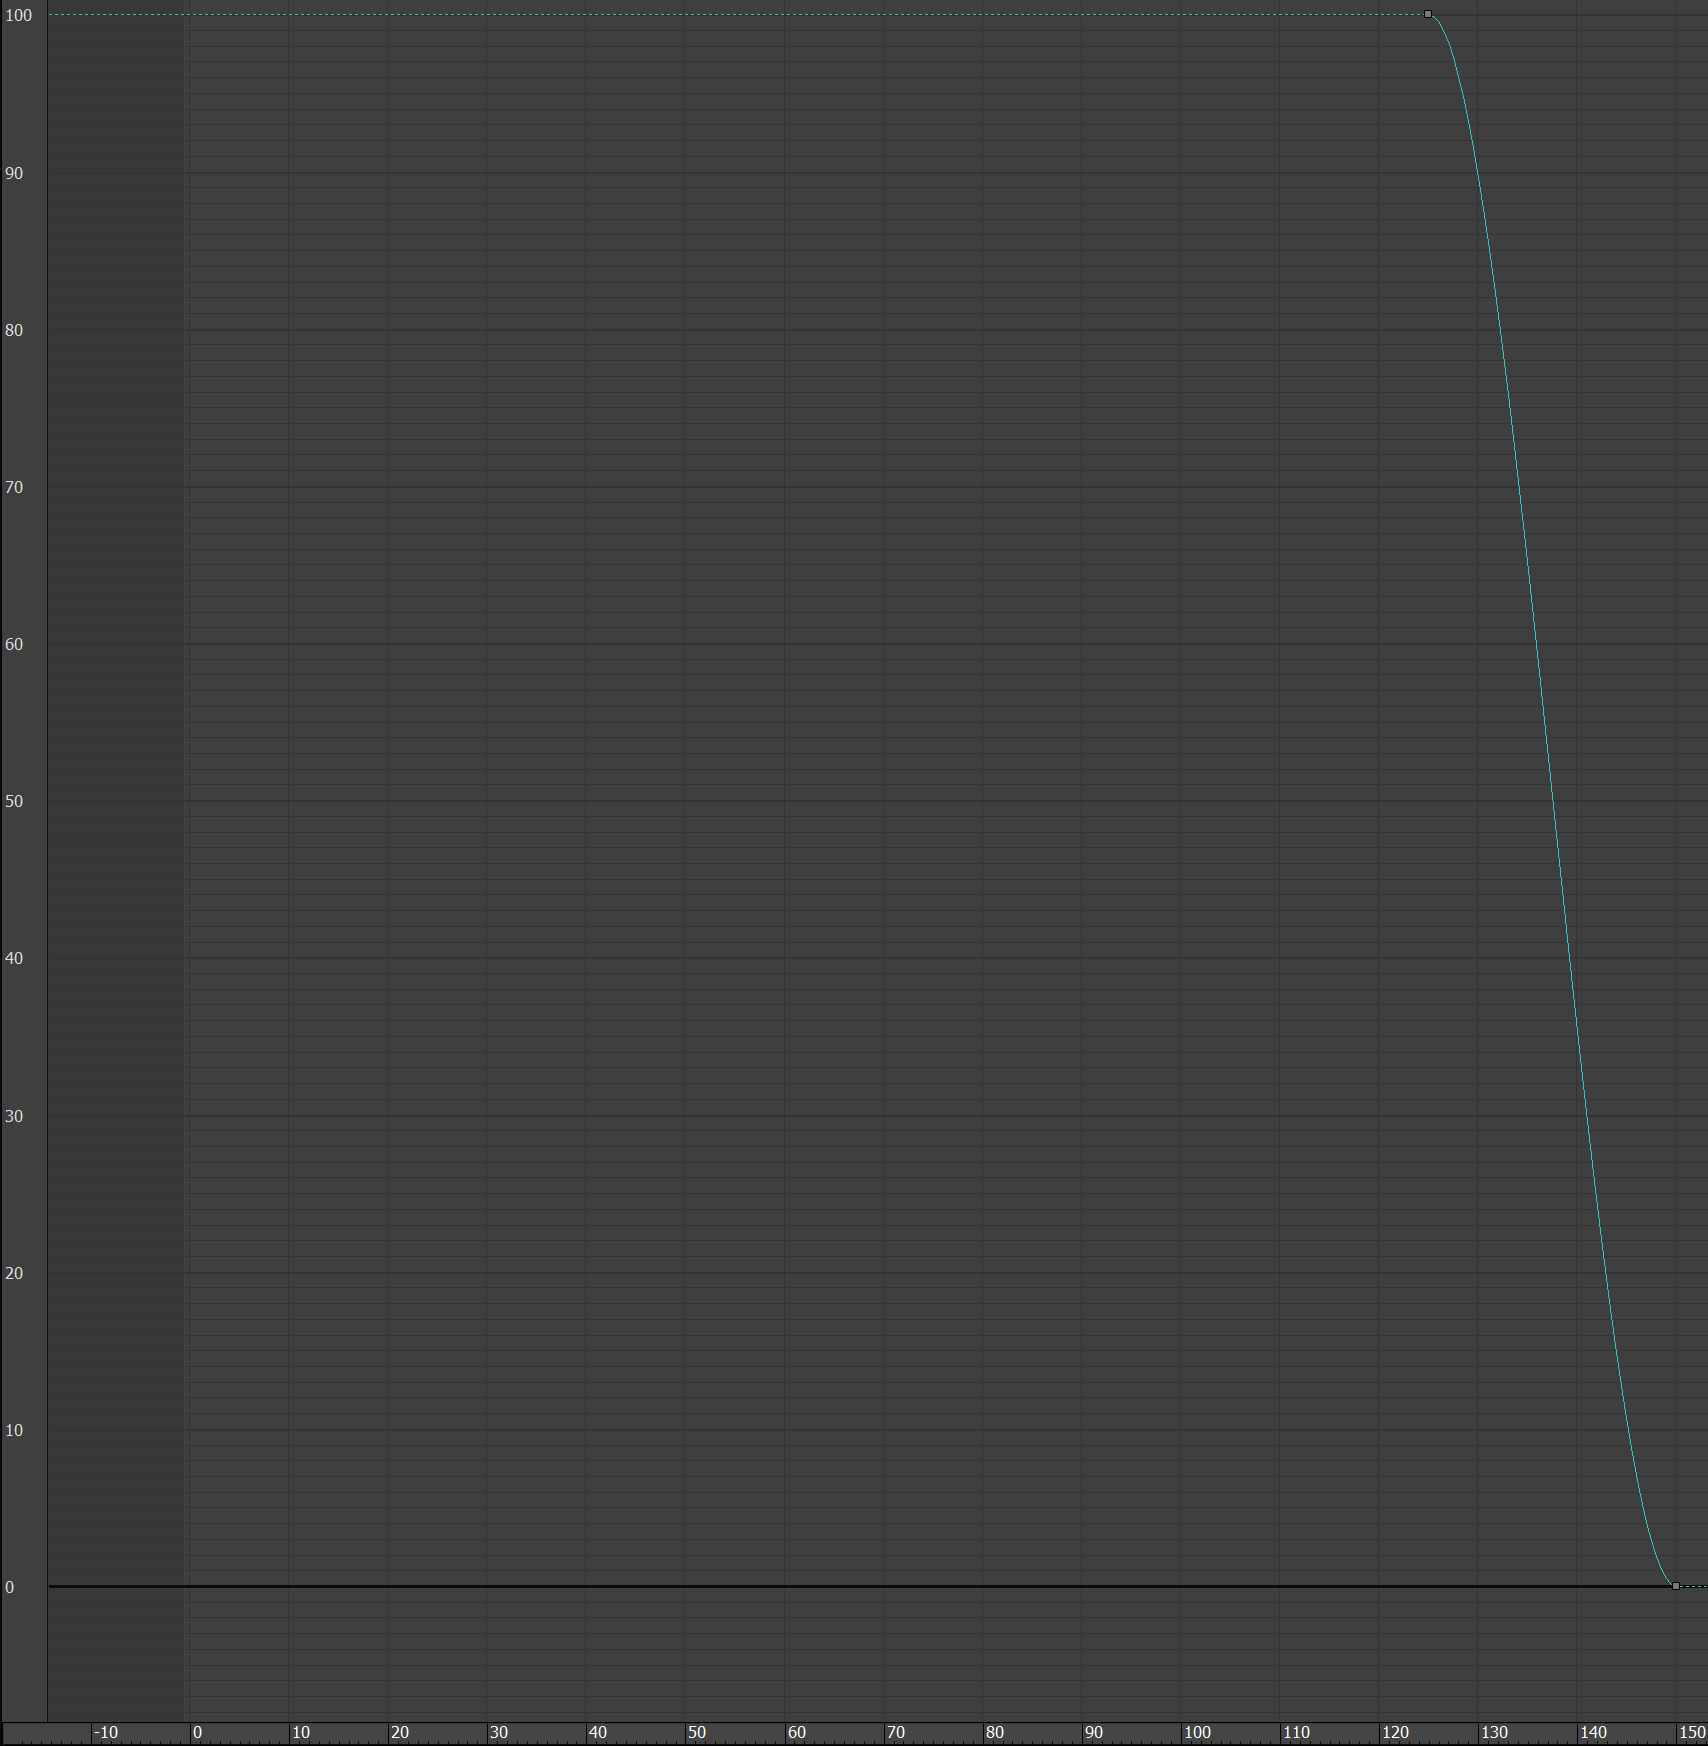
\includegraphics[width=0.6\textwidth]{imagenes/espada/lookat0.png}
   \caption{Curva usada para realizar el cambio de pesos en la restricción en el objetivo del \textit{dummy}.}
\end{figure}

\begin{figure}[H]
    \centering
   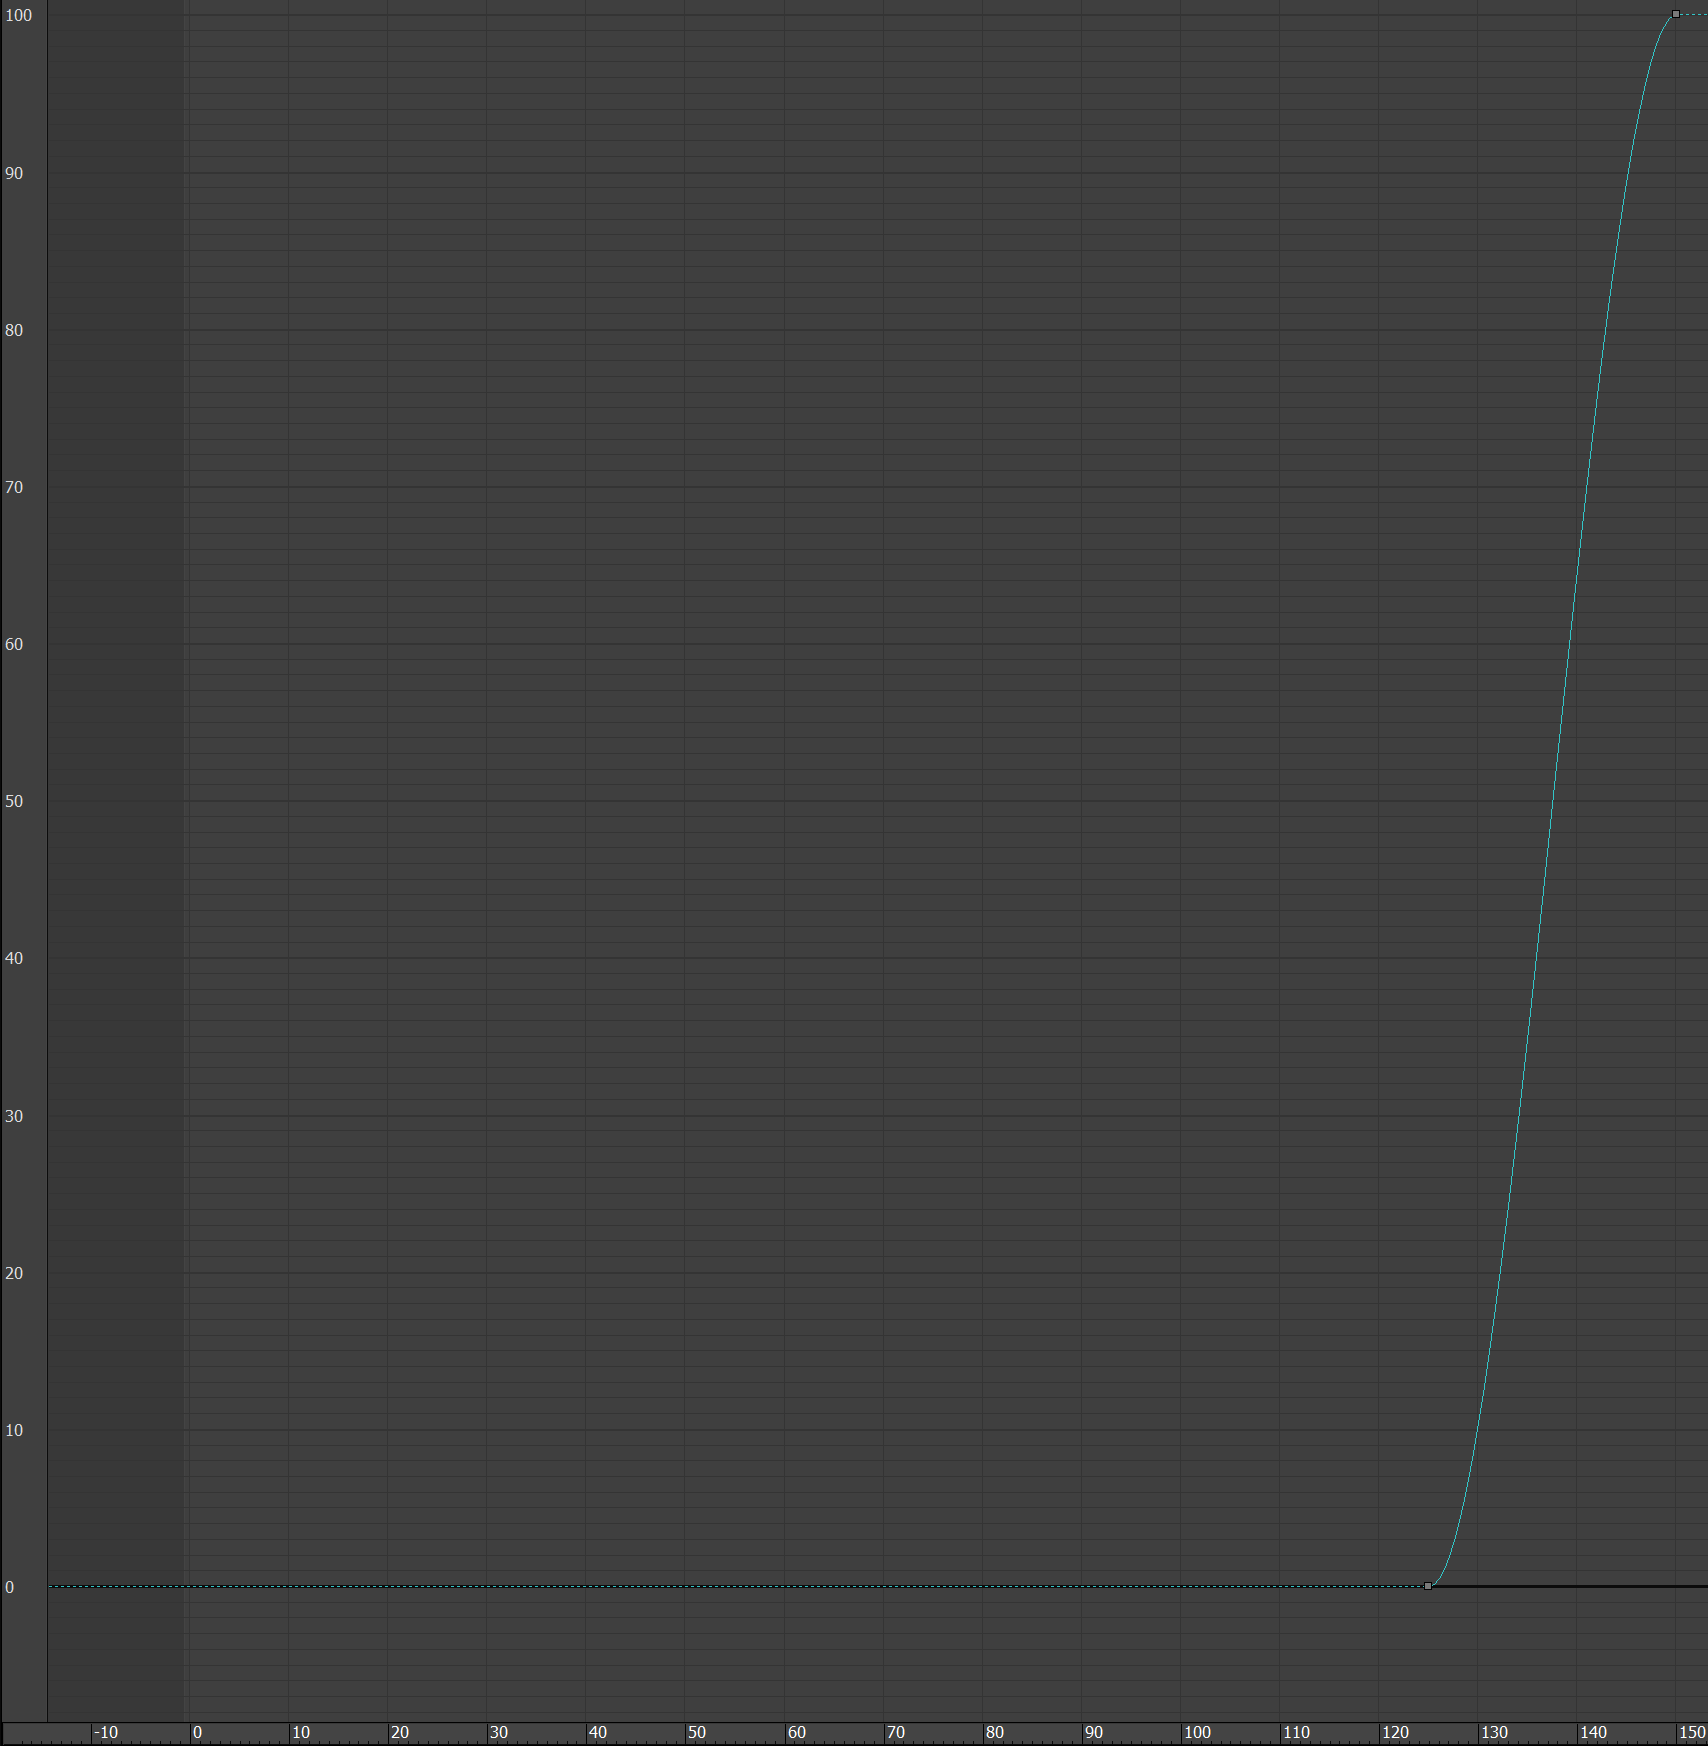
\includegraphics[width=0.6\textwidth]{imagenes/espada/lookat1.png}
   \caption{Curva usada para realizar el cambio de pesos en la restricción en el objetivo del \textit{dummy} del coche.}
\end{figure}

Como se puede observar, he usado la forma por defecto, ya que es la que me ha resultado más suave y realista.

\section{Resultado final}

El resultado final de la animación es el siguiente:

\begin{figure}[H]
    \centering
   \includegraphics[width=0.5\textwidth]{example-image-a}
\end{figure}
\begin{figure}[H]
    \centering
   \includegraphics[width=0.5\textwidth]{example-image-b}
\end{figure}
\begin{figure}[H]
    \centering
   \includegraphics[width=0.5\textwidth]{example-image-c}
\end{figure}

\begin{figure}[H]
    \centering
   \includegraphics[width=0.5\textwidth]{example-image-a}
\end{figure}
\begin{figure}[H]
    \centering
   \includegraphics[width=0.5\textwidth]{example-image-b}
\end{figure}
\begin{figure}[H]
    \centering
   \includegraphics[width=0.5\textwidth]{example-image-c}
\end{figure}

\begin{figure}[H]
    \centering
   \includegraphics[width=0.5\textwidth]{example-image-a}
\end{figure}
\begin{figure}[H]
    \centering
   \includegraphics[width=0.5\textwidth]{example-image-b}
\end{figure}
\begin{figure}[H]
    \centering
   \includegraphics[width=0.5\textwidth]{example-image-c}
\end{figure}

\begin{figure}[H]
    \centering
   \includegraphics[width=0.5\textwidth]{example-image-a}
\end{figure}
\begin{figure}[H]
    \centering
   \includegraphics[width=0.5\textwidth]{example-image-b}
\end{figure}
\begin{figure}[H]
    \centering
   \includegraphics[width=0.5\textwidth]{example-image-c}
\end{figure}

\end{document}
